\documentclass[oneside,a4paper,12pt]{article} % Specifies the page format and font size.



% -------------------------------------- Integration of packages --------------------------------------
% Literature and language
\usepackage[english]{babel}
\usepackage{csquotes}
\usepackage[style=apa6,backend=biber]{biblatex}
\DeclareLanguageMapping{british}{british-apa}
% \renewcommand{\thepage}{} % Removes the page number
\addbibresource{Content/bibliography.bib}
\usepackage{xurl} % url breaks in biblatex
% https://tex.stackexchange.com/questions/567789/adding-line-break-to-bibliography-with-long-numerical-doi

% Format and layout
\usepackage[left=3cm,right=3cm,bottom=3cm]{geometry} % Specifies left and right side margins.
\usepackage{setspace} % Package that enables modifying the line spacing.
\setstretch{1.3} % Sets a line spacing of 1.3.
\parindent0pt % Sets the left indent at a new paragraph.
 \parskip10pt % Sets the space between two paragraphs.
\usepackage{footmisc} % Implements a range of footnote options.
\renewcommand{\footnotelayout}{\setstretch{1}} % Sets a line spacing of 1 for the footnotes.
\pagestyle{headings} % Creates a header using the page number and the heading of the current section.
\usepackage{eurosym} % Usage of €
\usepackage[all]{nowidow} % avoid widows https://tex.stackexchange.com/a/30409/169093
\usepackage{pdflscape}

% Colors
\usepackage{xcolor} % Enables the definition of more colors.

\definecolor{viz-green}{RGB}{0,150,0}
\definecolor{viz-red}{RGB}{150,0,0}
\definecolor{viz-red}{HTML}{FF0000}
\definecolor{viz-gray}{HTML}{D6DCE5}
\definecolor{viz-white}{HTML}{FFFFFF}
\usepackage{colorprofiles} % load color profiles for pdf/a standard

% https://tex.stackexchange.com/questions/188533/how-to-draw-squares-circles-and-triangles
\usepackage{tikz}
\usetikzlibrary{shapes}

\newcommand{\mysquare}[1]{\tikz{\node[draw=#1,fill=#1,rectangle,minimum
width=0.2cm,minimum height=0.2cm,inner sep=0pt] at (0,0) {};}}

\newcommand{\mycircle}[1]{\tikz{\node[draw=black,fill=#1,circle,minimum
width=0.2cm,minimum height=0.2cm,inner sep=0pt] at (0,0) {};}}

\newcommand{\mytriangle}[1]{\tikz{\node[draw=#1,fill=#1,isosceles
triangle,isosceles triangle stretches,shape border rotate=90,minimum
width=0.2cm,minimum height=0.2cm,inner sep=0pt] at (0,0) {};}}

\newcommand{\bestcircle}{\tikz{\node[circle,draw=darkgray, fill=white, line width=0.5pt, minimum width=0.2cm,minimum height=0.2cm, inner sep=0pt, draw opacity=.2] at (0,0){};}}
\newcommand{\myline}{\tikz{\draw[dashed, gray, line width=1pt] (0,0) -- (0,0.3);}}

\usepackage{enumitem} % enumerate with letters https://tex.stackexchange.com/a/129960

% Tables and Graphs
\usepackage{makecell} %Connected rows
\usepackage{booktabs} % Improves the design of the tables
\usepackage{longtable} % Allows tables to be longer than one page.
\usepackage{threeparttable} % footnotes in tables
\usepackage{threeparttablex} % threeparts table + longtable
\usepackage{multirow,multicol} % With this package it is now possible to combine columns and rows within tables.
\usepackage{graphicx} % Allows to implement graphics.
% \usepackage[font={sf, small}]{subfig} % Enables graphs consisting of several figures.
\usepackage{alphalph}
\usepackage[font={small}]{subfig}
\renewcommand\thesubfigure{\alphalph{\value{subfigure}}}
% \usepackage[font={sf, small}]{floatrow} % enables to format tables
\usepackage[font={small}]{floatrow}

\graphicspath{{./Graphs/}} % Tells LATEX that the images are kept in a folder named images under the directory of the main document.
\usepackage[hypcap=false,font={small}]{caption} % Provides many ways to customize captions.
%\usepackage[hypcap=false,font={sf, small}]{caption} % Provides many ways to customize captions.

\usepackage{siunitx} % Enables the use of SI units e. g., proper handling of percentage

% manually define opening bracket which is otherwise parsed by sunitx
% https://tex.stackexchange.com/q/450026/169093
\usepackage{etoolbox} 
\newrobustcmd{\parl}{(}
\newrobustcmd{\parr}{)}

\newcommand*{\tabindent}{ \hspace{2mm}} % Indentation for tables

\newcommand{\todo}[1]{\textcolor{red}{TODO: #1}\PackageWarning{TODO:}{#1!}} % Todos

\sisetup{round-mode=places,round-precision=2, group-separator={,},output-decimal-marker={.}, round-pad = false, input-symbols = {(-)}, % separate-uncertainty=false,
group-minimum-digits=4, % 1,000 instead of 1000
% table-space-text-pre={(},
% table-align-text-pre=false,
% table-space-text-post={$^{***}$},
table-align-text-post=false,
detect-weight=true,
detect-inline-weight=math,
retain-explicit-plus=true,
% round-integer-to-decimal=false,
round-precision=2,
table-format = 1.3, 
output-exponent-marker=\ensuremath{\mathrm{e}}
} % round to 2 decimal places

\usepackage[super]{nth} % 1st, 2nd etc.
\usepackage{import} % path for inkscape graphics
% Mathematics
 \usepackage{amscd,amsfonts,amsmath,amssymb,amsthm,amscd,bbm} % Extends the math set.

% PDF/a standard
\usepackage[a-2b,mathxmp]{pdfx}

% Depth
\setcounter{secnumdepth}{3}


% prevent footnotes from being split
% https://texfaq.org/FAQ-splitfoot
\interfootnotelinepenalty=10000


% --------------------------------- Information on thesis ---------------------------------
% Please fill in this information once at the beginning. This way, gaps will be filled in automatically in the following.
\newcommand{\name}{Markus Bilz} % Enter your name.
\newcommand{\dateofthesis}{15 July 2023} % Enter the submission date of your thesis.
\newcommand{\titleofthesis}{Improving Option Trade Classification With Machine Learning} % Enter the title of your thesis.
\newcommand{\streetadress}{Mathystr.~14-16 // XI-11} % Enter your street address.
\newcommand{\postalcode}{76133} % Enter your postal code.
\newcommand{\city}{Karlsruhe} % Enter your city/town.
\newcommand{\email}{markus.bilz@student.kit.edu} % Enter your email address.
\newcommand{\typeofthesis}{Master Thesis} % specify the type of thesis: Seminar Thesis, Bachelor Thesis, Master Thesis

%--------------------------------- Information in xmpdata ---------------------------------
% definition from macro doesn't seem to work.
\begin{filecontents*}[overwrite]{\jobname.xmpdata}
\Title{Improving Option Trade Classification With Machine Learning}
\Author{Markus Bilz}
\Language{en-GB}
\Keywords{trade-classification\sep machine-learning\sep transformer \sep gradient-boosting}
\end{filecontents*}

% --------------------------------- Information in description ---------------------------------
\pdfinfo {
 /Title (\titleofthesis)
 /Author (\name)
 /Subject (trade classification using machine learning)
 /Keywords (trade-classification machine-learning transformer gradient-boosting) 
}

% --------------------------------- Definition of hyperlinks ---------------------------------
% Hyperreferences
\usepackage{hyperref}
\urlstyle{tt} % typewriter font for urls
\definecolor{darkblue}{rgb}{0,0,.5}
\hypersetup{
 pdfstartview={FitH},
colorlinks=true,
linkcolor=black,
citecolor=darkblue,
urlcolor=black,
bookmarksopen
}

\usepackage[capitalise, noabbrev]{cleveref} % Enables the use of \cref{} to refer to figures, etc. with Fig.
\creflabelformat{equation}{#2#1#3} % omit round brackets
% https://tex.stackexchange.com/a/121055/169093
\Crefname{appsec}{appendix}{appendices}


\usepackage[symbols,acronyms,automake,savewrites=true,toc,section=section,nogroupskip=false,nopostdot]{glossaries}

\setlength{\glslistdottedwidth}{.2\linewidth}

\glsaddkey
 {unit}
 {}
 {\glsentryunit}
 {\Glsentryunit}
 {\glsunit}
 {\Glsunit}
 {\GLSunit}

\makeglossaries

% https://tex.stackexchange.com/questions/98494/glossaries-dont-print-single-occurences/230664#230664
\glsenableentrycount % if only used once, dont abbreviate

\newacronym{ADR}{ADR}{American depository receipt}
\newacronym{ANN}{ANN}{artificial neural network}
\newacronym{ATM}{ATM}{at-the-money}
\newacronym{AUC}{AUC}{area under the curve}
\newacronym{BERT}{BERT}{Bidirectional Encoder Representations from Transformers}
\newacronym{BVC}{BVC}{bulk volume classification}
\newacronym{CRSP}{CRSP}{Center for Research in Securities Prices}
\newacronym{CBOE}{CBOE}{Chicago Board Options Exchange}
\newacronym{CLNV}{CLNV}{Chakrabarty-Li-Nguyen-Van-Ness}
\newacronym{EMO}{EMO}{Ellis-Michaely-O’Hara}
\newacronym{ETF}{ETF}{exchange-traded fund}
\newacronym{FFN}{FFN}{feed-forward network}
\newacronym{FS}{FS}{feature set}
\newacronym{ISE}{ISE}{International Securities Exchange}
\newacronym{ITM}{ITM}{in-the-money}
\newacronym{GBRT}{GBRT}{gradient-boosted regression tree}
\newacronym{GPU}{GPU}{graphics processing unit}
\newacronym{GSU}{GSU}{Grauer-Schuster-Uhrig-Homburg}
\newacronym{LIME}{LIME}{Local Interpretable Model-agnostic Explanations}
\newacronym{LR}{LR}{Lee-Ready}
\newacronym{MCC}{MCC}{Matthews correlation coefficient}
\newacronym{ML}{ML}{machine learning}
\newacronym{MLP}{MLP}{multi-layer perceptron}
\newacronym{MLM}{MLM}{masked language modeling}
\newacronym[first={national best bid and offer}]{NBBO}{NBBO}{national best bid and offer}
\newacronym{NYSE}{NYSE}{New York Stock Exchange}
\newacronym{NASDAQ}{NASDAQ}{National Association of Securities Dealers Automated Quotations}
\newacronym{OTM}{OTM}{out-of-the-money}
\newacronym{RMSE}{RMSE}{root mean squared error}
\newacronym{RF}{RF}{random forest}
\newacronym{ReLU}{ReLU}{Rectified Linear Unit}
\newacronym{SAGE}{SAGE}{Shapley Additive Global importancE}
\newacronym{SSE}{SSE}{sum of squared errors}
\newacronym{SHAP}{SHAP}{SHapley Additive exPlanations}
\newacronym{TRACE}{TRACE}{Trade Reporting and Compliance Engine}
\newacronym{RTD}{RTD}{random token replacement}


%Glossary
\newglossaryentry{activation-function}{name={activation function},plural={activation functions}, description={An activation function is a function, that breaks up the linearity of the neural network. It determines if neurons are activated or not. Common variants include \gls{ReLU} and Softmax.}}
\newglossaryentry{embedding}{name={embedding},plural={embeddings},description={Numerical vector representation of the input, e.g., a word, category, or scalar.}}
\newglossaryentry{feed-forward-network}{name={feed-forward network},plural={feed-forward networks},description={Neural networks without recursion. Well-known variants are \glspl{MLP}.}}
\newglossaryentry{overfitting}{name={overfitting},plural={overfitting},description={Creating a model that fits the training data closely, but does not generalize on unseen data.}}
\newglossaryentry{token}{name={token},plural={tokens},description={Item in a vocabulary. For textual data, tokens can be an individual character, sub-word, a word. 
For tabular data, a token corresponds to a column in the data set.}}
\newglossaryentry{exploding-gradient}{name={exploding gradient},plural={exploding gradients},description={Exploding gradients is a problem encountered during training of deep neural networks with backpropagation. Error gradients can accumulate and result in large parameter updates and unstable training of the network. The opposite is the vanishing gradient problem, whereby gradients become successively smaller during backpropagation, resulting in no or small parameter updates. In both cases, the network does not converge.}}

% compile only locally
% \includeonly{Content/Appendix}

% ----------------------------------- Start of document -----------------------------------
\begin{document}
\setcounter{page}{2} % Cover pages and title page are not numbered. Start numbering from page 2.

% Title page
\newgeometry{left=3cm, right=3cm, bottom=2cm}
\begin{titlepage}
		\begin{center}
			{\Large Karlsruhe Institute of Technology \\
			\vspace{0.6cm}
			Institute for Finance\\
			Department of Financial Engineering and Derivatives\\
			Prof. Dr. Marliese Uhrig-Homburg} \\[4.5cm]
			{\large{\typeofthesis}} \\[1.7cm]
			\setstretch{10.0}
			{\Huge {\titleofthesis}}
			\setstretch{1.3} \\[7cm]
		\end{center}
				
		\begin{tabular}{ll}
        Author:     & {\name}\\
                    & {\streetadress}\\
                    & {\postalcode} {\city}\\
					& E-Mail: {\email}\\\\
        Karlsruhe, & {\dateofthesis}\\
    	\end{tabular}
\end{titlepage}
\restoregeometry % Exclude title page (with %) that is not being used.

% Table of contents
\setcounter{page}{1}\renewcommand{\thepage}{\roman{page}} % Sets the numbering to roman small.
\newpage
\tableofcontents

% List of Figures (comment out if there are no figures in the thesis)
\newpage
\listoffigures % Inserts the list of figures.
\addcontentsline{toc}{section}{List of Figures} % Adds the list of figures to the table of contents.

% List of tables (comment out if there are no tables in the thesis)
\newpage
\listoftables % Inserts the list of figures.
\addcontentsline{toc}{section}{List of Tables} % Adds the list of tables to the table of contents.

% \newpage
% \printglossary[title={List of Symbols},type=symbols,style=dotglos]

\newpage
\printglossary[type=\acronymtype, title=List of Abbreviations, style=listdotted]
% \addcontentsline{toc}{section}{List of Abbreviations}

% Main text section
\newpage
\setcounter{page}{1}\renewcommand{\thepage}{\arabic{page}} % Sets the numbering to Arabic.

\section{Introduction}\label{sec:introduction}

Every option trade has a buyer and seller side. For a plethora of problems in option research, it’s also crucial to determine the party that initiated the transaction. Common applications include the study of option demand \autocite[][3]{garleanuDemandBasedOptionPricing2009}, of informational content in option trading \autocites[][631]{huDoesOptionTrading2014}[][882]{panInformationOptionVolume2006}[][1079]{caoInformationalContentOption2005}, of order flow \autocite[][684]{muravyevOrderFlowExpected2016}, or trading costs \autocite[][4980]{muravyevOptionsTradingCosts2020}. 

Despite the clear importance for empirical research, the true initiator of the trade is frequently missing in option data sets and must be inferred using trade classification rules \autocite[][453]{easleyOptionVolumeStock1998}. In consequence, the correctness of empirical studies hinges on the algorithm's ability to accurately identify the trade initiator.

Among the most prevailing variants to sign trades are the tick test \autocite[][240]{hasbrouckTradesQuotesInventories1988}, quote rule \autocite[][41]{harrisDayEndTransactionPrice1989}, and hybrids thereof such as the \gls{LR} algorithm \autocite[][745]{leeInferringTradeDirection1991}, the \gls{EMO} algorithm \autocite[][536]{ellisAccuracyTradeClassification2000}, and the \gls{CLNV} method \autocite[][3809]{chakrabartyTradeClassificationAlgorithms2007}, that infer the trade initiator from adjacent prices and quotes. These heuristics have initially been proposed and tested in the stock market.

For option markets, the works of \textcites[][10--13]{grauerOptionTradeClassification2022}[][887]{savickasInferringDirectionOption2003} raise concerns about the transferability of standard trade signing rules due to deteriorating classification accuracies and systematic misclassifications. The latter is unsettling, as non-random misclassifications ultimately bias the dependent research \autocite[][260]{odders-whiteOccurrenceConsequencesInaccurate2000}.

Recent work of \textcite[][13--16]{grauerOptionTradeClassification2022} partly alleviates the concern by proposing explicit overrides for trade types and by combining multiple heuristics into deep-stacked hybrids, thereby advancing the state-of-the-art performance in option trade classification. By this means, their approach enforces a more sophisticated decision boundary eventually leading to a more accurate classification. Beyond heuristics, however, it remains open, if classifiers \emph{learned} on trade data can improve upon \emph{static} classification rules in terms of performance and robustness.

Our work fills this gap by focusing on machine learning methods to infer the trade initiator in the option market.\footnote{The authors acknowledge support by the federal state of Baden-Württemberg through \href{https://www.bwhpc.de/}{bwHPC}.} Approaching trade classification with machine learning is a logical choice, given its capability to handle high-dimensional trade data and learn complex decision boundaries. This raises the question, \emph{can an alternative machine learning-based classifier improve upon the accuracy of state-of-the-art approaches for option trade classification?}

To answer this question, we model trade classification through Transformers and gradient boosting. We consider the supervised case, where fully-labelled trade data is available, as well as the semi-supervised setting, where trades are partially labelled with the true trade initiator. Our work makes the following contributions:
\begin{enumerate}[label=(\roman*),noitemsep]
    \item We employ state-of-the-art supervised algorithms i.~e., gradient-boosted trees and Transformer networks to the problem of trade classification and benchmark these approaches against rules-based methods. Our approaches outperform all rule-based approaches on \gls{ISE} and \gls{CBOE} data with comparable data requirements. In the application setting, our approaches approximate the true effective spread best.
    \item In a real-world setting, labelled trades are typically scarce, while unlabelled trades are abundant. Motivated by this consideration, we extend the classifiers to learn on both labelled and unlabelled instances through pre-training and self-training procedures. We analyse the effect on classification accuracy and observe that pre-training of Transformers further alleviates accuracy on \gls{ISE} test data.
    \item We strive to identify the most predictive features. Through a game-theoretic approach, our work is the first to consistently attribute the performance of rule-based and machine learning-based classification to individual features. We discover that both paradigms share common features, but machine learning-based classifiers attain higher performance gains and effectively exploit the data. By probing and visualising the attention mechanism in the Transformer, we can strengthen the connection to rule-based classification and reveal that \emph{learned} rules mimic classical rules.
\end{enumerate}

The remainder of this paper is organised as follows. \cref{sec:related-work} reviews publications on trade classification in option markets and using machine learning, thereby underpinning our research framework. \cref{sec:rule-based-approaches} introduces extant methods for rule-based trade classification. \cref{sec:supervised-approaches} discusses and introduces supervised methods for trade classification. Then, \cref{sec:semi-supervised-approaches} extends the previously selected algorithms for the semi-supervised case. We test the models in \cref{sec:empirical-study} in an empirical setting. In \cref{sec:application} we apply our models to the problem of effective spread estimation. Finally, \cref{sec:discussion} discusses and \cref{sec:conclusion} concludes.

\section{Related Work}\label{sec:related-work}

This chapter introduces research on trade classification in option markets and machine learning-based trade classification.

\subsection{Trade Classification in Option Markets}
\label{sec:trade-classification-in-option-markets}

While classical trade classification algorithms are extensively tested in the stock markets (e.g., \textcite[][3806--3821]{chakrabartyTradeClassificationAlgorithms2007}; \textcite[][259--286]{odders-whiteOccurrenceConsequencesInaccurate2000}), few works have examined trade classification in option markets.

\textcite[][883--887]{savickasInferringDirectionOption2003} were the first to compare the tick rule, quote rule, the \gls{LR} algorithm, and the \gls{EMO} rule for options traded at the \gls{CBOE}. The dataset spans a period from 3 July 1995 to 31 December 1995 consisting of \num{869217} matched trades. The authors report the highest accuracies for the quote rule (\SI{78.98}{\percent}) and find that all rules perform worst when applied to index options.\footnote{We formally define accuracy in \cref{sec:evaluation-metric}.} In general, the trade classification rules exhibit significantly lower classification accuracies on options data than with stock data, urging the need for improved classifiers.

The most exhaustive study is the one of \textcite[][1--53]{grauerOptionTradeClassification2022}. The authors test the accuracy of the classical quote rule and tick rule, and hybrids thereof on three large-scale datasets spanning periods from 2005 to 2021. Consistently for options traded at the \gls{CBOE} and \gls{ISE}, classical rules like the popular \gls{LR}  algorithm only achieve accuracies of \SI{62.03}{\percent} or \SI{62.53}{\percent} and are thus significantly smaller than in the stock market. In line with the research of \textcite[][886]{savickasInferringDirectionOption2003}, the reported accuracies are inversely proportional to the rule's reliance on past transaction prices. In particular, the tick rule performs worst with accuracies marginally different from a random guess. Overall, the success rates of classical algorithms deteriorate between both studies and over time. As a remedy, \textcite[][13--15]{grauerOptionTradeClassification2022} introduce two additional rules based on the trade and quote sizes. The depth rule aims to classify midspread trades based on the depth at the bid or ask. Together with the trade size rule, their second rule, which classifies trades with a trade size matching the size of the bid or ask quote, the authors can substantially improve the performance of classical algorithms. Their best ensemble of rules achieves an accuracy between \SI{73}{\percent} and \SI{75}{\percent} surpassing previous approaches by more than \SI{10}{\percent}.

The work of \textcite[][1--53]{grauerOptionTradeClassification2022} is relevant to this thesis for two reasons. First, their analysis, like ours, is based on the same datasets, allowing for a fair comparison between classical rules and machine learning-based predictors.\footnote{We only consider \gls{CBOE} and \gls{ISE} data. The authors additionally evaluate on GEMX data in their latest update dated May 2023, which we cannot consider.} Second, their stacked combinations of the trade size rule, depth rule, and common trade classification algorithms achieve state-of-the-art performance in option trade classification and are thus a rigorous benchmark for our methods.

\subsection{Trade Classification Using Machine Learning}
\label{sec:trade-classification-using-machine-learning}

In the stock market, \textcite[][396--398]{rosenthalModelingTradeDirection2012} bridges the gap between classical trade classification and machine learning by fitting a logistic regression model on lagged and unlagged features innate to the tick rule, quote rule, and \gls{EMO} algorithm, as well as a sector-specific and a time-specific term. Instead of using the rule's discretized outcome as a feature, he models the rules through so-called information strength functions \autocite[][396--398]{rosenthalModelingTradeDirection2012}. The proximity to the quotes, central to the \gls{EMO} algorithm, is thus modeled by a proximity function. Likewise, the information strength of the quote and tick rule is estimated as the log return between the trade price and the midpoint or the previous trade price. However, it only improves the accuracy of the \gls{EMO} algorithm by a marginal \SI{2.00}{\percent} for \gls{NASDAQ} stocks and \SI{1.10}{\percent} for \gls{NYSE} stocks \autocite[][405]{rosenthalModelingTradeDirection2012}. Our work aims to improve the model by exploring non-linear estimators and minimizing data modeling assumptions.

The work of \textcite[][483]{blazejewskiLocalNonParametricModel2005} compares a $k$-nearest neighbor classifier against logistic regression, as well as simple heuristics like the majority vote over past trades for signing trades at the Australian stock exchange. Their results indicate that the parametric $k$-nearest neighbor classifier improves upon a linear logistic regression in terms of classification accuracy, even when trained on fewer features. The work is unique from the remaining works about the feature set definition. Notably, \textcite[][483]{blazejewskiLocalNonParametricModel2005} use no quote or trade prices, but rather the order book volumes, trade sizes, and past trade signs for classification. No accuracies for classical trade signing rules are reported, which impedes a comparison across different works. In line with their results, we focus on non-linear models. Additionally, our paper addresses the mentioned shortcomings by benchmarking against state-of-the-art trade classification rules. We share the idea of using the trade size, as well as the bid and ask sizes for classification for some of our feature sets, but greedily predict using non-historic features.

Closest to our work is a publication by \textcite[][1--58]{ronenMachineLearningTrade2022}. Therein, the authors compare a selection of machine learning algorithms against classical trade signing rules in the bond and stock market. Their comparison is the first to consider logistic regression, a random forest, as well as \glspl{feed-forward-network}. Over a wide range of feature sets the tree-based ensemble consistently outperforms by out-of-sample accuracy the tick rule and \gls{LR} algorithm, as well as all remaining machine learning models. For the TRACE and \gls{NASDAQ} dataset, their best variant of the random forest outperforms the tick rule by \SI{8.30}{\percent} and \SI{3.30}{\percent}, respectively \autocite[][57]{ronenMachineLearningTrade2022}. Whilst the superiority of random forests is consistent for the bond and equity market, fitted classifiers do not transfer across markets, as accuracies diminish in a transfer setting.

The results convincingly demonstrate the potential of machine learning, i.e., of tree-based ensembles, for trade classification. Yet, the comparability of the results is limited by the classifier's reliance on additional features beyond quote and price data. Albeit, \textcite[][13--14]{ronenMachineLearningTrade2022} consider a wide range of approaches, their selection leaves the latest advancements in artificial neural networks and ensemble learning aside and is mainly guided by computational constraints. Even if the focus is on standard techniques, the unclear research agenda concerning model selection, tuning, and testing hampers the transferability of their results to the yet unstudied option market.

In summary, machine learning has been applied successfully in the context of trade classification. A summary is given in \cref{app:literature-ml-tc}. No previous work performs machine learning-based classification in the options markets. Our work fills this gap and models trade classification using machine learning to improve upon extant rules.

\subsection{Research Framework}\label{sec:research-framework}

The selection of machine learning methods in previous works is arbitrary and guided by computational constraints. Additionally, it leaves out advancements in machine learning. To address these limitations, we propose a comprehensive research framework for trade classification, outlined in \cref{fig:research-framework}. 

Our approach revolves around two key ideas. First, we leverage \glspl{GBRT} and Transformers for trade classification. These methods are selected in \cref{sec:supervised-approaches} for their expected performance, scalability, and extensibility and are later enhanced to learn on partially-labeled trades. Second, classical trade classification rules, such as the \gls{LR} algorithm, are realized as a rule-based classifier using a stacking principle described in \cref{sec:stacked-rule}. This allows for a consistent evaluation and model interpretation, eventually bridging the gap between classical trade classification rules and machine learning.

\begin{figure}[!ht]
    \centering
    {\renewcommand\normalsize{\tiny}
        \normalsize
        \input{./Graphs/research-framework.pdf_tex}}
    \caption[Research Framework]{Research framework for trade classification.}
    \label{fig:research-framework}
\end{figure}

To assess the efficiency of our approach, we conduct a comprehensive empirical study. We thoroughly derive the data preparation process and discuss the training setup. All classifiers are then evaluated in terms of accuracy. With the model-agnostic interpretability method \gls{SAGE}, we study the reliance of the models on features and compare feature importances between trade classification rules and our predictors. In turn, attention maps from Transformers yield model-specific insights.

\section{Rule-Based Approaches}\label{sec:rule-based-approaches}

We provide a concise overview of different trade initiator definitions in \cref{sec:trade-initiator} and recall rule-based algorithms for trade classification in \cref{sec:basic-rules}.

\subsection{Trade Initiator}
\label{sec:trade-initiator}

Various definitions for the trade initiator have been proposed in prior
research. Among these, the:

\emph{Chronological view:} \textcite[][267]{odders-whiteOccurrenceConsequencesInaccurate2000} adapts a chronological view based on the order arrival. She defines the initiator of the trade as the party (buyer or seller) who places their order last, chronologically. This definition requires knowledge about the order submission times.

\emph{Immediacy view:} In contrast, \textcite[][94--97]{leeInferringInvestorBehavior2000} equate the trade initiator with the party in demand for immediate execution. Thus, traders placing market orders, immediately executable at whatever price, or executable limit orders, are considered the trade initiator. By contrast, the party placing non-executable limit orders, which may not even result in a trade, is the non-initiator. This definition remains ambiguous for trades resulting from crossed limit orders, matched market orders, or batched orders \autocite[][94--95]{leeInferringInvestorBehavior2000}.
% FIXME: introduce of the notion of demanding/taking away liquidity and providing liquidity

\emph{Positional view:} Independent from the order type and submission time, \textcite[][533]{ellisAccuracyTradeClassification2000} deduce their definition of the trade initiator based on the position of the involved parties opposite to the market maker or broker. The assumption is, that the market maker or broker only provides liquidity to the investor and the trade would not exist without the initial investor's demand.

The appropriate view differs by data availability i.e., if the order type or submission type can be inferred from data and the application context. Regardless of the definition used, the trade initiator is binary and can either be the seller or the buyer. Henceforth, we denote it by $\gls{y} \in \mathcal{Y}$ with $\mathcal{Y}=\{-1,1\}$, with $y=-1$ indicating a seller-initiated and $y=1$ a buyer-initiated trade. The predicted trade initiator is distinguished by $\hat{y}$.

In anticipation of \cref{sec:data-preprocessing}, we adopt a customer's position-based view in relation to the market maker. Nevertheless, the concepts presented in this thesis can be applied to other perspectives as well.
% \todo{new word: “Second, since net buying of puts by customers is tantamount to net put selling by market makers, and such order flow positively predicts market returns, option market makers may have information relevant for predicting market returns.” found in \textcite[][2]{chordiaIndexOptionTrading2021}}

\todo{new word: “Second, since net buying of puts by customers is tantamount to net put selling by market makers, and such order flow positively predicts market returns, option market makers may have information relevant for predicting market returns.” found in \textcite[][2]{chordiaIndexOptionTrading2021}}

As the trade initiator is frequently absent in option datasets, it must be inferred using trade classification algorithms. The following section introduces basic rules for trade classification. We start with the ubiquitous quote and tick rule and continue with the more recent depth and trade size rule. Our focus is on classification rules, that sign trades on a trade-by-trade basis. Consequently, we omit classification rules for aggregated trades, like the \gls{BVC} algorithm of \textcite[][1466--1468]{easleyFlowToxicityLiquidity2012}.

\subsection{Basic Rules}\label{sec:basic-rules}

This section presents basic classification rules, that may be used for trade classification independently or integrated into a hybrid algorithm.

\subsubsection{Quote Rule}\label{sec:quote-rule}

The quote rule follows the rationale, that market makers provide quotes, against which buyers or sellers trade. It classifies a trade by comparing the trade price against the corresponding quotes at the time of the trade. We denote the sequence of trade prices of the $i$-th security by $(P_{i,t})_{t=1}^{T}$ and the corresponding ask at $t$ by $\gls{A}_{i,t}$ and bid by $\gls{B}_{i,t}$. If the trade price is above the midpoint of the bid-ask spread, estimated as $\gls{M}_{i,t} = \tfrac{1}{2}(B_{i,t} + A_{i,t})$, the trade is classified as a buy and if it is below the midpoint, as a sell \autocite[][41]{harrisDayEndTransactionPrice1989}.\footnote{For simplicity we assume an ideal data regime, where quote data is complete and spreads are positive.} Thus, the classification rule on $\mathcal{A} = \left\{(i, t) \in \mathbb{N}^2: P_{i,t} \neq M_{i,t}\right\}$ is given by:
\begin{equation}
    \operatorname{quote}\colon \mathcal{A} \to \mathcal{Y},\quad
    \operatorname{quote}(i, t)=
    \begin{cases}
        1,  & \mathrm{if}\ P_{i, t}>M_{i, t}  \\
        -1, & \mathrm{if}\ P_{i, t}<M_{i, t}. \\
    \end{cases}
\end{equation}
By definition, the quote rule cannot classify trades at the midpoint of the quoted spread. \textcite[][241]{hasbrouckTradesQuotesInventories1988} discusses multiple alternatives for signing midspread trades including ones based on the subsequent quotes, and contemporaneous, or the subsequent transaction. Yet, the most common solution to overcome this limitation is, coupling the quote rule with other approaches, as done in \cref{sec:hybrid-rules}.

As options are typically cross-listed on multiple exchanges, the quote rule can be estimated at the exchange level or on the \gls{NBBO}.

\todo{“The structure of the U.S. options market is similar to that of the equity market but has some distinct features. Options are typically cross-listed across multiple fully electronic exchanges, and the NBBO rule is enforced. Investors can post limit or market orders, and market-makers are obliged to provide continuous two-sided quotes.” Make clear, what is the difference and why it matters.}

\subsubsection{Tick Test}\label{sec:tick-test}

A common alternative to the quote rule is the tick test. Based on the rationale that buys increase trade prices and sells lower them, the tick test classifies trades by the change in trade price. It was first applied in \textcites[][244]{holthausenEffectLargeBlock1987}[][240]{hasbrouckTradesQuotesInventories1988}. The tick test is defined as:
\begin{equation}
    \operatorname{tick}\colon \mathbb{N}^2 \to \mathcal{Y},\quad
    \operatorname{tick}(i, t)=
    \begin{cases}
        1,                           & \mathrm{if}\ P_{t}>P_{t-1} \\
        -1,                          & \mathrm{if}\ P_{i, t} < P_{i, t-1}  \\
        Y\sim\mathrm{Uniform}(\mathcal{Y}), & \mathrm{if}\ t=1 \\
        \operatorname{tick}(i, t-1), & \mathrm{else}.
    \end{cases}
    \label{eq:tick-test}
\end{equation}
Considering the cases in \cref{eq:tick-test} the trade price is higher than the previous price (uptick) the trade is classified as a buy.\footnote{To end recursion at $t=1$, we sign the trades randomly as buyer- or seller-initiated to simplify notation. Other choices are possible. Similarly done for \cref{eq:reverse-tick-test}.} Reversely, if it is below the previous price (downtick), the trade is classified as a sell. If the price change is zero (zero tick), the signing uses the last price different from the current price \autocite[][735]{leeInferringTradeDirection1991}.

By this means, the tick rule can sign all trades as long as a last differing trade price exists, but the overall precision can be impacted by infrequent trading. Being only dependent on transaction data makes the tick rule highly data-efficient. Waiving any quote data for classification contributes to this efficiency, but also poses a major limitation with regard to trades at the bid or ask, as discussed by \textcite[][557--558]{finucaneDirectTestMethods2000}. For instance, if quotes rise between trades, then a sale at the bid on an uptick or zero uptick is misclassified as a buy by the tick test due to the overall increased trade price. Similarly for falling quotes, buys at the ask on downticks or zero downticks are erroneously classified as a sell.

The reverse tick test is a variant of the tick test proposed in \textcite[][241]{hasbrouckTradesQuotesInventories1988}. It is similar to the tick rule but classifies based on the next, distinguishable trade price.

\begin{equation}
    \operatorname{rtick} \colon \mathbb{N}^2 \to \mathcal{Y},\quad
    \operatorname{rtick}(i, t)=
    \begin{cases}
        1,                            & \mathrm{if}\ P_{i, t} > P_{i, t+1} \\
        -1,                           & \mathrm{if}\ P_{i, t} < P_{i, t+1}            \\
        Y\sim\mathrm{Uniform}(\mathcal{Y}), & \mathrm{if}\ t+1=T \\
        \operatorname{rtick}(i, t+1), & \mathrm{else}
    \end{cases}
    \label{eq:reverse-tick-test}
\end{equation}
As denoted in \cref{eq:reverse-tick-test}, the trade is classified as seller-initiated, if the next trade is on an uptick or a zero uptick, and classified as buyer-initiated for trades at a downtick or a zero downtick \autocite[][735--636]{leeInferringTradeDirection1991}.

Both tests result in the same classification, if the current trade is bracketed by a price reversal and the price change after the trade is opposite from the change before the trade, but differ for price continuations when price changes are in the same direction \autocite[][736]{leeInferringTradeDirection1991}.

Tick tests can be estimated using the surrounding prices trading venue or at the inter-exchange level. The performance of the tick rules hinges on the availability of recent trade prices for inference. For infrequently traded assets this can pose a problem, as outdated prices might lose their relevancy in classification, as documented in \textcite[][568]{finucaneDirectTestMethods2000}.
% similar in chakrabarty paper, but there seems to be a typo. Her sentence just makes no sense.

\subsubsection{Depth Rule}\label{sec:depth-rule}

As \cref{sec:quote-rule} discusses, the quote rule necessitates alternative procedures for midspread trades. For midspread trades, \textcite[][14]{grauerOptionTradeClassification2022} propose the depth rule as a remedy.

The depth rule gauges the trade initiator from the quoted size at the best bid and ask. Based on the observation that an exceeding bid or ask size relates to higher liquidity at one trade side, trades are classified as a buy (sell) for a larger ask (bid) size \autocite[][14]{grauerOptionTradeClassification2022}.

Let $\gls{A-tilde}_{i,t}$ denote the quoted size of the ask, $\gls{B-tilde}_{i,t}$ of the bid, and $P_{i,t}$ the trade Price at $t$ of the $i$-th option. We set the domain as $\mathcal{A} = \left\{(i, t) \in \mathbb{N}^2: P_{i,t} = \gls{M}_{i,t} \land \tilde{A}_{i,t} \neq \tilde{B}_{i,t} \right\}$. The depth rule is now calculated as:
\begin{equation}
    \operatorname{depth} \colon \mathcal{A} \to \mathcal{Y},\quad
    \operatorname{depth}(i, t)=
    \begin{cases}
        1,  & \mathrm{if}\ \tilde{A}_{i,t} > \tilde{B}_{i,t}. \\
        -1, & \mathrm{if}\ \tilde{A}_{i,t} < \tilde{B}_{i,t}\\
    \end{cases}
    \label{eq:depth-rule}
\end{equation}
As shown in \cref{eq:depth-rule}, the depth rule classifies midspread trades only, if the ask size is different from the bid size, as the ratio between the ask and bid size is the sole criterion for inferring the trade's initiator. Due to these restrictive conditions in $\mathcal{A}$, the depth rule can sign only a fraction of all trades and must be best followed by other rules.

\subsubsection{Trade Size Rule}\label{sec:trade-size-rule}

Generally, quote-based approaches are preferred due to their strong performance. \textcite[][13]{grauerOptionTradeClassification2022} stress, however, that the quote rule systematically misclassifies limit orders, and propose an override. The trade size rule is defined on $\mathcal{A} = \left\{(i, t) \in \mathbb{N}^2: \tilde{P}_{i,t} = \tilde{A}_{i,t} \neq \tilde{B}_{i,t} \lor \tilde{P}_{i,t} \neq\tilde{A}_{i,t} = \tilde{B}_{i,t} \right\}$ as:
\begin{equation}
    \operatorname{tsize} \colon \mathcal{A} \to \mathcal{Y},\quad
    \operatorname{tsize}(i, t)=
    \begin{cases}
        1,  & \mathrm{if}\ \tilde{P}_{i, t} = \tilde{B}_{i, t} \neq \tilde{A}_{i, t}  \\
        -1, & \mathrm{if}\ \tilde{P}_{i, t} = \tilde{A}_{i, t} \neq \tilde{B}_{i, t}. \\
    \end{cases}
    \label{eq:trade-size-rule}
\end{equation}
The trade size rule in \cref{eq:trade-size-rule} classifies based on a match between the size of the trade $\tilde{P}_{i, t}$ and the quoted bid and ask sizes. The rationale is, that the market maker tries to fill the limit order of a customer, which results in the trade being executed at the contemporaneous bid or ask, with a trade size equalling the quoted size \autocite[][13]{grauerOptionTradeClassification2022}. When both the size of the ask and bid correspond with the trade size or the trade size does not match the quoted sizes, the result is ambiguous.

Expectedly, the improvement is highest for trades at the quotes and reverses for trades outside the quote \autocite[][15]{grauerOptionTradeClassification2022}. Based on these results, the trade size rule may only be applied selectively to trades near or at the quote. Since only a fraction of all trades can be classified with the trade size rule, the rule must be combined with other basic or hybrid rules for complete coverage. The subsequent section introduces four hybrid algorithms, that combine basic rules into more sophisticated algorithms.

\subsection{Hybrid Rules}\label{sec:hybrid-rules}

The basic trade classification rules from \cref{sec:basic-rules} can be combined into a hybrid algorithm to enforce universal applicability to all trades and improve the classification performance.

\begin{figure}[ht!]
    \hfill
    \subfloat[\acrshort{LR} Algorithm\label{fig:hybrid-lr}]{
        {\renewcommand\normalsize{\tiny}
                \normalsize
                \input{./Graphs/lr-algo.pdf_tex}}
    }
    \subfloat[\acrshort{EMO} Rule\label{fig:hybrid-emo}]{
        {\renewcommand\normalsize{\tiny}
                \normalsize
                \input{./Graphs/emo-algo.pdf_tex}}
    }
    \subfloat[\acrshort{CLNV} Rule\label{fig:hybrid-clnv}]{
        {\renewcommand\normalsize{\tiny}
                \normalsize
                \input{./Graphs/clnv-algo.pdf_tex}}
    }
    \subfloat[Stacked Rule\label{fig:hybrid-grauer}]{
        {\renewcommand\normalsize{\tiny}
                \normalsize
                \input{./Graphs/grauer-algo.pdf_tex}}
    }
    \hfill\null
    \caption[Overview Over Hybrid Trade Classification Rules]{Overview Over hybrid trade classification rules. The Figure visualises the components of the \acrshort{LR} algorithm, \acrshort{EMO} rule, the \acrshort{CLNV} method, and an arbitrary, stacked combination relative to the quotes. Rules at the midpoint or the quotes are slightly exaggerated for better readability. Own work inspired by \textcite[][167]{poppeSensitivityVPINChoice2016}.}
    \label{fig:hybrid-algorithms}
\end{figure}

Popular variants include the \gls{LR} algorithm, the \gls{EMO} rule, and the \gls{CLNV} method. All three algorithms utilize the quote and tick rule to a varying extent, as depicted in \cref{fig:hybrid-lr,fig:hybrid-emo,fig:hybrid-clnv}. Basic rules are selected based on the proximity of the trade price to the quotes. We study all algorithms in detail in \cref{sec:lee-and-ready-algorithm,sec:ellis-michaely-ohara-rule,sec:chakarabarty-li-nguyen-van-ness-method}.


As put forth by \textcite[][18]{grauerOptionTradeClassification2022}, basic or hybrid rules can be combined through stacking. One such combination is depicted in \cref{fig:hybrid-grauer}. This approach generalises the aforementioned algorithms, as the applied rule is no longer dependent on the proximity to the quotes, but rather on the classifiability of the trade with the primary rules given by the domains and their ordering. We cover this approach last.

\subsubsection{Lee and Ready Algorithm}\label{sec:lee-and-ready-algorithm}

The popular \gls{LR} algorithm \autocite[][745]{leeInferringTradeDirection1991} combines the (reverse) tick test and quote rule into a single rule, which is derived from two observations. First, \textcite[][735--743]{leeInferringTradeDirection1991} observe a higher precision of the quote rule over the tick rule, which makes it their preferred choice. Second, by the means of a simple model, the authors demonstrate that the tick test can correctly classify at least \SI{85.00}{\percent} of all midspread trades if the model's assumptions of constant quotes between trades and the arrival of the market and standing orders following a Poisson process are met.

In combination, the algorithm primarily signs trades according to the quote rule. Trades at the midpoint of the spread, unclassifiable by the quote rule, are classified by the tick test. Overall:
\begin{equation}
    \operatorname{lr} \colon \mathbb{N}^2 \to \mathcal{Y},\quad\operatorname{lr}(i,t)=
    \begin{cases}
        1,                         & \mathrm{if}\ P_{i, t} > M_{i, t} \\
        -1,                        & \mathrm{if}\ P_{i, t} < M_{i, t} \\
        \operatorname{tick}(i, t), & \mathrm{else}.
    \end{cases}
\end{equation}
As the algorithm requires both trade and quote data, it is less data-efficient than its subparts. Outside the model's tight assumptions, the expected accuracy of the tick test can be unmet. Nevertheless, the algorithm is a common choice in option research \autocite[cp.][453]{easleyOptionVolumeStock1998}. It is also the basis for more advanced algorithms, such as the \gls{EMO} rule, which is next.

\subsubsection{Ellis-Michaely-O'Hara
    Rule}\label{sec:ellis-michaely-ohara-rule}

\textcite[][536]{ellisAccuracyTradeClassification2000} examine the performance of the previous algorithms for stocks traded at \gls{NASDAQ}. By analysing miss-classified trades with regard to the proximity of the trade to the quotes, they observe, that the quote rule and by extension, the \gls{LR} algorithm, perform particularly well at classifying trades executed at the bid and the ask price but trail the performance of the tick rule for trades inside or outside the spread \autocite[][535--536]{ellisAccuracyTradeClassification2000}. The authors combine these observations into a single rule, known as the \gls{EMO} algorithm.

As such, the \gls{EMO} algorithm extends the tick rule by classifying trades at the quotes using the quote rule, and all other trades with the tick test. Formally, the classification rule is given by:
\begin{equation}
    \operatorname{emo} \colon \mathbb{N}^2 \to \mathcal{Y}, \quad
    \operatorname{emo}(i, t)=
    \begin{cases}
        1,                         & \mathrm{if}\ P_{i, t} = A_{i, t} \\
        -1,                        & \mathrm{if}\ P_{i, t} = B_{i, t} \\
        \operatorname{tick}(i, t), & \mathrm{else}.
    \end{cases}
    \label{eq:emo-rule}
\end{equation}
\Cref{eq:emo-rule} embeds both the quote and tick rule. As trades off the quotes are classified by the tick rule, the algorithm's overall success rate is dominated by the tick test assuming most trades are off-the-quotes. For option markets \autocites[cp.][891]{savickasInferringDirectionOption2003}[][21]{grauerOptionTradeClassification2022} this dependence causes the performance to lag behind quote-based approaches, contrary to the successful adaption in the stock market \autocites[][541]{ellisAccuracyTradeClassification2000}[][3818]{chakrabartyTradeClassificationAlgorithms2007}. \textcite[][31--35]{grauerOptionTradeClassification2022} improve the classification accuracy for option trades by applying the reverse tick test as a proxy for the tick test.

\subsubsection{Chakrabarty-Li-Nguyen-Van-Ness
    Method}\label{sec:chakarabarty-li-nguyen-van-ness-method}

Like the previous two algorithms, the \gls{CLNV} method of \textcite[][3809]{chakrabartyTradeClassificationAlgorithms2012} is a hybrid of the quote and tick rule and extends the \gls{EMO} rule by a differentiated treatment of trades inside the quotes, which are notoriously hard to classify. The authors segment the bid-ask spread into deciles (ten equal-width bins) and classify trades around the midpoint (fourth to seventh decile) by the tick rule and trades close or outside the quotes are categorised by the tick rule.
\begin{equation}
    \operatorname{clnv} \colon \mathbb{N}^2 \to \mathcal{Y}, \quad
    \operatorname{clnv}(i, t)=
    \begin{cases}
        1,                         & \mathrm{if}\ P_{i, t} \in \left(\frac{3}{10} B_{i,t} + \frac{7}{10} A_{i,t}, A_{i, t}\right] \\
        -1,                        & \mathrm{if}\ P_{i, t} \in \left[ B_{i,t}, \frac{7}{10} B_{i,t} + \frac{3}{10} A_{i,t}\right) \\
        \operatorname{tick}(i, t), & \mathrm{else}
    \end{cases}
    \label{eq:CLNV-rule}
\end{equation}

The algorithm is summarised in \cref{eq:CLNV-rule}. It is derived from a performance comparison of the tick rule (\gls{EMO} rule) against the quote rule (\gls{LR} algorithm) on stock data, whereby the accuracy was assessed separately for each decile.\footnote{The spread is assumed to be positive and evenly divided into ten deciles and the first to third deciles are classified by the quote rule. Counted from the bid, the first decile starts at $B_{i,t}$ and ends at $B_{i,t} + \tfrac{3}{10} (A_{i,t} - B_{i,t}) = \tfrac{7}{10} B_{i,t} + \tfrac{3}{10} A_{i,t}$ third decile. As all trade prices are below the midpoint, they are classified as a sell.} The classical \gls{CLNV} method uses the backward-looking tick rule. In the spirit of \textcite[][735]{leeInferringTradeDirection1991}, the tick test can be exchanged for the reverse tick test.

\subsubsection{Stacked Rule}\label{sec:stacked-rule}

The previous algorithms are static concerning the used base rules and their alignment. Combining arbitrary rules into a single algorithm requires a generic procedure. \textcite[][18]{grauerOptionTradeClassification2022} combine basic and hybrid rules through stacking. In this setting, the trade traverses a stack of pre-defined rules until a rule can classify the trade or the end of the stack is reached.\footnote{For a trade, which cannot be classified by any classifier, one may fallback on a random assignment or the majority class if the distribution of trades is imbalanced.} The classification is now dependent on the employed rules but also on their relative ordering.

The most basic application is in the \gls{LR} algorithm, combining $\operatorname{quote} \to \operatorname{tick}$, whereby the quote rule is applied first as indicated by the arrow. For a more complex example consider the hybrid rule consisting of $\operatorname{tsize}_{\mathrm{ex}} \to \operatorname{quote}_{\mathrm{nbbo}} \to \operatorname{quote}_{\mathrm{ex}} \to \operatorname{depth}_{\mathrm{nbbo}} \to \operatorname{depth}_{\mathrm{ex}} \to \operatorname{rtick}_{\mathrm{all}}$ popularized in \textcite[][18]{grauerOptionTradeClassification2022}. Only a fraction of all trades are classifiable by the trade size rule, which is the primary rule, due to a narrow domain, and classification is deferred to lower rules in the stack, specifically the quote rule at the \gls{NBBO}, which by design has larger coverage. Theoretically, stacked rules can grow to great depth with an arbitrary arrangement. In practice, rules may be ordered greedily and new rules added if there are unclassified trades.

\textcite[][3811]{chakrabartyTradeClassificationAlgorithms2007} and \textcite[][18]{grauerOptionTradeClassification2022} continue the trend for more complex classification rules, leading to a higher fragmented decision surface, and eventually resulting in improved classification accuracy. Since the condition, for the selection of the base rule, is inferred from \emph{static} cut-off points at the decile boundaries of the spread including the midspread and quotes. This raises the question of whether classifiers trained on price and quote data can adapt to the data and improve upon classical trade classification rules.

The trend towards sophisticated, hybrid rules, combining as many as six base rules into a single classifier, has conceptual parallels to stacked ensembles found in machine learning and expresses the need for better classifiers.

We provide an overview of state-of-the-art machine learning-based classifiers and start by framing trade classification as a supervised learning
problem.

% \addtocontents{toc}{\protect\newpage}
\section{Supervised Approaches}\label{sec:supervised-approaches}

The subsequent chapter frames trade classification as a supervised learning problem and has the primary focus on two learning methods: the tree-based ensemble gradient boosting and the deep learning-based FT-Transformer. We derive their suitability for trade classification through a concise discussion and explore both methods in detail.

\subsection{Framing as a Supervised Learning Problem}\label{sec:problem-framing}

All trade classification rules from \cref{sec:rule-based-approaches} perform discrete classification and assign a class to the trade. They are inherently unsupervised. Our focus is on supervised classification, where a classifier learns a function mapping between the input and the label, which represents the trade initiator.

More insightful, is to not just obtain the most probable class, but also the associated class probabilities for a trade to be a buy or sell. This gives insights into the quality of the prediction.
Thus, we frame trade signing as a supervised, probabilistic classification task. This is similar to \textcite[][272]{easleyDiscerningInformationTrade2016}, who alter the tick rule and \gls{BVC} algorithm to obtain the probability estimates of a buy from an individual or aggregated trades, but with a sole focus on trade signing on a trade-by-trade basis and supervised. For machine learning-based classifiers, a probabilistic view enables a richer evaluation but restricts the selection of classifiers. Trade classification rules, as presented in \cref{sec:rule-based-approaches}, do not profit from this alternative formulation as they yield hard probabilities only and so no insight into the confidence of the prediction is gained.

We introduce more notation, which is used throughout. Each data instance consists of a feature vector and the target. The former is given by $\mathbf{x} \in \mathbb{R}^{1 \times M}$ and described by a random variable $X$. Any of the $M$ features in $\mathbf{x}$ may be numerical, e.g., the trade price or categorical e.g., the security type. Like before, the target is given by $y \in \mathcal{Y}$ and described by a random variable $Y$. Each data instance is sampled from a joint probability distribution $\Pr(X, Y)$. The labelled data set with $N$ i.i.d. samples is denoted by $\mathcal{D} =\left\{\left(\mathbf{x}_i, y_i\right)\right\}_{i=1}^N$. For convienience, we define a feature matrix $\mathbf{X}=\left[\mathbf{x}_1,\ldots, \mathbf{x}_N\right]^{\top}$, that stores all instances and a corresponding vector of labels $\mathbf{y}=\left[y_1,\ldots, y_N \right]^{\top}$.

For our machine learning classifiers, we aim to model $\Pr_{\theta}(y \mid \mathbf{x})$ by fitting a classifier with the parameters $\theta$ on the training set. Given the estimated class probabilities, we retrieve the most probable class in $\mathcal{Y}$ as:
\begin{equation}
    \hat{y}=\arg\max_{y \in \mathcal{Y}} \operatorname{Pr}(y \mid \mathbf{x}).
    \label{eq:class-from-prob}
\end{equation}
\cref{eq:class-from-prob} allow alternating between a discrete and probabilistic formulation for trade classification. This enables a seamless comparison of classical rules and probabilistic classifiers in machine learning.
Next, we discuss state-of-the-art classifiers suitable for trade classification.

\subsection{Selection of Approaches}\label{sec:selection-of-approaches}

In this thesis, we perform a succinct literature discussion to select a set of supervised classifiers based on empirical evidence. In anticipation of the results, we ultimately select the FT-Transformer and Gradient Boosting for trade classification. To guide our discussion, we establish the following requirements a classifier must fullfil:
\begin{enumerate}[label=(\roman*),noitemsep]
\item \emph{performance:} The approach must deliver state-of-the-art performance in tabular classification tasks. Trades are typically provided as tabular datasets, consisting of rows representing instances and columns representing features. The classifier must be well-suited for probabilistic classification on tabular data.
\item \emph{scalability:}  The approach must scale to datasets with > 10~Mio. samples. Due to the high trading activity and long data history, datasets may comprise millions of samples, so classifiers must cope with large quantities of trades.
\item \emph{extensibility:} The approach must be extendable to train on partially-labelled trades.
\end{enumerate}

Trade classification, as we framed it, fits into supervised learning on tabular data, which is comprehensively covered by the research community with several studies reviewing and benchmarking newly proposed approaches against established machine learning methods.

\textbf{Wide Tree-Based Ensembles}

Traditionally, tree-based ensembles, in particular, \gls{GBRT} have dominated modelling on tabular data concerning predictive performance \autocites[][24--25]{grinsztajnWhyTreebasedModels2022}[][7]{kadraWelltunedSimpleNets2021}[][8]{gorishniyRevisitingDeepLearning2021}. At its core, tree-based ensembles combine the estimates of individual decision trees into an ensemble to obtain a more accurate prediction. For \gls{GBRT} \autocite[][9]{friedmanGreedyFunctionApproximation2001} the ensemble is constructed by sequentially adding small-sized trees into the ensemble that improve upon the error of the previous trees. Conceptually related to \glspl{GBRT} are random forests. Random forests \autocite[][6]{breimanRandomForests2001} fuse decision trees with the bagging principle \autocite[][123]{breimanBaggingPredictors1996} by growing multiple deep decision trees on random subsets of data and aggregating the individual estimates. 

\textcite[][7-9]{grinsztajnWhyTreebasedModels2022} trace back the strong performance of tree-based ensembles in tabular classification tasks to being a non-rotationally-invariant learner and tabular data being non-invariant to rotation. By intuition, rows and columns in a tabular dataset may be arranged in an arbitrary order, but each features carries a distinct meaning, which implies that feature values cannot be simply rotated without affecting the overall meaning. Thus, tabular data is non-invariant by rotation. So are tree-based ensembles, as they attend to each feature separately. This property also strengthens the model's ability to uninformative features \autocite[][8-9]{grinsztajnWhyTreebasedModels2022}.

\textcite[][13--14]{ronenMachineLearningTrade2022} have unparalleled success in classifying trades through random forests. Due to the framing as a probabilistic classification task, random forests are not optimal. This is because decision trees yield poorly calibrated probability estimates caused by limited samples in leaf nodes, which propagate to the ensemble \autocite[][356--360]{tanhaSemisupervisedSelftrainingDecision2017}. Gradient boosting is unaffected by this problem, and scales to large data sets due to the availability of highly optimised implementations that approximate the construction of ensemble members and can simultaneously learn from labelled and unlabelled instances. The state-of-the-art performance in tabular classification tasks, together with its ability to scale and extend, renders it suitable for trade classification.


\textbf{Deep Neural Networks}

Neural networks have emerged as powerful models for tabular data with several publications claiming to surpass \glspl{GBRT} in terms of performance. For brevity, we focus on two lines of research: regularised networks and attention-based networks, which have accumulated significant interest in the field. A recent overview of tabular deep learning can be found in \textcite[][1--22]{borisovDeepNeuralNetworks2022}.

\emph{Regularised Networks}

Among the simplest neural networks are \glspl{MLP}, which consists of multiple linear layers with non-linear activation functions in between. \textcite[][9--10]{kadraWelltunedSimpleNets2021} among others, advocate for the use of vanilla \gls{MLP} with an extensive mix of regularisation techniques, such as dropout \autocite{srivastavaDropoutSimpleWay} or residual connections \autocite{heDeepResidualLearning2015}, and report performance improvements over complex tabular-specific architectures or \glspl{GBRT}. Regularisation is expected to enhance generalisation performance, but the benefit is non-exclusive to \gls{MLP}. Conversely, when regularisation is equally applied to tabular-specific architectures, the effect reverses and multiple works including \textcites[][7]{gorishniyRevisitingDeepLearning2021}[][5]{grinsztajnWhyTreebasedModels2022} suggest that regularised \gls{MLP} actually trail the performance of specialised tabular-specific architectures. Also, \glspl{MLP} are rotatinally-invariant learners, as showed in \textcite[][5]{grinsztajnWhyTreebasedModels2022}, which contradicts our reasoning from above. To meet our performance criterion we instead focus on specialised architectures, particularly attention-based networks, while still emphasising the importance of a careful regularisation and optimisation.

\emph{Attention-based Networks}

Another emerging strand of research focuses on neural networks with an attention mechanism. Attention, intuitively, allows gathering information from the immediate context and learn relationships between features or between features and instances. It is incorporated in various architectures, including the tree-like TabNet \autocite[][3--5]{arikTabnetAttentiveInterpretable2020}, and several Transformer-based architectures including TabTransformer \autocite[][2--3]{huangTabTransformerTabularData2020}, Self-Attention and Intersample Attention Transformer \autocite[][4--5]{somepalliSaintImprovedNeural2021}, Non-Parametric Transformer \autocite[][3--4]{kossenSelfAttentionDatapointsGoing2021}, and FT-Transformer \autocite[][4--5]{gorishniyRevisitingDeepLearning2021}.

TabNet \autocite[][3--5]{arikTabnetAttentiveInterpretable2020}, fuses the concept of decision trees with attention. Similar to growing a decision tree, several sub-networks are used to process the input in a sequential, hierarchical fashion. Sequential attention, a variant of attention, is used to decide which features to select in each step. The output of TabNet is the aggregate of all sub-networks. Its poor performance in independent comparisons e.g., \textcites[][7]{kadraWelltunedSimpleNets2021}[][7]{gorishniyRevisitingDeepLearning2021}, raises doubts about its usefulness.

The Self-Attention and Intersample Attention Transformer uses a specialised attention mechanism, the intersample attention, to perform attention over both columns and rows \autocite[][4--5]{somepalliSaintImprovedNeural2021}. Applied to our setting, the model would contextualise information from the trade itself, but also from neighbouring trades, which is an unfair advantage over classical trade classification rules. Similarly, the Non-Parametric Transformer of \textcite[][3--4]{kossenSelfAttentionDatapointsGoing2021} uses the entire data set as a context, which rules out the application in our work.

Differently, TabTransformer \autocite[][2--3]{huangTabTransformerTabularData2020} performs attention per sample on categorical features-only. All numerical features are processed in a separate stream, a \gls{MLP}, which breaks correlations between categorical and numerical features \autocite[][2]{somepalliSaintImprovedNeural2021}. Most importantly though, most features in trade datasets are numerical. As such, trade classification would hardly profit from the Transformer architecture, causing the model to collapse to a vanilla \gls{MLP}. A more comprehensive approach is provided by \textcite[][4--5]{gorishniyRevisitingDeepLearning2021} in the form of FT-Transformer, that processes both numerical inputs and categorical input in Transformer blocks featuring an attention mechanism. Since it achieved state-of-the-art performance in independent empirical studies, like \textcite[][5]{grinsztajnWhyTreebasedModels2022}, and is non-rotationally invariant, we further consider FT-Transformer in our empirical study. Being based on the Transformer architecture, FT-Transformer naturally scales to large amounts of data and can utilise unlabelled data through self-training procedures.

The findings of \textcite[][50]{ronenMachineLearningTrade2022} do not support the use of neural networks in trade classification. But due to the lack of details regarding the model architecture, regularisation techniques, and training insights, it is necessary to reevaluate these findings in the context of option trades.

To summarise, our study considers gradient boosting and the FT-Transformer, each trained on labelled or partially-labelled trades. This comparison is particularly appealing, as it enables a multi-faceted comparison of wide tree-based ensembles versus deep neural networks, as well as supervised versus semi-supervised methods.

\subsection{Gradient Boosted Trees}\label{sec:gradient-boosted-trees}

This chapter first introduces decision trees and then combines individual trees in the gradient boosting procedure.

\subsubsection{Decision Tree}\label{sec:decision-tree}

Decision trees can be used in classification and regression. Despite solving a classification task, our focus is solely on regression trees, as it is the prevailing prediction model used in the gradient boosting algorithm \autocite[][9]{friedmanAdditiveLogisticRegression2000}. For this section, assume $y_i \in \mathbb{R}$.

A decision tree splits the feature space into several disjoint regions $R$ through a sequence of recursive splits. For a binary decision tree, a single split leads to two new sub-regions, whose shape is determined by the features considered for splitting and the preceding splits. Trees are grown in depth until a minimum threshold for the number of samples within a node or some other stopping criterion applies \autocite[][42]{breimanClassificationRegressionTrees2017}.
A region corresponds to a terminal node in the tree. For each terminal node of the tree or unsplit region, the predicted response value is constant for the entire region and shared by all its samples \autocite[][229]{breimanClassificationRegressionTrees2017}.

For a tree with $J$ regions $R_1, R_2,\ldots, R_J$, and some numerical input $\mathbf{x}$ the tree can be modelled as:
\begin{equation}
    h(\mathbf{x})=\sum_{j=1}^{J} \gamma_{j} \mathbb{I}\left(\mathbf{x} \in R_{j}\right),
    \label{eq:decision-tree}
\end{equation}
where $\mathbb{I}$ is the indicator function for region conformance and $\gamma_j$ the region's constant \autocite[][326]{hastietrevorElementsStatisticalLearning2009}. In the regression case, $\gamma_j$ is the mean of all target variables $y_i$ in the specific region. Since all samples of a region share a common response value, the tree estimates resemble a histogram that approximates the true regression surface, as visualised in \cref{fig:decision-boundary-dt}.

\begin{figure}[ht]
    \centering
    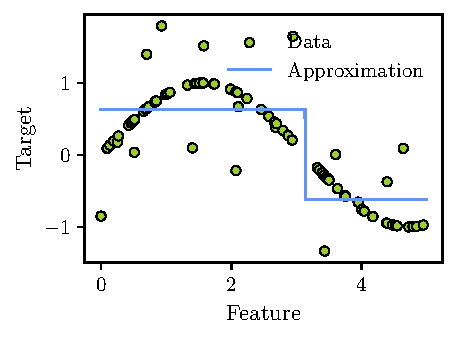
\includegraphics{decision-boundary-dt.pdf}
    \caption[Approximation of Decision Tree]{Approximation of a Decision Tree. A single split is performed at $\approx\num{3.1327505111694336}$ using the feature. All datapoints left respecitvely right of the split point share the region and are approximated by the region's response value.}
    \label{fig:decision-boundary-dt}
\end{figure}

So far, it remains open how the best split can be found. The best split is where the deviation between the prediction and the true response variable diminishes. For a single region, this error can be captured in the \gls{SSE} given by:
\begin{equation}
    \operatorname{L}_{\mathrm{SSE}} =\sum_{\mathbf{x}_{i} \in R_j}\left(y_{i}-\gamma_{j}\right)^{2},
\end{equation}
which is subsequently minimised \autocite[][231]{breimanClassificationRegressionTrees2017}. As documented in \textcite[][326]{hastietrevorElementsStatisticalLearning2009} we start with the entire dataset and scan through all combinations of features and possible split values. For a split by the feature $k$ at the value $s$, the child nodes are given by a pair of half-planes:
\begin{equation}
    R_1(k, s)=\left\{X \mid X_k \leq s\right\} \text { and } R_2(k, s)=\left\{X \mid X_k>s\right\}.
\end{equation}
Thereby, the feature $k$ and value $s$ are selected in a way, that the squared error in the child nodes is minimised:
\begin{equation}
    \min _{k, s}\left[\min _{\gamma_1} \sum_{\mathbf{x}_i \in R_1(k, s)}\left(y_i-\gamma_1\right)^2+\min _{\gamma_2} \sum_{\mathbf{x}_i \in R_2(k, s)}\left(y_i-\gamma_2\right)^2\right].
\end{equation}
Clearly, growing deeper trees leads to an improvement in the \gls{SSE}. Considering the extreme, where each sample has its region, the tree would achieve a perfect fit in-sample but perform poorly on out-of-sample data. To reduce the sensitivity of the tree to changes in the training data, hence \emph{variance}, size complexity pruning procedures are employed. Likewise, if the decision tree is too simplistic, a high bias contributes to the model's overall expected error. Both extremes are to be avoided.

Ensemble methods decrease the expected error of the decision tree by combining multiple trees in a single model through minimising the bias or variance term or both. Specifically, boosting addresses the bias and variance \autocites[][1672]{schapireBoostingMarginNew1998}[][29]{breimanRandomForests2001}. Next, we focus on \gls{GBRT}, a variant of boosting.

\subsubsection{Gradient Boosting
    Procedure}\label{sec:gradient-boosting-procedure}

Gradient boosting iteratively combines oversimplified models, the weak learners, into an additive model to obtain an improved ensemble estimate. This chapter draws on \textcite[][9]{friedmanGreedyFunctionApproximation2001} to derive gradient boosting for binary classification.

% classifier with outputs in [-1, 1]
By \cref{sec:problem-framing} we perform binary probabilistic classification and by \cref{sec:trade-initiator} we defined the labels to be $y \in \{-1,1\}$. For gradient boosting, instead of modelling the class-conditional probabilities directly, we model the conditional log odds instead, which can be interpreted as the probability of observing class $1$ or a buyer-initiated trade, and covert to class-conditional probabilities as needed.


\todo{better write logloss? Make connection clearer?}
Following \textcite[][9]{friedmanStochasticGradientBoosting2002} we set the loss function to be the cross-entropy loss, given by:
\begin{equation}
    L_{\mathrm{BCE}} \colon \mathbb{R}^2 \to \mathbb{R} \quad L_{\mathrm{BCE}}(y, F) = \log(1+\exp(-2yF))
    \label{eq:cross-entropy-loss}
\end{equation}
where:
\begin{equation}
    F(\mathbf{x}) = \frac{1}{2} \log \left[\frac{\Pr(y=1\mid \mathbf{x})}{\Pr(y=-1\mid \mathbf{x})}\right]
    \label{eq:logits-gbm}
\end{equation}
$F(\mathbf{x})$ is the model's prediction in terms of conditional log odds. The cross-entropy loss, is a reasonable choice, as it is suitable for binary classification, convex, and twice differentiable; properties we exploit later.

We first intialise the model with a naïve prediction, based on the average class $\bar{y}$ from all training samples:

\begin{equation}
    F_0(\mathbf{x})= \frac{1}{2} \log \left[\frac{1+\bar{y}}{1-\bar{y}}\right].
\end{equation}
Expectedly, $F_0(\mathbf{x})$ is a poor estimate, capturing hardly any regularities of the data. Gradient boosting solves this issue by adding weak learners to the ensemble. New trees are added greedily, one per iteration $m$ with $m=1,2,\cdots M$. The weak learner in the $m$-th iteration is chosen to approximate the pseudo residual $r_i$, which is the negative gradient of the observed value of the $i$-th sample and the current estimate:
\begin{equation}
    r_i=-\left[\frac{\partial L_{\mathrm{BCE}}\left(y_i, F\left(\mathbf{x}_i\right)\right)}{\partial F\left(\mathbf{x}_i\right)}\right]_{F(\mathbf{x})=F_{m-1}(\mathbf{x})}=2 y_i /\left(1+\exp \left(2 y_i F_{m-1}\left(\mathbf{x}_i\right)\right)\right).
\end{equation}
\todo{yields the maximum decrease are similar to the components of the negative gradient descent. However, the  major drawback is tha tthe gradient is only defined for data points xi seen during training, contradicting the creation of a generalising model.}
Typically, regression trees (cp. \cref{sec:decision-tree}) are chosen as weak learners since they are computationally cheap and can produce continuous estimates for the residual. The $m$-th regression tree contains $J$ terminal regions, denoted by $R_{j m}, j=1,2, \ldots, J_{m}$. We search for an estimate $\gamma_{j,m}$ for the terminal node $R_{jm}$ that minimises the cross-entropy over all samples within the node:
\begin{equation}
    \gamma_{j m}=\arg \min _\gamma \sum_{\mathbf{x}_i \in R_{j m}} \log \left(1+\exp \left(-2 y_i\left(F_{m-1}\left(\mathbf{x}_i\right)+\gamma\right)\right)\right)
    \label{eq:region-estimate-gbm}
\end{equation}

\cref{eq:region-estimate-gbm} cannot be solved in closed form and is typically approached by the Newton-Raphson method with a second-order approximation of the loss~\footnote{Compare the second-order Taylor polynomial given by \todo{complete?}.}:
\begin{equation}
    \gamma_{j m}=\sum_{\mathbf{x}_i \in R_{j m}} r_i / \sum_{\mathbf{x}_i \in R_{j m}}\left|r_i\right|\left(2-\left|r_i\right|\right)
\end{equation}
with $r_i$ given by \cref{eq:logits-gbm}.

An improved estimate for $\mathbf{x}$ is calculated from the previous estimate by adding the new regression tree to the ensemble. The latter moves the prediction towards the greatest descent and thus improves the overall prediction. The updated model is given by:
\begin{equation}
    F_{m}(\mathbf{x})=F_{m-1}(\mathbf{x})+\eta \sum_{j=1}^{J_{m}} \gamma_{j m} \mathbb{I}\left(\mathbf{x} \in R_{j m}\right).
\end{equation}
After $M$ iterations we obtain the final estimate calculated as $F_{M}\left(\mathbf{x}\right)$. To avoid \gls{overfitting} the residuals, only proportional steps towards the negative gradient are taken, which is controlled by the learning rate \eta~\autocite[][13]{friedmanGreedyFunctionApproximation2001}. The learning rate \eta~and the size of the ensemble $M$ are deeply intertwined and best tuned together \autocite[][13]{friedmanGreedyFunctionApproximation2001}.

Gradient boosting is still prone to \gls{overfitting} due to fitting trees to point-wise gradients. One solution is to employ early stopping, whereby the ensemble is only grown in size, as long as adding more weak learners leads to a decrease in loss on the validation set \autocite[][384]{hastietrevorElementsStatisticalLearning2009}. Another approach is to limit the amount of data seen during training by fitting trees on random subset of samples, as proposed in \textcite[][3]{friedmanStochasticGradientBoosting2002}, or on a subset of features, as popularised by \textcite[][3]{chenXGBoostScalableTree2016}. \textcite[][6]{prokhorenkovaCatBoostUnbiasedBoosting2018} grow oblivious trees, which use the same splitting criterion for all nodes of one level in a tree. The rationale is, that these arguably simplistic trees, and achieve an imperfect fit, which regularises the model. Finally, the loss function can be extended for a $\ell_2$ regularisation term to penalise the model for complexity \autocite[][2]{chenXGBoostScalableTree2016}.

In recent years, several variants of gradient boosting have been proposed and studied in the literature, including CatBoost \autocite[][1--23]{prokhorenkovaCatBoostUnbiasedBoosting2018}, XGBoost \autocite[][1--13]{chenXGBoostScalableTree2016}, and LightGBM \autocite[][3]{keLightGBMHighlyEfficient2017}, which differ by the policy how trees are grown and how \gls{overfitting} is addressed. Performance-wise, differences between the implementations are negligible, as empirical studies suggest \autocites[][8]{grinsztajnWhyTreebasedModels2022}[][19--20]{gorishniyRevisitingDeepLearning2021}[][7]{somepalliSaintImprovedNeural2021}[][14]{borisovDeepNeuralNetworks2022}.

As we noted at the beginning, $F_M(\mathbf{x})$ models the log odds. We can recover the class-conditional probabilities $\widehat{\operatorname{Pr}}(y \mid \mathbf{x})$ by taking the inverse:
\begin{equation}
    \widehat{\operatorname{Pr}}(y \mid \mathbf{x}) = 1 /\left(1+\exp(-2yF_M(\mathbf{x}))\right).
\end{equation}
and get the most probable class by \cref{eq:class-from-prob}.

\subsection{Transformer Networks}\label{sec:transformer-networks}

The subsequent chapters provide an introduction to classifiers based on the Transformer architecture.

\subsubsection{Architectural Overview}\label{sec:architectural-overview}

The Transformer is a neural network architecture by \textcite[][2--6]{vaswaniAttentionAllYou2017} proposed for sequence-to-sequence modelling. Its original application is in machine translation, whereby sentences in the source language are translated into sentences in the target language. More precisely, the sentence is first decomposed into individual \glspl{token} and mapped into a sequence of \glspl{embedding}, which are rich vector representations of the raw input. The Transformer then processes the \glspl{embedding} to generate the output sequence.

As the network operates on \glspl{embedding}, rather than strings, the architecture is not constrained to process textual data. It has been adapted to other modalities including image data \autocites[][2--5]{parmarImageTransformer2018}[][3]{dosovitskiyImageWorth16x162021} and tabular data \autocite[cp.][4]{gorishniyRevisitingDeepLearning2021}. The latter is important for our work, as derived in \cref{sec:selection-of-approaches}.

Following the architecture for machine translation of \textcite[][3]{sutskeverSequenceSequenceLearning2014}, the network features two main components: the encoder and the decoder. A sequence of \glspl{token} is first mapped to a sequence of \glspl{embedding} and augmented with positional information. The encoder receives these \glspl{embedding} and creates an enriched representation from it by encoding the context in which the input appears i.e., the surrounding words. The output of the encoder is then fed to the decoder. The decoder takes the embedded target sequence along with parts of the encoded representation of the input, to autoregressively generate the output sequence, i.e., the translation in the target language \gls{token} by \gls{token} \autocite[][3]{vaswaniAttentionAllYou2017}. \cref{fig:transformer-architecture-overview} depicts the complete architecture and serves as a guide through the subsequent sub-chapters.

The encoder consists of $\gls{L}=6$ stacked Transformer blocks \autocite[][6]{vaswaniAttentionAllYou2017}. Each block itself is composed of two sub-layers: a multi-head self-attention layer, followed by a position-wise, \gls{feed-forward-network}. Both components serve a distinct purpose in the Transformer. The self-attention mechanism encodes the context in which the input appears onto the \glspl{embedding}, whereas the \gls{feed-forward-network} serves as a long-term memory persisting information outside the immediate context. In the multi-head self-attention mechanism of the encoder, inputs can learn from any \gls{token} of the input sequence, even if a \gls{token} appears causally before the other input. Each of the sub-layers is surrounded by skip connections \autocite[][2]{heDeepResidualLearning2015} and followed by layer normalisation \autocite[][4]{baLayerNormalization2016} to facilitate and stabilise training. Stacking multiple Transformer blocks enables the model to learn hierarchical features from the inputs and targets. Applied to language processing, the first layers in the stack extract coarse-grained syntactic features, and subsequent layers learn fine-grained semantic features \autocites[][3651]{jawaharWhatDoesBERT2019}[][4596]{tenneyBERTRediscoversClassical2019}. For tabular data, this translates to frequent feature combinations or infrequent feature interactions.

Aside from the feed-forward sub-layer, the decoder contains a sub-layer for multi-head self-attention on the output of the encoder, known as cross-attention, and a masked variant of the multi-head self-attention for use on the output sequence. Here, causal masking enforces the autoregressive properties of the decoder.

The output of the decoder is finally passed through a linear layer with a softmax activation function to unembed the output and retrieve the probabilities of the next \gls{token} \autocite[][5]{vaswaniAttentionAllYou2017}. Since the output sequence is generated autoregressively, the most probable \gls{token} is fed back as input to the decoder to provide context for the following \glspl{token} until the remaining sequence is generated.

For its original application, machine translation, both the encoder and decoder are used. Yet, the modular design allows adapting Transformers to a wider range of use cases, some of which only require the encoder or decoder. \textcite[][16--17]{raffelExploringLimitsTransfer2020} differentiate these modes: encoder-only architecture, which encodes the input to obtain an enriched representation, decoder-only architectures to generate new \glspl{token} and encoder-decoder models for sequence-to-sequence modelling autoregressively. As our focus is on the probabilistic classification of tabular data, the goal is to learn an enriched representation of the input for classifying the label, here $\gls{y}$, rather than generating new samples. As such, encoder-only Transformers suffice. This insight also guides the structure in the next chapters, which focus on \glspl{embedding} and the inner workings of the encoder.

\begin{landscape}
    \begin{figure}[ht]
        \centering
        {\renewcommand\normalsize{\scriptsize}%
            \normalsize
            \input{./Graphs/transformer-architecture.pdf_tex}}
        \caption[Overview Over the Transformer Architecture]{Overview over the Transformer Architecture. The left part shows the self-attention mechanism discussed in \cref{sec:attention}. The central part depicts the multi-head self-attention mechanism, as covered in \cref{sec:attention}. The right part shows the encoder and decoder stack, as well as the \gls{embedding} mechanism as covered in \cref{sec:token-embeddings} onwards. Own work inspired by \textcite[][3]{tayEfficientTransformersSurvey2022}.}
        \label{fig:transformer-architecture-overview}
    \end{figure}
\end{landscape}

\subsubsection{Token Embedding}\label{sec:token-embeddings}

As explained previously, Transformers operate on sequences of numeric vector representations, the \emph{token embeddings}. The classical Transformer was trained on \emph{word embeddings}. Nevertheless, \gls{token} embeddings are generic and arbitrary inputs that can be embedded and then processed by the Transformer. In the spirit of \textcite[][5]{vaswaniAttentionAllYou2017}, we first explore word embeddings for textual data, before adapting embeddings to the tabular domain.

\todo{write down, how sequence of token ids is constructed.}

\textbf{Embeddings For Textual Data}

To obtain \gls{token} embeddings from the raw input sequences i.e., a sentence, the sequence is first split into constituent vocabulary elements, the \emph{tokens}. All known \glspl{token} are stored in a vocabulary. The vocabulary $V$ consists of $N_{V}=|V|$ elements and maps \glspl{token} onto their unique integer keys, referred to as \emph{token-ids} \autocite[][3]{phuongFormalAlgorithmsTransformers2022}. Apart from \glspl{token} in the training corpus, the vocabulary may include special \glspl{token}, like the $\mathtt{[UNK]}$ \gls{token} to handle out-of-vocabulary items or $\mathtt{[CLS]}$ \gls{token} for storing an aggregate representation of the sequence for classification \autocite[cp.][4]{devlinBERTPretrainingDeep2019}.

For ease of explanation, we equate \glspl{token} with words.\footnote{There is a subtle difference between \glspl{token} and words. A \gls{token} can be words including punctuation marks. But words can also be split into multiple \glspl{token}, such as sub-words \autocite[][3]{bojanowskiEnrichingWordVectors2017} or characters. To decrease the size of the vocabulary, words may be reduced to their stems, lower-cased, and stop words be removed.} Consider the following example with a small vocabulary of $V=\left\{1, N_v\right\}$ and a mapping between the \gls{token} and token-id of $\mathrm{'queen'}\mapsto 1$; $\mathrm{'king'}\mapsto 2$. For the sample sequence »Kings and Queens«, the sequence of token-ids is $\mathbf{s}=[2, 1]$, after applying tokenizing by words and common pre-processing like lower-casing, and the removal of the stop word »and«. Arbitrary sequences are given by $\mathbf{s} \equiv s[1: \ell] \equiv$ $s[1] s[2] \ldots s[\ell] \in V^*$.

The conversion to token-ids, however, loses the semantics, as token-ids may be assigned arbitrarily or ordering by semantics may not be feasible. This limitation can be overcome by embeddings, as pioneered by \textcite[][1139]{bengioNeuralProbabilisticLanguage}, which map each token-id into a high-dimensional space. By representing words as a vector, semantic and syntactic relationships between tokens can be encoded. As such, related words share a similar embedding vector \autocite[][1139]{bengioNeuralProbabilisticLanguage}. Moreover, word embeddings are semantically meaningful and can capture linguistic regularities, like gender through offsets between vectors \autocite[][748--749]{mikolovLinguisticRegularitiesContinuous2013}.

The embedding layer from \cref{fig:transformer-architecture-overview} is ultimately a lookup table to retrieve the embedding vector $\gls{e} \in \mathbb{R}^{d_{e}}$ from a learnt embedding matrix $\gls{W-e} \in \mathbb{R}^{d_{e} \times N_{V}}$ with the token-id $v \in V \cong\left[N_{V}\right]$ as shown:\footnote{Throughout our discussion on Transformers we adopt a notation proposed in \textcite[][1--16]{phuongFormalAlgorithmsTransformers2022}.}
\begin{equation}
    \gls{e}=\gls{W-e}\left[:, v\right].
    \label{eq:word-embeddings}
\end{equation}
The weights of $\gls{W-e}$ are initialised randomly and updated using gradient descent to obtain the learnt embeddings. The dimension of the embedding $d_e$ affects the expressiveness of the network and is thus an important tuneable hyperparameter of the model. All embeddings of the input sequence are finally gathered in a matrix $\mathbf{S} \in \mathbb{R}^{d_e \times \ell_s}$.

Concluding the example from above with artificial embeddings of $d_e=3$:
\begin{equation}
    \begin{aligned}
        \gls{e}_{\mathrm{king}}  & =\gls{W-e}\left[:,2\right] = [0.01, 0.20, 0.13]^{\top} \\
        \gls{e}_{\mathrm{queen}} & =\gls{W-e}\left[:,1\right] = [0.07, 0.16, 0.14]^{\top} \\
    \end{aligned}
\end{equation}
are likely to be close in embedding space with cosine-similarity of $\approx 1$ due to their high semantic similarity.

As this work is concerned with the classification of tabular data, the aforementioned concepts must be evolved. Differently from textual data, where all tokens come from the same vocabulary and a homogeneous embedding procedure suffices, tabular data is flexible regarding the columns, their data type, and their semantics. Only a shared meaning across rows can be assumed. For instance, every sample in a trade dataset may contain the previous trade price, yet the meaning of the trade price is different from other columns, urging the need for heterogeneous embeddings. Additionally, columns may be categorical or numerical.

\textbf{Embeddings For Numerical Data}

Transformer networks can handle numerical features, such as the trade price, by mapping the scalar value to a high-dimensional embedding vector and process sequences thereof \autocite[][3]{gorishniyEmbeddingsNumericalFeatures2022}. In the simplest case, a learnt linear projection is utilised to obtain the embedding. Linear embeddings of numerical features were previously explored in \textcites[][3]{kossenSelfAttentionDatapointsGoing2021}[][4]{somepalliSaintImprovedNeural2021}[][4]{gorishniyRevisitingDeepLearning2021}.

In analogon to the word case, if the $m$-th feature, $\mathbf{x}[m]$, is numerical, it is projected to its embedding $\gls{e} \in \mathbb{R}^{d_e}$ by element-wise multiplication with a learnt vector $\mathbf{W}_m \in \mathbb{R}^{d_{e}}$. Moreover, a feature-dependent bias term $\mathbf{b}_m \in \mathbb{R}^{d_{e}}$ is added, as noted in \cref{eq:numerical-embeddings}.
\begin{equation}
    \gls{e}= \mathbf{W}_m \mathbf{x}[m] +\mathbf{b}_m
    \label{eq:numerical-embeddings}
\end{equation}
More sophisticated approaches rely on parametric embeddings, like the \emph{piece-wise linear encoding} or the \emph{periodic encoding} of \textcite[][10]{gorishniyEmbeddingsNumericalFeatures2022}. Both enforce non-linearity. The authors show that these can alleviate the model's performance but at a non-neglectable computational cost. For this reason, our focus is on the computational more tractable linear embedding.

More generally, the works of \textcites[][1]{gorishniyEmbeddingsNumericalFeatures2022}[][1]{somepalliSaintImprovedNeural2021} suggest, that numerical embedding can significantly improve robustness to missing values or noise. Their work miss a theoretical explanation. \textcite[][8--9]{grinsztajnWhyTreebasedModels2022} fill this void and attribute the increased robustness to the broken rotational invariance.

\textbf{Embeddings For Categorical Data}

Datasets often comprise categorical features like the underlying. In the context of tabular Transformers, learnt categorical embeddings are widely used, which are similar to the word embedding
\autocites[][4]{gorishniyRevisitingDeepLearning2021}[][2]{huangTabTransformerTabularData2020}[][4]{somepalliSaintImprovedNeural2021}. Analogous, each category is mapped to an embedding vector using a learnt embedding matrix. Due to the heterogeneous nature of tabular data, embeddings may not be shared between features.

For categorical inputs, the embedding is implemented as a lookup table, analogous to \cref{eq:word-embeddings}. However, each feature has
its vocabulary $C_t$ with $N_{C_m}$ categories. Assume, the $m$-th feature is categorical. The specific embeddings $\gls{e}$ are queried with a unique integer key $c_{m} \in C_m \cong\left[N_{C_t}\right]$ from the learnt embedding matrix $\mathbf{W}_m \in \mathbb{R}^{d_e \times N_{C_m}}$. Finally, a feature-specific bias term $\mathbf{b}_m \in \mathbb{R}^{d_{e}}$ is added as shown in \cref{eq:categorical-embeddings}. Like for the word case, all embeddings of an instance are gathered in $\mathbf{S}$.
\begin{equation}
    \gls{e}=\mathbf{W}_m[:,c_{m}] +\mathbf{b}_m
    \label{eq:categorical-embeddings}
\end{equation}
These categorical embeddings can potentially capture the intrinsic properties of categorical variables by arranging similar categories closer in the embedding space. For instance, consider the underlyings $\mathtt{GOOGL}$ (Alphabet Inc.), $\mathtt{MSFT}$ (Microsoft Inc.), and $\mathtt{K}$ (Kellogg Company). Due to the overlapping field of operations, one would anticipate greater similarity between Alphabet and Microsoft.

Despite these advantages, high-cardinal features present a challenge for embeddings since they are typically learnt from a few samples, which promotes \gls{overfitting}. Handling high-dimensional categorical data remains an open research problem, as noted by \textcite[][2]{borisovDeepNeuralNetworks2022}.

\textbf{Link To Positional Encoding and Attention}

\todo{verify invariant property. Not sure if I got it right.}
Embeddings can only encode the semantic relationship of tokens, but they do not provide a clue to the model about the relative and absolute ordering of tokens in which they appear in the sequence, since all stages of the encoder and decoder are invariant to the token's position. Positional information must be induced into the model to preserve the ordering (cp. \cref{sec:positional-encoding}). Another limitation of embeddings is, that identical tokens share the embedding, even if they are ambiguous and their meaning is different from the context in which they appear. To resolve this issue, embeddings get contextualised in the self-attention mechanism (cp. \cref{sec:attention}).

\subsubsection{Positional Encoding}\label{sec:positional-encoding}

In practice, the order of words is important for the overall meaning of a sentence. As such, \textcite[][6]{vaswaniAttentionAllYou2017} propose to inject information on the \gls{token}'s position within the sequence through a \emph{positional encoding}, that is added onto the \gls{token} embedding.

Contrary to sentences, columns in tabular datasets are arranged in an arbitrary order, which weakens the need for positional information. However, unless the embeddings per feature are unique, a positional embedding is also required so that the model can relate the otherwise identical embeddings to specific features and distinguish them \autocites[][3]{huangTabTransformerTabularData2020}[][15]{somepalliSaintImprovedNeural2021}.

Like \gls{token} embeddings, positional embeddings can also be learnt \autocite[cp.][4174]{devlinBERTPretrainingDeep2019}. Due to better, extrapolation capabilities, \textcite[][6]{vaswaniAttentionAllYou2017}, propose an positional encoding with the mapping $\gls{W-p}: \mathbb{N} \rightarrow \mathbb{R}^{d_{e}}$ based on sine and cosine signals to encode the \emph{absolute} position of the \gls{token}:
\begin{equation}
    \begin{aligned}
        \gls{W-p}\left[2 i-1, t\right] & =\sin \left(t / \gls{ellmax}^{2 i / \gls{d}_e}\right), \\
        \gls{W-p}\left[2 i, t\right]   & =\cos \left(t / \gls{ellmax}^{2 i / \gls{d}_e}\right).
    \end{aligned}
    \label{eq:sinusodal-encoding}
\end{equation}
with $0<i \leq \gls{d}_{e} / 2$, the maximum sequence length $\gls{ellmax}$, which is arbitrarily set to $\gls{ellmax}=\num{10000}$, and $\gls{t}$ is again the position of the \gls{token} in the sequence. As shown in \cref{eq:sinusodal-encoding} the frequency decreases across the position dimension and alternates between sine and cosine for the embedding dimension. Each embedding thus contains a pattern, easily distinguishable by the model.

\begin{figure}[ht]
    \centering
    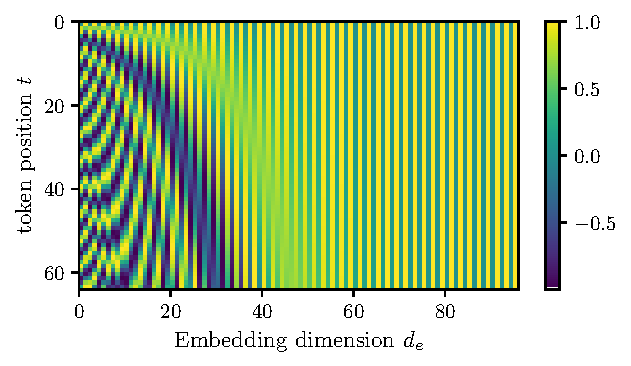
\includegraphics{positional-encoding.pdf}
    \caption[Positional Encoding of Transformer]{Positional encoding. The encoding is added onto the \gls{token} embeddings to infer positional information. The heatmap visualises the uniquely identifying pattern created from sine and cosine signals at increasing frequencies across the embedding dimension.}
    \label{fig:positional-embedding}
\end{figure}

The positional encoding is visualised in \cref{fig:positional-embedding}. One can see the alternating pattern between even and odd columns and the unique pattern for each \gls{token}'s position.

Using trigonometric functions for the positional embedding is favourable, due to being zero-centred and resulting in values in the closed range of $[-1,1]$. These properties are long known to promote convergence of neural networks \autocites[][8-9]{lecunEfficientBackProp2012}[][2]{ioffeBatchNormalizationAccelerating2015}.

The reason for encoding with both the sine and cosine is more subtle, as either one would suffice for absolute embeddings. \textcite[][6]{vaswaniAttentionAllYou2017} hypothesise, that besides learning the \emph{absolute} position i.e., fifth place in sequence, providing both sine and cosine also enables the model to attend to \emph{relative} positions, i.e., two places from a given \gls{token}.

The positional embedding is finally added per element to the token embedding to form a \gls{token}'s initial embedding $\gls{e}$. For the $\gls{t}$-th \gls{token} of a sequence $\mathbf{s}$, the embedding becomes:
\begin{equation}
    \gls{e}=\gls{W-e}\left[:, s[t]\right]+\gls{W-p}\left[:, t\right].
    \label{eq:positional-embedding}
\end{equation}
Intuitionally, adding the positional encoding leads to a rotation of the \gls{token} embedding in the embedding space. As the positional embedding is different for every location within the sequence, otherwise identical \glspl{token}, now have a distinct embedding.

\subsubsection{Attention Mechanism}\label{sec:attention}

Recall from our discussion on token embeddings, that embeddings are not yet context-sensitive. The Transformer relies on an \emph{attention mechanism} to let tokens gather information from other tokens within the sequence and thereby encode the context onto the embeddings.

\textbf{Preliminaries}

Attention can be thought of as a mapping between a query and a set of key-value pairs to an output. In general, the current token is first projected onto a query vector, and all tokens in the context are mapped to key and value vectors. Similar to a soft dictionary lookup, the goal is to retrieve the values from tokens in the context for which the keys are similar to the query and return an aggregate estimate of the values weighted by the similarity of the keys and the query. Naturally, if a token in the context is important for predicting the queried token, indicated by a high similarity, the value of the context token has a large contribution to the output \autocites[][5]{phuongFormalAlgorithmsTransformers2022}[][3]{vaswaniAttentionAllYou2017}.

Attention first appeared in \textcite[][4]{bahdanauNeuralMachineTranslation2016} and was popularised by \textcite[][4]{vaswaniAttentionAllYou2017}. The latter introduced a specific attention mechanism, known as \emph{scaled dot-product attention}, which we introduce in detail.

\textbf{Scaled Dot-Product Attention}

Analogous to before, \emph{scaled dot-product attention} estimates the similarity between queries and keys, as the dot product. The resulting attention scores are divided by some constant and normalised using a softmax function to obtain the attention weights. Multiplication of the attention weights with the values yields the outputs. Scaled dot-product attention is visualised in \cref{fig:transformer-architecture-overview} (left).

For computational efficiency, attention is performed simultaneously over multiple queries. Thus, the author's group queries, keys, and values in matrices. In matrix notation outputs are estimated as:

\begin{equation}
    \begin{aligned}
        \operatorname{Attention}(\mathbf{S},\mathbf{Z}) & = \mathbf{V} \operatorname{softmax}\left(\mathbf{A} / \sqrt{d_{\mathrm{attn}}}\right) \\
        \mathbf{A}                                      & = \mathbf{K}^{\top} \mathbf{Q}
    \end{aligned}
    \label{eq:attention}
\end{equation}
where $\mathbf{S} \in \mathbb{R}^{d_s \times \ell_s}$ and $\mathbf{Z} \in \mathbb{R}^{d_z \times \ell_z}$ are vector representations of the primary input sequence and of the context sequence. Both the primary and the context sequences are identical for the encoder but are different for the decoder. The query, key, and value matrices $\mathbf{Q}=\mathbf{W}_q \mathbf{S} + \mathbf{b}_q\mathbf{1}^{\top}$, $\mathbf{K}=\mathbf{W}_k \mathbf{Z} + \mathbf{b}_k\mathbf{1}^{\top}$, and $\mathbf{V}=\mathbf{W}_v \mathbf{Z} + \mathbf{b}_v\mathbf{1}^{\top}$ are linear projections of the input and context sequences, and $\mathbf{W}_q, \mathbf{W}_k \in \mathbb{R}^{d_{\mathrm{attn}\times d_{s}}}$; $\mathbf{W}_v \in \mathbb{R}^{d_{\mathrm{out}\times d_{z}}}$; $\mathbf{b}_q, \mathbf{b}_k \in \mathbb{R}^{d_{\mathrm{attn}}}$, and $\mathbf{b}_v \in \mathbb{R}^{d_{\mathrm{out}}}$ are learnable parameters. The dimensionality of the attention mechanism, $d_{\mathrm{attn}}$, is typically a fraction of the model dimensionality to accelerate computation. Likewise, the output dimension, $d_{out}$, is another hyperparameter to the models. The attention scores are $\mathbf{A}$, which are scaled by $\sqrt{d_{\mathrm{attn}}}$ to avoid unstable gradients, and the softmax activation normalises all scores. As normalised attention scores have a clear interpretation as the weights of how much a token contributes to the model's output, the attention mechanism provides a window into the model, which we explore in \cref{sec:feature-importance-measure}.

\textbf{Multi-Head Attention}

Rather than relying on a single attention function, \textcite[][4--5]{vaswaniAttentionAllYou2017} introduce multiple \emph{attention heads}, which perform attention in parallel on $H$ \emph{different} linear projections of queries, keys, and values. The \emph{multi-head attention} enables the model to learn richer representations of the input, as attention heads operate independently, they can pick up unique patterns or focus on different positions in the sequence at once. Multi-head attention is visualised in \cref{fig:transformer-architecture-overview} (centre).

\todo{introduce word modalities}
Exemplary for machine translation, \textcite[][5795]{voitaAnalyzingMultiHeadSelfAttention2019} show, that heads serve indeed distinct purposes like learning positional or syntactic relations between tokens. It is conceivable, that for tabular data this maps to dependencies between features. In practice, Transformers may not leverage all attention heads and some heads could even be pruned without impacting the performance \autocites[][9]{michelAreSixteenHeads2019}[][5805]{voitaAnalyzingMultiHeadSelfAttention2019}.

Multi-head attention can be computed as:

\begin{equation}
    \begin{aligned}
        \operatorname{MHAttention}(\mathbf{S}, \mathbf{Z}) & = \mathbf{W}_{o}\left[\mathbf{Y}^{1};\mathbf{Y}^{2};\ldots;\mathbf{Y}^{H} \right] + \mathbf{b}_{o}\mathbf{1}^{\top} \\
        \mathbf{Y}^{h}                                     & = \operatorname{Attention}(\mathbf{Q}^h, \mathbf{K}^h, \mathbf{V}^h)
    \end{aligned}
\end{equation}
The query, key, and value matrices  $\mathbf{Q}^{h}=\mathbf{W}^h_q \mathbf{S} + \mathbf{b}^h_q\mathbf{1}^{\top}$, $\mathbf{K}^{h}=\mathbf{W}_k^h \mathbf{Z} + \mathbf{b}_k^h\mathbf{1}^{\top}$, and $\mathbf{V}^{h}=\mathbf{W}_v^h \mathbf{Z} + \mathbf{b}_v^h\mathbf{1}^{\top}$ are obtained from linear projections of the input and context sequences unique per head. Again, $\mathbf{W}^{h}_{q} \in \mathbb{R}^{d_{\mathrm{attn}}\times d_{S}}$; $\mathbf{W}^{h}_{k}, \mathbf{W}^{h}_{v} \in \mathbb{R}^{d_{\mathrm{attn}}\times d_z}$; $\mathbf{b}^h_q, \mathbf{b}^h_k \in \mathbb{R}^{d_{\mathrm{attn}}}$, and $\mathbf{b}^h_v \in \mathbb{R}^{d_{\mathrm{mid}}}$ are used for projection. Typically, the dimensionality of the attention heads, $d_{\mathrm{mid}}$, is reduced to $d_{\mathrm{attn}}/H$ to match the computational cost of single-head attention. The output dimensionality $d_{\mathrm{out}}$ is restored with a final linear projection through the weight matrix $\mathbf{W}_{o} \in \mathbb{R}^{d_{\mathrm{out}}\times Hd_{\mathrm{mid}}}$ and bias $\mathbf{b}_o \in \mathbb{R}^{d_{\mathrm{out}}}$ applied to the concatenated results of the attention heads.

The concatenated and projected output of the attention heads is then passed to the point-wise feed-forward networks, which enables interaction between the head's outputs. We discuss position-wise feed-forward networks in \cref{sec:position-wise-ffn}.

\textbf{Masked Self-Attention and Cross-Attention}

In the \cref{eq:attention}, tokens can attend to any preceding or subsequent token without restrictions. Thus, the full \emph{bidirectional context} is used. This design is optimal for the encoder, where the entire input sequence shall serve as the context.

For the decoder, the self-attention is modified to \emph{masked self-attention} and \emph{cross-attention} mechanism. First, causal masking is required to achieve autoregressive sequence generation in the decoder. The context is \emph{unidirectional}, where a token is only allowed to attend to itself or all previously generated tokens. Second, the decoder uses \emph{cross-attention} to connect between the encoder and decoder. Other than in the self-attention mechanism, where keys, values and queries are generated from the same sequence, keys and values come from the encoder and queries are provided by the decoder. As our focus is on encoder-only architectures, we refer the reader to \textcite[][16--17]{raffelExploringLimitsTransfer2020} for an in-depth treatment of both topics.

\subsubsection{Position-Wise Feed-Forward Networks}\label{sec:position-wise-ffn}

The attention mechanism enables \glspl{token} to attend to other inputs in the immediate context. To retain general information on the task, outside and independent of the immediate context, each Transformer block adds a point-wise \gls{feed-forward-network}, which acts as a persistent memory to the model \autocite[][3]{sukhbaatarAugmentingSelfattentionPersistent2019}.

The network consists of a linear transformation, followed by a non-linear activation function and a second linear layer. For the $l$-th layer, the \gls{MLP} is given by
\begin{equation}
    \mathbf{S} = \mathbf{S}+\mathbf{W}_{\mathrm{mlp} 2}^l \operatorname{ReLU}\left(\mathbf{W}_{\mathrm{mlp} 1}^l \mathbf{S}+\mathbf{b}_{\mathrm{mlp} 1}^l 1^{\top}\right)+\mathbf{b}_{\mathrm{mlp} 2}^l 1^{\top},
\end{equation}
with $\mathbf{W}_{\mathrm{mlp} 1}^l \in \mathbb{R}^{d_{\mathrm{mlp}} \times d_{e}}, \mathbf{b}_{\mathrm{mlp} 1}^l \in \mathbb{R}^{d_{\mathrm{mlp}}}, \mathbf{W}_{\mathrm{mlp} 2}^l \in \mathbb{R}^{d_{e}} \times d_{\mathrm{mlp}}$ and $\mathbf{b}_{\mathrm{mlp} 2}^l \in \mathbb{R}^{d_{e}}$ being learnable parameters identical for all \glspl{embedding} in the layer. The network is applied to each embedding separately and identically.

\textcite[][9]{vaswaniAttentionAllYou2017} set the hidden dimension to be two to eight magnitudes of the embedding dimension. The large capacity strengthens the model's ability to retain information but also contributes significantly to the high computational requirements and memory footprint of Transformers \autocites[][5]{tayEfficientTransformersSurvey2022}[][1]{kitaevReformerEfficientTransformer2020}. Both linear transformations are separated by a \gls{ReLU} \gls{activation-function} \autocite[][318]{glorotDeepSparseRectifier2011} to introduce non-linearities to the network.

Like the attention layer, the position-wise \gls{FFN} is surrounded by residual connections, followed by layer normalisation (cp. \cref{sec:residual-connections-layer-norm}). Both are vital for the training process and convergence of the overall network. Optionally, dropout \autocite[][1930]{srivastavaDropoutSimpleWay} is added to prevent the model from \gls{overfitting}.

\subsubsection{Residual Connections and Layer Normalisation}\label{sec:residual-connections-layer-norm}

Recall from earlier chapters, that the encoder stacks multiple Transformer blocks, each of which consists of several sub-layers, resulting in a deep network. While depth is inevitable to learn hierarchical representations, the training of such a network is complicated. As neural networks are commonly trained using backpropagation, which relies on the gradient of the error to be propagated through the network starting at the last layer, vanishing or \glspl{exploding-gradient} pose a major difficulty in training deep neural nets \autocite[][1]{heDeepResidualLearning2015}. Without countermeasures, stacking multiple layers in the encoder and decoder of the Transformers impedes the gradient information to flow efficiently through the network and hampers the training behaviour \autocite[][1811]{wangLearningDeepTransformer2019}.

As a remedy, \textcite[][3]{vaswaniAttentionAllYou2017} employ residual connections around each sub-layer, whereby the output of the sub-layer is added element-wisely to its input. Intuitively, the residual connection provides an alternative path for information to flow through the network, since some information can bypass the sub-layer and thereby reach deeper layers within the stack. Vanishing or \glspl{exploding-gradient} are also mitigated, as gradients can bypass the sub-layer, eventually contributing towards an easier optimisation \autocite[][3591]{liuRethinkingSkipConnection2020}. Residual connections moreover help to preserve the positional embeddings (cp. \cref{sec:positional-encoding}), as the layer's inputs are maintained in the identity mapping. Another technique to improve the training behaviour is layer normalisation.

\textcite[][3]{vaswaniAttentionAllYou2017} extensively draw on layer normalisation \autocite[][4]{baLayerNormalization2016} after the multi-head attention and feed-forward sub-layers. It is used for normalising the activations of the sub-layer and to stabilise and accelerate the training of the network \autocite[][2]{baLayerNormalization2016}. The normalisation statistics are calculated separately for every instance, which guarantees scalability across different batch sizes.

Until now it remains unclear, how the layer normalisation intertwines with the sub-layers and the residual connections. Transformers are distinguished by the order in which layer normalisation is added into the pre-norm and post-norm Transformer. Post-norm Transformers add layer normalisation to the sub-layer \emph{after} adding the input from the residual connections. The arrangement is depicted in \cref{fig:transformer-architecture-overview}. In contrast for pre-norm Transformers, the normalisation is applied \emph{before} the self-attention and feed-forward sub-layers and inside the residual connections. Pre-norm requires one additional normalisation layer to pass only well-conditioned outputs from the Transformer block to the successive layers \autocite[][5]{xiongLayerNormalizationTransformer2020}.

\textcite[][3]{vaswaniAttentionAllYou2017} employ post-layer normalisation, but recent research has shown a shift towards pre-norm setups \autocite[][4]{narangTransformerModificationsTransfer2021}. Parts of the widespread adaption lie in faster training and omitting of the need for costly learning rate warm-up stages, whereby the learning rate is initially decreased to keep the gradients balanced \autocites[][2]{xiongLayerNormalizationTransformer2020}[][8]{liuUnderstandingDifficultyTraining2020}. In addition, post-norm Transformers have been found brittle to train and prone to convergence failures with its root cause in vanishing gradients, \glspl{exploding-gradient}, and an overall higher dependency on the residual stream \autocites[][8]{liuUnderstandingDifficultyTraining2020}[][1812]{wangLearningDeepTransformer2019}. Pre-norm Transformers, although they may sacrifice some performance, introduce a certain robustness to the training process. We come back to this property in our discussion on the FT-Transformer.

\subsubsection{FT-Transformer}\label{sec:fttransformer}

\todo{try to introduce BERT here somewhere.}

Many of the previous concepts can be adapted to the tabular domain with minor architectural changes. \textcite[][5]{gorishniyRevisitingDeepLearning2021} propose with FT-Transformer an adaption, that pairs an embedding unit for both numerical and categorical inputs, dubbed the feature tokenizer, with a Transformer. The complete architecture is depicted in \cref{fig:fttransformer}. Notably, the Transformer units use a pre-norm setup for easier optimisation, whereby the very first normalisation layer in the encoder is removed due to a propitious performance \textcite[][17]{gorishniyRevisitingDeepLearning2021}. The upstream feature tokenizer transforms every feature in $\mathbf{x}$ to their embeddings. The embeddings are given by \cref{eq:numerical-embeddings,eq:categorical-embeddings}.

\begin{figure}[ht]
    \centering
    {\renewcommand\normalsize{\scriptsize}
        \normalsize
        \input{./Graphs/fttransformer.pdf_tex}}
    \caption[Overview Over the FT-Transformer Architecture]{Overview Over the Architecture of FT-Transformer. The FT-Transformer uses a pre-norm arrangement and operates on numerical and categorical embeddings. Own work inspired by \textcite[][4--5]{gorishniyRevisitingDeepLearning2021}.}
    \label{fig:fttransformer}
\end{figure}

Recall from our discussion on self-attention (cp. \cref{sec:attention}), that each \gls{token} encodes the \glspl{token} within the sequence. Based on this notion, \textcite[][4174]{devlinBERTPretrainingDeep2019} prepend a specialised $\mathtt{[CLS]}$ \gls{token} to the sequence, which stores the sequence's aggregate representation. Like any other \gls{token}, the $\mathtt{[CLS]}$ \gls{token} is embedded first and contextualised in the encoder. Its final hidden state is then used for classification.

\textcite[][4]{gorishniyRevisitingDeepLearning2021} adapt the idea of a $\mathtt{[CLS]}$ \gls{token} for tabular representation models. Similar to the embeddings of categorical or numerical features, the embedding of the $[\mathtt{CLS}]$ \gls{token} $\gls{e}_\mathtt{[CLS]} \in \mathbb{R}^{d_{e}}$ is prepended to the column embeddings with $\mathbf{S} = \left[\gls{e}_\mathtt{[CLS]}, \gls{e}_1, \ldots \gls{e}_{M}\right]$, where $\mathbf{S} \in \mathbb{R}^{d_{e} \times M +1}$. Like before, $\mathbf{S}$ is passed through a stack of Transformer layers. The updated representation of the $\mathtt{[CLS]}$ \gls{token} is used exclusively for prediction:
\begin{equation}
    P=\operatorname{Linear}\left(\operatorname{ReLU}\left(\operatorname{LayerNorm}\left(\mathbf{S}\left[:,0\right]\right)\right)\right).
    \label{eq:bert-ft}
\end{equation}
\todo{Add softmax, think about ReLU, change linear layer to Weight matrix?}

\textcite[][8]{gorishniyRevisitingDeepLearning2021} achieve state-of-the-art performance through numerical and categorical embeddings. Embedding both categorical and numerical inputs enables the Transformer to attend to all other features, but at considerable computational cost, that may only be justified by higher classification accuracies.

Next, all models are extended for learning on partially-labelled data.
\section{Semi-Supervised Approaches}\label{sec:semi-supervised-approaches}

This chapter expands the scope of trade classification from the supervised setting to the semi-supervised setting and presents suitable extensions.

\subsection{Framing as a Semi-supervised Learning Problem}\label{sec:problem-framing-2}

The supervised approaches depend on the availability of the trade initiator as the true label. Yet, obtaining the label is often restricted to the rare cases, where the trade initiator is provided by the exchange or to subsets of trades where the initiator can be inferred through matching procedures (cp. \cref{sec:trade-initiator}). This may bias the selection. Unlabeled trades, though, are abundant and can help improve the generalization performance of the classifier. This concern is addressed by semi-supervised methods.

Semi-supervised methods leverage partially-labeled data by learning an algorithm on unlabeled instances alongside true labels \autocite[\checkmark][2]{chapelleSemisupervisedLearning2006}. They are centered around the semi-supervised assumption of smoothness, which states that if two samples say $\mathbf{x}_{1}$ and $\mathbf{x}_{2}$ are nearby in a high-density region, their class labels $y_{1}$ and $y_{2}$ should also be similar. Vice versa, if data points are separated by a low-density region, their labels may be different \autocite[\checkmark][5]{chapelleSemisupervisedLearning2006}.

\begin{figure}[ht]
    \centering
    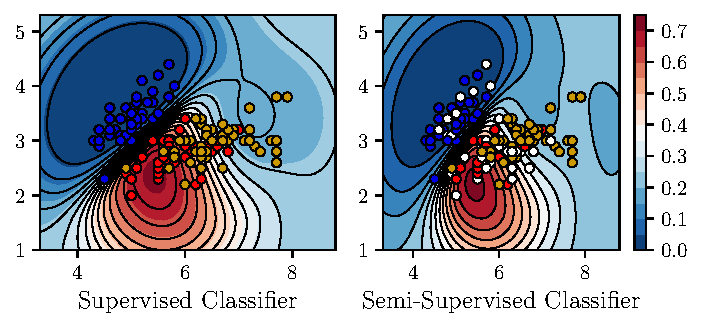
\includegraphics[width=0.8\linewidth]{decision-boundary-semi-supervised.pdf}
    \caption[Decision Boundary of Supervised and Semi-supervised Classifiers]{Decision boundary of a supervised and semi-supervised classifier. The supervised classifier is trained entirely on labeled data. The semi-supervised classifier uses both labeled and unlabeled instances to determine the decision boundary. Predicted class probabilities of \mycircle{viz-red} are visualized as a contour. Here, the unlabeled data points, drawn as \mycircle{viz-white}, lead to more confident predictions and a stretched class.}
    \label{fig:supervised-semi-supervised}
\end{figure}

Applied to trade classification, with semi-supervised methods we implicitly assume that trades with similar features, such as a common trade price and quotes, conform to the same class. The purpose of unlabeled trades is to help efficiently determine the boundary around regions of neighboring trades resulting in improved generalization performance. A visualization of a decision boundary of (semi-)supervised classifier is given in \cref{fig:supervised-semi-supervised}.

The semi-supervised setting requires extending our notation from \cref{sec:problem-framing}, by distinguishing between labeled and unlabeled instances. Like before, $\mathcal{D}=\left\{\left(\mathbf{x}_i, y_i\right)\right\}_{i=1}^N$ denotes all labeled trades. Unlabeled datapoints are stored in separate set $\mathcal{U} = \left\{\mathbf{x}_i\right\}_{i=1}^{K}$. Our coverage of semi-supervised approaches includes self-training for gradient boosting and pre-training of Transformers, which we derive from a subsequent discussion.

\subsection{Selection of Approaches}\label{sec:selection-of-approaches-1}

Our goal is to extend gradient-boosted trees and Transformers for the semi-supervised setting to make use of the abundant, unlabeled trade data. We are aimed to make minimally intrusive changes to maintain a fair comparison with the supervised counterparts. We find self-training for gradient boosting and pre-training of Transformers suitable for training on labeled and unlabeled trades, as our subsequent discussion derives.

\textbf{Gradient Boosting}

The success of supervised gradient boosting led to the development of gradient boosting for the semi-supervised setting. An early work of \textcite[\checkmark][555--556]{dalche-bucSemisupervisedMarginBoost2001} explores replacing supervised weak learners, i.e., regression trees, with semi-supervised weak learners, i.e., mixture models and minimizes a loss function over labeled and unlabeled instances. Another line of research, including \textcites[\checkmark][290--291]{bennettExploitingUnlabeledData2002}[\checkmark][2003--2004]{mallapragadaSemiBoostBoostingSemiSupervised2009}, retain supervised weak learners to generate pseudo labels of unlabeled instances per iteration. True labeled and pseudo-labeled data is then used in fitting weak learners of subsequent iterations. Approaches differ regarding the selection criterion of the pseudo-labeled instances. Both lines of work, however, require changes to the boosting procedure or the base learners.

An alternative is to pair gradient boosting with self-training. Self-training is a wrapper algorithm around a supervised classifier, that incorporates its most-confident predictions of unlabeled instances into the training procedure \autocite[\checkmark][190]{yarowskyUnsupervisedWordSense1995}. In contrast to previous methods, pseudo-labels are generated exclusively from the fully-fledged ensemble, which is grown multiple times at a higher computational cost. Being a model-agnostic wrapper, it does not change the classifier and ensures maximum comparability. This, together with the widespread adoption in the literature, makes it a compelling choice for semi-supervised trade classification.

\textbf{Transformer}

Whilst Transformers could be combined with self-training, a more promising approach is to pre-train Transformers on unlabeled data, and then fine-tune the network on the remaining labeled instances. Various studies report unanimously performance improvements from pre-training tabular Transformers, including \textcites[\checkmark][8]{somepalliSaintImprovedNeural2021}[\checkmark][7--8]{huangTabTransformerTabularData2020}.

Until now we assumed the parameters e.g., weights and biases, of the Transformer to be initialized randomly. The joint goal of pre-training objectives is to initialize a neural network with weights that capture expressive representations of the input and thereby improve generalization performance over a random initialization when fine-tuning on a specific task \autocite[\checkmark][636]{erhanWhyDoesUnsupervised}. The training is now decomposed into two stages: in the first stage the model is trained with respect to the pre-training objective to obtain the parameter estimates on unlabeled instances, and in the second stage the Transformer is initialized with the parameters and then finetuned on the labeled dataset. Particularly beneficial, general embeddings can be learned during pre-training, even if the true label, i.e., the trade initiator, is unknown or its definition varies between tasks.

Pre-training objectives for tabular data differ vastly in their methodology and are often directly adapted from other domains including \gls{MLM} \autocite[\checkmark][4174]{devlinBERTPretrainingDeep2019}, \gls{RTD} \autocite[\checkmark][2--3]{clarkElectraPretrainingText2020}, or contrastive learning \autocite[\checkmark][1598]{chenSimpleFrameworkContrastive2020}.
As such, \textcite[\checkmark][7]{huangTabTransformerTabularData2020} adapt \gls{MLM}, whereby features are randomly masked and the objective is to reconstruct the original input. Pre-training by \gls{RTD} aims to identify randomly replaced features and recover a binary mask used for replacement \autocite[\checkmark][7]{huangTabTransformerTabularData2020}. \textcites[\checkmark][3--4]{bahriSCARFSelfsupervisedContrastive2022}[][4--5]{yoonVIMEExtendingSuccess2020} reconstruct both the binary feature mask and the original input simultaneously. \textcite[\checkmark][3]{somepalliSaintImprovedNeural2021} alter the methodology of \textcite[\checkmark][11036--11037]{yoonVIMEExtendingSuccess2020} through a contrastive loss function.

With a multitude of methods, tested on different datasets and neural architectures, a fair comparison between pre-training methods is tedious. Yet, \textcite[\checkmark][2-3]{rubachevRevisitingPretrainingObjectives2022} provide guidance in selecting objectives. Among the pre-training objectives that they benchmark, the \gls{RTD} objective was among the best-performing approaches. The \gls{RTD} objective is easy to optimize, unsupervised, and leaves the model architecture unaltered, which makes \gls{RTD} a compelling choice for pre-training on unlabeled data.

The next chapter covers self-training in detail.

\subsection{Gradient Boosted Trees With Self-Training}\label{sec:extensions-to-gradient-boosted-trees}

Self-training is a wrapper algorithm around a probabilistic classifier, that incorporates its predictions of unlabeled instances as pseudo labels \autocite[\checkmark][190]{yarowskyUnsupervisedWordSense1995}.

Initially, a base classifier is fitted on the labeled data points in a supervised manner. The classifier then assigns labels, so-called pseudo labels, to unlabeled instances. A subset of unlabeled instances with high-confidence predictions is selected, removed from the unlabeled dataset and added to the pseudo-labeled data dataset. A new classifier is then retrained on the labeled and pseudo-labeled instances \autocite[\checkmark][190--192]{yarowskyUnsupervisedWordSense1995}. The process is repeated for several iterations until an abortion criterion applies, such as the maximum number of iterations is exhausted or when no unlabeled instances are left to label.

Recall from our discussion on gradient-boosted trees in \cref{sec:gradient-boosting-procedure} that we optimized for the cross-entropy loss on the training set. When coupled with self-training in each training iteration the classifier $F$ now jointly minimizes the loss over the labeled samples $\mathcal{D}$ and the pseudo-labeled samples $\not{\mathcal{U}}$:
\begin{equation}
    L_{\mathrm{ST}}=\frac{1}{\left|\mathcal{D}\right|} \sum_{(\mathbf{x}, y) \in \mathcal{D}} L(F(\mathbf{x}), y)+\frac{\epsilon}{\left|\not{\mathcal{U}}\right|} \sum_{(\mathbf{x}, \tilde{y}) \in \not{\mathcal{U}}} L(F(\mathbf{x}), \tilde{y})+\lambda\|F\|^2,
\end{equation}
where $\epsilon$ is a hyperparameter to control the impact of the pseudo-labeled data, $\tilde{y}$ is the pseudo-labeled instance, and $\lambda$ weights the regularization term \autocite[\checkmark][4]{aminiSelfTrainingSurvey2023}.

In every iteration, only unlabeled instances are added to the training set, for which the predicted class probability exceeds a confidence threshold, say $\tau$. This approach has implications, as highlighted by \textcite[\checkmark][32427]{chenDebiasedSelfTrainingSemiSupervised2022}. The threshold $\tau$ becomes an important hyperparameter in controlling that no noisy labels are added to the training set, but a restriction to highly-confidence samples may lead to a data bias and over-confidence in the prediction. Self-training is prone to a confirmation bias, as confident but wrong pseudo labels are erroneously incorporated into the training set, which in effect leads to a propagation of errors in the subsequent training rounds.

At the same time, self-training puts a high emphasis on the correctness of the probability estimates in the base classifier. This is problematic for decision trees, known to produce poor probability estimates, as probabilities are derived from the class frequency in the leaf node containing few samples \autocite[\checkmark][357--358]{tanhaSemisupervisedSelftrainingDecision2017}. However, as gradient boosting directly optimizes for the cross-entropy loss, the problem found for its ensemble member no longer occurs.

Independent of the base classifier, self-training increases computational cost, as training is repeated over several iterations on a growing training set \autocite[\checkmark][3841]{zophRethinkingPretrainingSelftraining2020}. Despite these limitations, the potentially improved decision boundary outweighs the concerns.

\subsection{Transformers With Pre-training}\label{sec:extensions-to-transformer}

\gls{RTD} is a pre-training objective proposed by \textcite[\checkmark][2--3]{clarkElectraPretrainingText2020} for the use in language models. The core idea is to randomly replace tokens with plausible alternatives and learn a binary classifier to distinguish between original and replaced tokens. Intuitionally, the random replacement forces the model to learn generalizable representations of the input, rather than memorizing the co-occurrence of certain tokens. Additionally, surprising the model with random tokens strengthens its ability to incorporate contextual information.

\begin{figure}[ht]
    \centering
    {\renewcommand\normalsize{\small}
        \normalsize
        \input{./Graphs/random-token-replacement.pdf_tex}}
    \caption[Replaced Token Detection]{Replaced Token Detection. Visualization inspired by \autocite[\checkmark][3]{clarkElectraPretrainingText2020}.}
    \label{fig:random-token-replacement}
\end{figure}

\todo{Adapt to tabular data}

The approach uses two neural networks, namely the generator and the discriminator, typically implemented as Transformers, as visualized in \cref{fig:random-token-replacement}.  The generator is responsible for generating replacement tokens and receives an input sequence, i.e., a sentence, that has been intentionally masked out. It learns to predict the original token of the now-masked token through tokens in the bidirectional context (cp. \cref{sec:attention}). For masking, an additional $\mathtt{[MASK]}$ token is introduced, which extends the vocabulary (cp. \cref{sec:token-embeddings}). Separately for each token, the final hidden state of the masked token is fed through a softmax activation to obtain the predicted probability distribution of the masked token and the cross entropy loss is used to compare against the true distribution. By replacing the masked token with a token from the generator distribution, convincing replacements now take place for some of the original inputs \autocite[\checkmark][2--3]{clarkElectraPretrainingText2020}.

The discriminator then receives the corrupted input sequence and is trained to distinguish between original and replaced tokens originating from the generator. The output is a binary mask to be compared against the mask initially used for masking tokens in the generator \autocite[\checkmark][2--3]{clarkElectraPretrainingText2020}.

Applied to tabular datasets, \gls{RTD} transfers to randomly replacing feature values in $\mathbf{x}_{i}$ instead of sequences. The objective is now to predict a binary mask $\mathbf{m}_{i}\in \{0,1\}^{M}$ corresponding to $\mathbf{x}_{i}$, indicating which features, or entries in $\mathbf{x}_{i}$, have been replaced. Previous adaptions for tabular data, e.g., \textcite[\checkmark][3]{huangTabTransformerTabularData2020}, simplify the replacement strategy by sampling replacement values directly from the feature, which alleviates the need for a generator network and requires less compute. Since the replacement is done on a feature-per-feature basis, the replaced token is \emph{per se} harder to detect.

For tabular the random replacement of feature values also strengthens the model's ability to incorporate a combination of features, rather than a single or few features based on their absolute value, which would facilitate overfitting.

In summary, \gls{RTD} can help to learn expressive representations of the input, even if the true label is unavailable. Given previous research, we expect pre-training \gls{RTD} to improve the performance of the FT-Transformer and match or exceed the of the \gls{GBRT}.
% \addtocontents{toc}{\protect\newpage}
\section{Empirical Study}\label{sec:empirical-study}

In this section, we demonstrate the efficacy of machine learning for trade classification in an empirical setting. We begin by outlining the dataset construction.

\subsection{Data and Data Preparation}\label{sec:data-and-data-preparation}

The following chapter describes the construction of datasets, that suffice the data requirements of classical trade classification rules and for our machine learning models. We also discuss how we define and infer the true trade initiator.

\subsubsection{Data Collection}\label{sec:data-collection}


Testing the empirical accuracy of our approaches requires option trades where the true initiator is known. To arrive at a labeled sample, we combine data from four individual data sources. Our primary source is LiveVol, which records option trades executed at US option exchanges at a transaction level. We limit our focus to option trades executed at the \gls{CBOE} and \gls{ISE}. LiveVol contains both trade and matching quote data. Like most proprietary data sources, it does not distinguish the initiator nor does it include the involved trader types. For the \gls{CBOE} and \gls{ISE} exchange, the \gls{ISE} Open/Close Trade Profile and \gls{CBOE} Open-Close Volume Summary contain the buy and sell volumes for the option series by trader type aggregated on a daily level. A combination of the LiveVol dataset with the open/close data, allows us to infer the trade initiator for a subset of trades. For evaluation and use in some of our machine learning models, we acquire additional underlying and option characteristics from IvyDB's OptionMetrics.

In \cref{sec:trade-initiator} we discussed three views on the trade initiator. Due to the absence of order entry times or order types in our data sources, we define the trade initiator based on the position relative to the market maker, who caters to the liquidity demand. Specifically, we classify customer trades as buyer-initiated if the trade is due to a customer buy order and as seller-initiated for customer sales. As previous literature, e.g., \textcite[][4276]{garleanuDemandBasedOptionPricing2009} suggests that trader types, for example, proprietary traders, have a similar role to market makers by supplying liquidity, we limit our analysis to trades between customers and market makers for which the picture is unambiguous. Our definition is consistent with \textcite[][8]{grauerOptionTradeClassification2022}.


Our sample construction follows \textcite[][7--9]{grauerOptionTradeClassification2022}, fostering comparability between both works. Our analysis is conducted on transactions at the \gls{ISE} and \gls{CBOE}. We acquire transaction-level options trade data for all major US exchanges from LiveVol. The dataset is tabular and each record is time-stamped to the second. For each transaction, the executing exchange, trade price, trade volume, quotes, and quote sizes for the exchanges where the option is quoted, as well as the \gls{NBBO} are recorded. This is sufficient to estimate the quote rule, depth rule, and trade size rule. In addition, for tick-based algorithms, we add the previous and subsequent distinguishable trade prices. We can uniquely identify the traded option series from a distinct key consisting of the underlying, expiration date, option type, and strike price. To purge the data of potential errors, we filter out:
\begin{enumerate}[label=(\roman*),noitemsep]
    \item trades with a trade price $\leq \SI{0}[\$]{}$,
    \item trades with a trade volume $\leq 0$ or $\ge \num{10000000}$ contracts,
    \item canceled or duplicated trades,
    \item entries with multiple underlying symbols for the same root.
\end{enumerate}


The open/close datasets for the \gls{ISE} and \gls{CBOE} contain the daily buy and sell volumes for the option series by trader type, the trade volume, and whether a position was closed or opened. Four trader types are available: customer, professional customer, broker/dealer, and firm proprietary. Customer orders are placed by a retail trader or a member of the exchange on behalf of the customer. Professional customers are distinguished from the former by a high trading activity ($\geq390$ orders per day over one month period). Likewise, trades by a member are classified as proprietary, if executed for their account or broker/dealer if placed for non-members of the exchange \autocite[][2]{nasdaqincFrequentlyAskedQuestions2017}. Trades of customers and professional customers are detailed by trade volume ($\leq 100$; 101--199; $> 199$ contracts). As well as, if a position is newly opened or closed. We first sum buy and sell orders of all trader types and volumes to obtain the daily trading volumes at the \gls{ISE} or \gls{CBOE} per option series and day. Separately for the customer buy and sell volumes, we calculate the daily aggregates identified by the account type customer.

To infer the true label, we exploit that, if there were only customer buy or sell orders, hence the customer buy or sell volume equals the daily trading volume, we can confidently sign all transactions for the option series at the specific date and exchange as either buyer- or seller-initiated. Our labeling approach fails in the presence of non-customer or simultaneous customer buy or sell trades. The so-obtained trade initiator is merged with the LiveVol trades of the exchange based on the unique key for the option series.

For the \gls{ISE} trades, our matched sample spans from 2 May 2005 to 31 May 2017 and includes \num{49203747} trades. The period covers the full history of \gls{ISE} open/close data up to the last date the dataset was available to us. Our matched \gls{CBOE} sample consists of \num{37155412} trades between 1 January 2011 and 31 October 2017. The sample period is governed by a paradigm shift in the construction of the \gls{CBOE} open/close dataset and the most recent trade in our LiveVol subscription.

Following our initial rationale to explore semi-supervised methods, we reserve unlabeled trades between 24 October 2012 and 24 October 2013 at the \gls{ISE} for pre- and self-training. We provide further details in \cref{sec:train-test-split}. Since LiveVol doesn't distinguish by trader types, this dataset includes both customer and non-customer trades, as well as simultaneous buy and sell trades on the same day. Within this period, we filter out trades for which the true label can be inferred to avoid overlap with the supervised dataset. This is crucial for self-training, where labeled and unlabeled data are presented to the model simultaneously.

While our procedure makes the inference of the true trade initiator partly feasible, concerns regarding a selection bias due to the excessive filtering have to be raised. We address these concerns and report summary statistics for unmerged and merged sub-samples in \cref{app:summary-statistics}. In the following chapter, we motivate feature engineering, present our feature sets and discuss strategies for transforming features into a form that accelerates the training of our models.

\subsubsection{Data Preprocessing}\label{sec:data-preprocessing}

Classical algorithms infer the initiator of the trade from the \emph{raw} price and quote data. We employ feature engineering to pre-process input data and enhance the convergence and performance of our machine-learning models. Gradient-boosted trees and neural networks, though, flexible estimators have limitations in synthesizing new features from existing ones, as demonstrated in empirical work on synthetic data by \textcite[][4--6]{heatonEmpiricalAnalysisFeature2016}. Specifically, ratios, standard deviations, and differences can be difficult for these models to learn and must therefore be engineered beforehand.

\textbf{Features and Feature Sets}

To establish a common ground, we define three feature sets, abbreviated as \glsdisp{FS}{FS}. These sets are motivated by features inherent to classical heuristics and are consequently derived from quote and price data. Except for a third feature set, which includes option characteristics. Using separate feature sets enhances result transferability.

\begin{ThreePartTable}
    \centering
    \begin{TableNotes}\footnotesize
        \item[*] Notation assumes, that the previous or next trade price is distinguishable. See discussion in \cref{sec:tick-test}.
    \end{TableNotes}
    \begin{longtable}{@{}lllllll@{}}
        \caption[Features and Feature Sets]{Features and feature sets. We divide data into three feature sets: classic, size, and option, aligned with the data requirements of traditional trade classification rules. Feature definitions are derived from rules without quantization, whereby the column source documents the origin. Additional option-specific features are defined in the text.}\label{tab:feature-sets} \\
        \toprule
        Feature Name            & Definition                                                                                                                      & Source               & \gls{FS} Classic                  & \gls{FS} Size                     & \gls{FS} Option                                                                                                                                    \\ \midrule
        \endfirsthead

        \multicolumn{6}{l}{\emph{Continued \tablename~\thetable}}                                                                                                                                                                                                                                                                                                                                                   \\
        \toprule
        Feature Name            & Definition                                                                                                                      & Source               & \gls{FS} Classic                  & \gls{FS} Size                     & \gls{FS} Option                                                                                                                                    \\ \midrule
        \endhead

        \bottomrule
        \endfoot

        \insertTableNotes
        \endlastfoot

        trade price             & $P_{i, t}$                                                                                                                      & tick rule            & \textcolor{viz-green}{\checkmark} & \textcolor{viz-green}{\checkmark} & \textcolor{viz-green}{\checkmark}                                                                                                                  \\
        price lag (ex)          & $P_{i, t-1}^{\mathrm{ex}}$\tnote{*}                                                                                               & tick rule            & \textcolor{viz-green}{\checkmark} & \textcolor{viz-green}{\checkmark} & \textcolor{viz-green}{\checkmark}                                                                                                                  \\
        price lag (all)         & $P_{i, t-1}^{\mathrm{all}}$\tnote{*}                                                                                              & tick rule            & \textcolor{viz-green}{\checkmark} & \textcolor{viz-green}{\checkmark} & \textcolor{viz-green}{\checkmark}                                                                                                                  \\
        price change lag (ex)   & $P_{i, t-1}^{\mathrm{ex}}/P_{i, t}^{\mathrm{ex}}$\tnote{*}                                                                          & tick rule            & \textcolor{viz-green}{\checkmark} & \textcolor{viz-green}{\checkmark} & \textcolor{viz-green}{\checkmark}                                                                                                                  \\
        price change lag (all)  & $P_{i, t-1}^{\mathrm{all}}/P_{i, t}^{\mathrm{all}}$\tnote{*}                                                                        & tick rule            & \textcolor{viz-green}{\checkmark} & \textcolor{viz-green}{\checkmark} & \textcolor{viz-green}{\checkmark}                                                                                                                  \\
        priced lead (ex)        & $P_{i, t+1}^{\mathrm{ex}}$\tnote{*}                                                                                               & rev. tick rule       & \textcolor{viz-green}{\checkmark} & \textcolor{viz-green}{\checkmark} & \textcolor{viz-green}{\checkmark}                                                                                                                  \\
        price lead (all)        & $P_{i, t+1}^{\mathrm{all}}$\tnote{*}                                                                                              & rev. tick rule       & \textcolor{viz-green}{\checkmark} & \textcolor{viz-green}{\checkmark} & \textcolor{viz-green}{\checkmark}                                                                                                                  \\
        price change lead (ex)  & $P_{i, t}^{\mathrm{ex}}/P_{i, t+1}^{\mathrm{ex}}$\tnote{*}                                                                          & rev. tick rule       & \textcolor{viz-green}{\checkmark} & \textcolor{viz-green}{\checkmark} & \textcolor{viz-green}{\checkmark}                                                                                                                  \\
        price change lead (all) & $P_{i, t}^{\mathrm{all}}/P_{i, t+1}^{\mathrm{all}}$\tnote{*}                                                                        & rev. tick rule       & \textcolor{viz-green}{\checkmark} & \textcolor{viz-green}{\checkmark} & \textcolor{viz-green}{\checkmark}                                                                                                                  \\
        bid (all)               & $B_{i, t}^{\mathrm{all}}$                                                                                                         & quote rule           & \textcolor{viz-green}{\checkmark} & \textcolor{viz-green}{\checkmark} & \textcolor{viz-green}{\checkmark}                                                                                                                  \\
        bid (ex)                & $B_{i, t}^{\mathrm{ex}}$                                                                                                          & quote rule           & \textcolor{viz-green}{\checkmark} & \textcolor{viz-green}{\checkmark} & \textcolor{viz-green}{\checkmark}                                                                                                                  \\
        ask (all)               & $A_{i, t}^{\mathrm{all}}$                                                                                                         & quote rule           & \textcolor{viz-green}{\checkmark} & \textcolor{viz-green}{\checkmark} & \textcolor{viz-green}{\checkmark}                                                                                                                  \\
        ask (ex)                & $A_{i, t}^{\mathrm{all}}$                                                                                                         & quote rule           & \textcolor{viz-green}{\checkmark} & \textcolor{viz-green}{\checkmark} & \textcolor{viz-green}{\checkmark}                                                                                                                  \\
        prox. to quotes (ex)    & $\tfrac{2 \left(P_{i, t}^{\mathrm{ex}}- M_{i, t}^{\mathrm{ex}}\right)}{\left(A_{i, t}^{\mathrm{ex}}-B_{i, t}^{\mathrm{ex}}\right)}$     & \gls{EMO}/\gls{CLNV} & \textcolor{viz-green}{\checkmark} & \textcolor{viz-green}{\checkmark} & \textcolor{viz-green}{\checkmark}                                                                                                                  \\
        prox. to quotes (all)   & $\tfrac{2 \left(P_{i, t}^{\mathrm{all}}- M_{i, t}^{\mathrm{all}}\right)}{\left(A_{i, t}^{\mathrm{all}}-B_{i, t}^{\mathrm{all}}\right)}$ & \gls{EMO}/\gls{CLNV} & \textcolor{viz-green}{\checkmark} & \textcolor{viz-green}{\checkmark} & \textcolor{viz-green}{\checkmark}                                                                                                                  \\
        bid ask size ratio (ex) & $\tilde{B}_{i, t}^{\mathrm{ex}}/\tilde{A}_{i, t}^{\mathrm{ex}}$                                                                     & depth rule           &                                   & \textcolor{viz-green}{\checkmark} & \textcolor{viz-green}{\checkmark}                                                                                                                  \\
        bid size (ex)           & $\tilde{B}_{i, t}^{\mathrm{ex}}$                                                                                                  & depth rule           &                                   & \textcolor{viz-green}{\checkmark} & \textcolor{viz-green}{\checkmark}                                                                                                                  \\
        ask size (ex)           & $\tilde{A}_{i, t}^{\mathrm{ex}}$                                                                                                  & depth rule           &                                   & \textcolor{viz-green}{\checkmark} & \textcolor{viz-green}{\checkmark}                                                                                                                  \\
        rel. bid size (ex)      & $\tilde{B}_{i, t}^{\mathrm{ex}}/\tilde{P}_{i, t}^{\mathrm{ex}}$                                                                     & trade size rule      &                                   & \textcolor{viz-green}{\checkmark} & \textcolor{viz-green}{\checkmark}                                                                                                                  \\
        rel. ask size (ex)      & $\tilde{A}_{i, t}^{\mathrm{ex}}/\tilde{P}_{i, t}^{\mathrm{ex}}$                                                                     & trade size rule      &                                   & \textcolor{viz-green}{\checkmark} & \textcolor{viz-green}{\checkmark}                                                                                                                  \\
        trade size              & $\tilde{P}_{i, t}$                                                                                                              & trade size rule      &                                   & \textcolor{viz-green}{\checkmark} & \textcolor{viz-green}{\checkmark}                                                                                                                  \\
        root                    & $\left\{\mathtt{SPY},\ldots\right\}$                                                                                            & option               &                                   &                                   & \textcolor{viz-green}{\checkmark}                                                                                                                  \\
        strike price            & $K_{i}$                                                                                                                       & option               &                                   &                                   & \textcolor{viz-green}{\checkmark}                                                                                                                  \\
        time to maturity        & $\tau_{i,t}$                                                                                                                    & option               &                                   &                                   & \textcolor{viz-green}{\checkmark}                                                                                                                  \\
        moneyness               & $\tfrac{S_{i,t}}{K_{i}}$ or $\tfrac{K_{i}}{S_{i,t}}$                                                                        & option               &                                   &                                   & \textcolor{viz-green}{\checkmark}                                                                                                                  \\
        option type             & $\left\{\mathtt{C},\mathtt{P}\right\}$                                                                                          & option               &                                   &                                   & \textcolor{viz-green}{\checkmark}                                                                                                                  \\
        security type           & $\left\{\mathtt{0},\mathtt{A},\ldots\right\}$                                                                                   & option               &                                   &                                   & \textcolor{viz-green}{\checkmark}                                                                                                                  \\
        volume option series    &                                                                                                                                 & option               &                                   &                                   & \textcolor{viz-green}{\checkmark}                                                                                                                  \\ \bottomrule
    \end{longtable}
\end{ThreePartTable}


Features and feature sets are documented in \cref{tab:feature-sets}.
We aid the models by estimating the change in trade price between the previous and successive distinguishable trades. This is identical to the criterion in the (reverse) tick rule, but in a non-quantized fashion to enforce a richer decision boundary and to surpass hard cut-off points. Similarly, the proximity of the trade price to the quotes, which is the decisive criterion in the quote rule and hybrids thereof is added. The feature value ranges from $\left(-\infty,\infty\right)$ and is $-1$ for trades at the bid, 0 for trades at the mid, and 1 for trades at the ask. Quotes and trade prices are also incorporated as-is.

Our second feature set, named \gls{FS} size, extends the first feature set by the trade size and quoted sizes, required to estimate hybrid rules involving the depth rule and trade size rule. Both rules achieve state-of-the-art performance on option trades when paired with hybrid algorithms and are thus a viable source of features. We model the depth rule as the ratio between ask and bid sizes and the trade size rule as the ratio between the size of the trade and the quoted bid and ask sizes. Since features are not discretized, we obtain a generic formulation of the trade size rule, where part of the quoted size can remain unfilled. This potentially helps to distinguish limit orders from market orders. The trade price and midspread required for the depth rule are already encompassed in the first feature set. More generically, trade size is known to strongly affect classification. For instance, \textcites[][889]{savickasInferringDirectionOption2003}[][537]{ellisAccuracyTradeClassification2000} report that better classification is associated with smaller trades, as smaller trades are more likely to be executed at the quotes. By providing the model with the trade and quoted sizes we hope to make these nuances learnable.

Our largest feature set, abbreviated with \gls{FS} option, also incorporates option characteristics, including the option type among others. By providing unique identifiers for the option series, we can potentially establish connections between transactions when trade initiators divide a single order into sub-orders or rely on complex trades. Similar reasoning applies to the daily volume of the option series. Option features are also informative individually. Time to maturity $\tau_{i,t}$, estimated in months, indirectly affects classification performance. On \gls{CBOE} data in \textcite[][889]{savickasInferringDirectionOption2003}, trades with longer maturities are smaller, hence more likely to be classified correctly. Moreover, time-to-maturity can be used as a dummy to identify rollovers \autocite[][700]{muravyevOrderFlowExpected2016}. When investors are short in call or put options, they replace expiring for non-expiring options, which creates selling pressure in the non-expiring option. The feature could make the procedure learnable. Related to the time-to-maturity is moneyness, estimated as the ratio between the price of the underlying $S_{i,t}$ and the strike price $K_{i}$ for calls and the reciprocal for puts. As moneyness is linked to leverage in the investment, we reason that incentives to initiate a trade might vary between buyers and sellers. The classification of index options poses challenges for traditional approaches relative to other security types \autocites[][22]{grauerOptionTradeClassification2022}[][898-899]{savickasInferringDirectionOption2003}. We equip the models with the security type, as well as the option type and root to extend the learnable context.

Arguably, our models have simultaneous access to the previous and successive trade prices and quotes for both the exchange and the \gls{NBBO}, which is an advantage over base rules. As we benchmark against various, stacked hybrid rules, the data requirements are still comparable. We emphasize this aspect, as it is neglected in previous works \autocites[][485]{blazejewskiLocalNonParametricModel2005}[][48]{ronenMachineLearningTrade2022}[][398]{rosenthalModelingTradeDirection2012}.

\textbf{Numerical Features}

Pricing or quote data can often not be fully reconstructed, resulting in missing values across all features. Decision trees and ensembles thereof can inherently handle $\mathtt{[NaN]}$ values by discarding missing values in the splitting procedure \autocite[][150--152]{breimanClassificationRegressionTrees2017} or by incorporating missing values into the splitting criterion \autocite[][951]{twalaGoodMethodsCoping2008}. Transformers require missing values to be imputed beforehand, as a $\mathtt{[NaN]}$ value cannot be propagated through the network. We choose zero imputation for being a single-pass strategy that minimizes data leakage and allows \glspl{GBRT} and neural networks to separate imputed values from observed ones. With a low degree of missing values, the impact on the final result is minuscule.

Price and size-related features exhibit positive skewness. Tree-based learners are unaffected by the feature scale, as the splitting process is based on the quality of the split but not on the scale of the splitting value (cp. \cref{sec:decision-tree}). To avoid the tails of the distribution dominating the weight updates of neural networks, we apply power transformations, which transform the distribution of features to be Gaussian-like. Apart from quantization effects, \glspl{GBRT} are unaffected. We determine the power transformation using the Box-Cox procedure \autocite[][214]{boxAnalysisTransformations2022}, given by:

\begin{equation}
    \mathbf{X}^{*}\left[:,j\right]= \begin{cases}\frac{1}{\lambda}(\mathbf{X}\left[:,j\right]^\lambda-1), & \lambda \neq 0 \\ \log (\mathbf{X}\left[:,j\right]),& \lambda=0\end{cases}.
    \label{eq:box-cox-test}
\end{equation}

Here, $\lambda$ is the power parameter and determines the specific power function. It is estimated by optimizing the Gaussian likelihood on the training set. As shown in \cref{eq:box-cox-test}, a value of $\lambda=0$ corresponds to a log-transform, while $\lambda=1$ leaves the feature unaltered. As the test is only defined on positive $\mathbf{X}\left[:,j\right]$, we follow common practice by adding a constant if needed. Our estimates for $\lambda$ are documented in the \cref{app:power-transforms-of-features}. Based on the results of the Box-Cox test, we apply a common $\mathbf{X}\left[:,j\right]=\log(\mathbf{X}\left[:,j\right])$ transform on all price and size-related features with the effect of compressing large values and expanding smaller ones.

In experimental tests, features derived as ratios, such as the proximity to quotes, pose a particular challenge for training the FT-Transformer. We observe that extreme outliers dominate the gradient update, leading to unstable gradients and poor convergence. We resolve the issue by clipping to a range $[-3,3]$.

To further improve the convergence of Transformers, we normalize all numerical features using $z$-score normalization to obtain zero mean and unit variance. Intuitionally, the zero mean prevents bias in the direction of the weight update, and scaling to unit variance balances the rate at which parameters are updated \autocite[][16--17]{lecunEfficientBackProp2012}. Normalization of raw inputs is complementary to batch normalization, which is used in deeper layers of the Transformer stack and single batches. Following good standards, all statistics are estimated on the imputed training set only. The unlabeled \gls{ISE} training set and the \gls{CBOE} test set share the statistics of the \gls{ISE} labeled training set.

Normalization and log transformations have the advantage of preserving the data distribution, which is a desirable property when comparing the feature importances from machine learning models against their classical counterparts in \cref{sec:feature-importance-results}.

\textbf{Categorical Features}

As for the categorical variables, consisting of the option type, the underlying, and the issue type, different transformations are required. We perform a label encoding by randomly mapping every unique value onto their integer key. This basic transformation defers the handling of categorical data to the model. Also, it minimizes target leakage. Missing classes or classes unseen during training are mapped to the key of an $\mathtt{[UNK]}$ \gls{token}, as motivated in \cref{sec:token-embeddings}.

The option type and issue type are both low-cardinal with two and five unique classes. Differently, the underlying is high-cardinal with more than \num{9107} distinct classes, as options are written on a wide range of underlyings, impacting both the model's tendency to overfit and parameter count. For simplicity in evaluation, we do not remove infrequent categories.

Disadvantages of label encoding, as raised in \textcite[][12]{hancockSurveyCategoricalData2020}, such as the unequal contributions of larger keys to the loss in neural networks or the artificially implied order, do not apply here, as the conversion is followed by sophisticated treatments within the models.

A comprehensive overview of all feature transformations is given in \cref{app:feature-and-transformations}. The next section discusses the train-test split.

\subsubsection{Train-Test Split}\label{sec:train-test-split}

Prior classical works assess the performance of classical rules in-sample \autocite[cp.][541]{ellisAccuracyTradeClassification2000} or in an out-of-sample setting \autocites[cp.][9]{grauerOptionTradeClassification2022}[][3814--3815]{chakrabartyTradeClassificationAlgorithms2007}. In the presence of tunable hyperparameters in our classifiers, we separate the \gls{ISE} dataset into three disjoint sets. The training set is used to fit the classifier to the data. The validation set is dedicated to tuning the hyperparameters, and the test set is used for unbiased out-of-sample estimates.

Trades in the dataset are ordered by time of execution, and nearby trades can be auto-correlated, as documented in \cref{app:autocorrelation-of-features}.
Prime examples of auto-correlation between trades are market or limit orders, which are split into smaller orders for eager order execution. 
The resulting, separate transactions are trivial to classify with the true label of a single transaction. This imposes constraints on the train-test split, which must ensure that minimal information leaks into the test set through serially-correlated features, leading to an otherwise overestimated model performance.\footnote{We emphasize this aspect, as previous research of \textcite[][14]{ronenMachineLearningTrade2022} is expectedly affected from this issue leading to exaggerated results.} The violation of statistical independence, out rules methods like the $k$-fold cross-validation or random train-test splits, both of which assume samples to be i.i.d. \autocite[][103--105]{lopezdepradoAdvancesFinancialMachine2018}. Differently, our work statically splits into subsets by time, which maintains the temporal ordering and eschews data leakage. Albeit this limits the model's ability to leverage recent information for prediction beyond the training set's cut-off point. We do not explore dynamic training schemes, as they are practically intractable considering the number of model combinations and computational requirements of Transformers and \glspl{GBRT}. In the absence of an update mechanism, our results can be interpreted as a lower bound.

Applying the time-based split, we attribute the first \SI{60}{\percent} of our dataset for training and the next \SI{20}{\percent} each for validation and testing. Days at the split boundary are assigned to either one set to avoid train-test contamination.

\begin{figure}[ht]
    \centering
    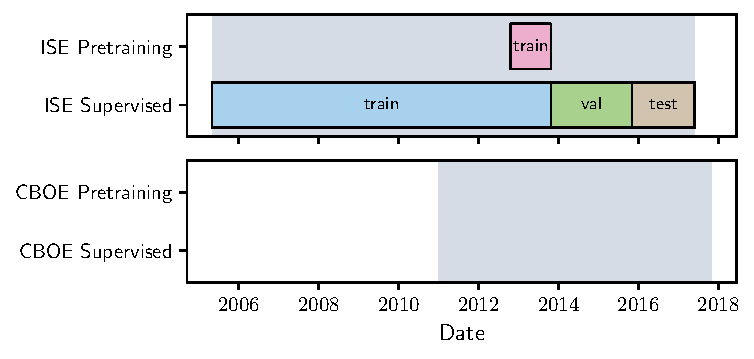
\includegraphics{train-test-split.pdf}
    \caption[Training Scheme on \glsentryshort{ISE} and \glsentryshort{CBOE} Sample]{Training scheme on \gls{ISE} and \gls{CBOE} sample. The train and validation set are split by time. Shaded area \mysquare{viz-gray} indicates the duration for which the dataset is available.}
    \label{fig:train-test-split}
\end{figure}

Overall, we use \gls{ISE} data from 2 May 2005 to 24 October 2013 to train and data between 25 October 2013 and 5 November 2015 to validate our models. The most recent trades until 31 May 2017 are used to assess the generalization error.

Models are pre-trained on unlabeled samples from the last six months of the training period. Given the significantly larger number of unlabeled customer trades, the pre-training period is reduced to facilitate training on the available computing resources.

We use the \gls{CBOE} sample past 5 November 2015 as a second test set, as visualized in \cref{fig:train-test-split}. Our evaluation approach is the most rigorous as it disallows any form of adaptation of the models, thereby ensuring a rigorous evaluation. Unlike transfer learning techniques such as parameter or model transfer, which expectedly improve model performance, we choose to forgo these techniques and demonstrate the effectiveness of our models without any transfer of knowledge. The start date ensures that leakage from the \gls{ISE} set is minimized.\footnote{The datasets contain features, such as the \gls{NBBO}, that are identical for both sets, assuming trades were executed at both exchanges simultaneously. Also, quotes can be identical between exchanges, if market makers quote at the \gls{NBBO}, which is common practice as documented in \textcite[][10]{securitiesandexchangecommissionReportConcerningExaminations2007}. Utilizing the full \gls{CBOE} sample could result in exaggerated performance estimates if the corresponding \gls{ISE} trade is used in training.}

Our train-test-split assumes that all subsets are drawn from the same distribution, so fitting a classifier on the training set and optimizing for the validation set provides good estimates for the test set. To validate this assumption, we use adversarial validation. Specifically, we re-label all training samples with $y=-1$ and all trades of the validation set with $y=1$, train a classifier on a random subset of the composed dataset, and predict class conformance. The performance is estimated using the \gls{MCC} of \textcite[][445]{matthewsComparisonPredictedObserved1975}, which ranges between $\left[-1, 1\right]$ and is insensitive to class imbalances.\footnote{Classes are imbalanced, due to the training set being three times the size of the validation set.} Assuming train and validation samples are sampled from the same distribution, the performance estimate is near a random guess, or $\operatorname{MCC} = 0$. For the mid-sized feature set, the \gls{MCC} is \num{0.364260805498287} suggesting training and validation sets are approximately similar. The next section discusses techniques used in training the classifiers.

\subsection{Training and Tuning}\label{sec:training-and-tuning}

The following section describes the experimental setup.\footnote{The authors acknowledge support by the federal state of Baden-Württemberg through \href{https://www.bwhpc.de/}{bwHPC}.} For reproducibility, the implementation and experiment tracking are publicly available.\footnote{Code is available at~\url{https://github.com/KarelZe/thesis}. Experiments are tracked at \url{https://wandb.ai/fbv/thesis}.}

\subsubsection{Training of Supervised
    Models}\label{sec:training-of-supervised-models}

Our implementation of \glspl{GBRT} is based on CatBoost \autocite[][5--6]{prokhorenkovaCatBoostUnbiasedBoosting2018} because of its efficient implementation on \glspl{GPU} and native support for categorical variables. However, as discussed in \cref{sec:gradient-boosting-procedure}, we expect the chosen library to have minimal impact on performance.

\begin{figure}[ht]
    \centering
    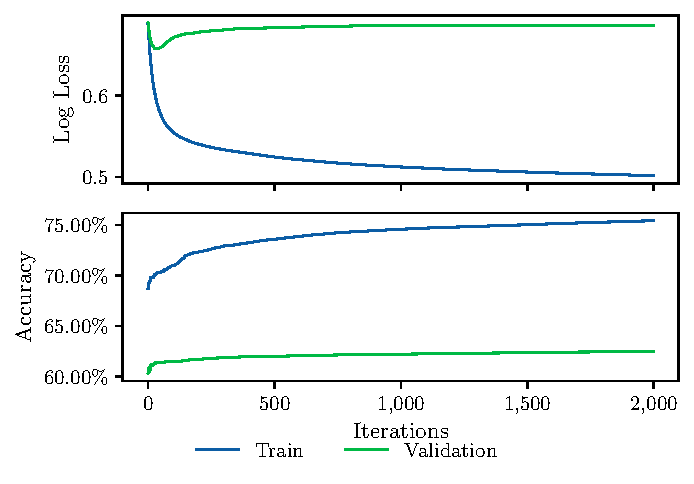
\includegraphics{gbm-train-val-loss-acc.pdf}
    \caption[Training and Validation Accuracy of Gradient Boosting]{Training and validation accuracy of \gls{GBRT} on \gls{ISE} sample. Metrics are estimated on the feature set classic. One iteration corresponds to an additional regression tree added to the ensemble. Loss is expected to decrease for more complex ensembles and accuracy to increase.}
    \label{fig:gbm-train-val-loss-acc}
\end{figure}

\cref{fig:gbm-train-val-loss-acc} displays the loss and accuracies of the default implementation on the \gls{ISE} training and validation set using classical features. The plots reveal several insights.

First, the model overfits the training data, as evident from the generalization gap between training and validation accuracies. To improve generalization performance, we apply regularization techniques.

Second, validation loss spikes for larger ensembles, while validation accuracy continues to improve. This discrepancy suggests that the predicted class's correctness improves, but the ensemble becomes less confident in the correctness of the prediction.

\begin{figure}[ht]
    \centering
    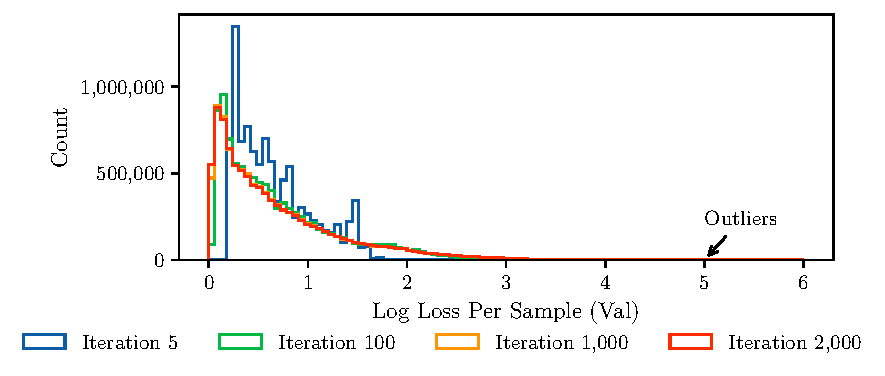
\includegraphics{gbm-loss-distribution.pdf}
    \caption[Sample-Wise Loss of Gradient Boosting]{Sample-wise log loss of \glsentryshort{GBRT} on \glsentryshort{ISE} sample as equi-width histogram. Loss is estimated on the classical feature set. In general, log loss improves for larger ensembles, as indicated by the increased number of samples accumulating around zero but few predictions contribute to the loss unproportionally causing the log loss to stagnate on average.}
    \label{fig:gbm-loss-distribution}
\end{figure}

This behavior can be explained by the log loss being unbound, where single incorrect predictions can cause the loss to explode. We verify this assumption by plotting the distribution of the sample-wise log loss in \cref{fig:gbm-loss-distribution}. As visible, loss per sample decreases for larger ensembles, at the same time few predictions contribute to the loss unproportionally, causing the average validation loss to stagnate.

\begin{figure}[ht]
    \centering
    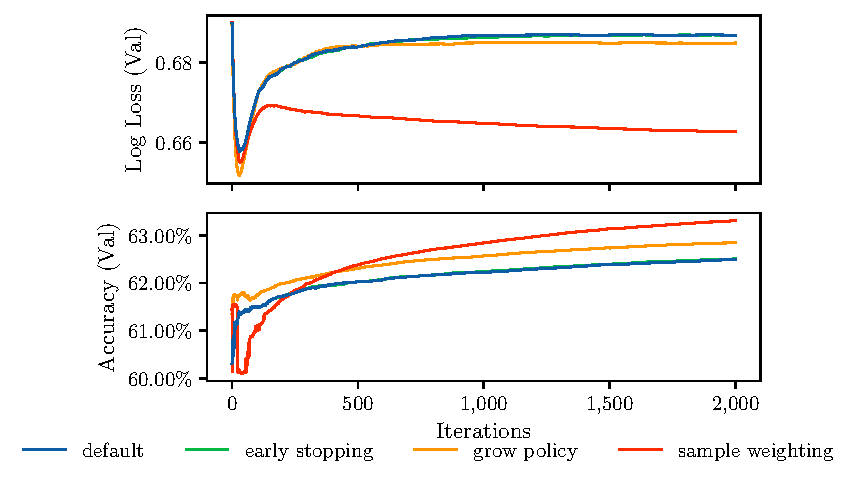
\includegraphics{gbm-optimisations-loss-acc.pdf}
    \caption[Training and Validation Accuracy of Gradient Boosting with Optimisations]{Training and validation accuracy of \gls{GBRT} on \gls{ISE} sample with optimizations. Metrics are estimated on the classical feature set. One iteration corresponds to an additional regression tree added to the ensemble. Loss is expected to decrease for more complex ensembles and accuracy to increase.}
    \label{fig:gbm-optimizations-loss-acc}
\end{figure}

We leverage several architectural changes to reduce the loss, further improve performance and mitigate overfitting in gradient boosting, as shown in \cref{fig:gbm-optimizations-loss-acc}, where the effects on validation accuracy and log loss over the default configuration are visualized. Following standard practice, e.g., \textcite[][]{tuningplaybookgithub}, all other parameters are kept at their default values, while a single parameter is varied to derive the plots. Although this approach ignores parameter interactions, it still can guide the optimal training configuration. We train on the \gls{ISE} training set with classical features and report metrics on the validation set.

\emph{Growth Strategy}

To improve performance, we switch to a leaf-wise growth strategy, following \textcite[][786]{chenXGBoostScalableTree2016}. By default, CatBoost grows oblivious regression trees, which are symmetric and grown level-wise. In this strategy, splits are performed on the same feature and split values across all nodes of a single level, which is computationally efficient but may compromise performance. In contrast, leaf-wise growth selects terminal nodes that provide the largest improvement in the loss, potentially leading to nodes within the same level being split with different features and values, resulting in a closer fit to the data. Leaf-wise growth also aligns with the intuition of split finding from \cref{sec:decision-tree}. This change improves validation accuracy by \SI{0.3461}{\percent} but has little effect on the loss.

\emph{Sample Weighting}

The work of \textcite[][35]{grauerOptionTradeClassification2022} suggests a strong temporal shift in the data, with the performance of classical trade classification rules deteriorating over time.  As a result, the predictability of features derived from these rules diminishes over time, and patterns learned from old observations become less relevant for predicting test samples. To address this, we introduce a sample weighting scheme that assigns higher weights to recent training samples and gradually decays weights over time, which we incorporate into the log loss. Validation and test samples are equally weighted. Sample weighting proves to be essential for achieving high validation performance, and it positively impacts the accuracy and confidence in the prediction mitigating the problem from above.

\emph{Border Count}

In regression trees of gradient boosting, the split finding is typically approximated with quantization, whereby all numeric features are first discretized into a fixed number of buckets through histogram building, and splits are evaluated at the border of the buckets \autocite[][3147]{keLightGBMHighlyEfficient2017}. To increase the number of split candidates, we raise the border count to \num{254}. Generally, this leads to increased accuracy at the cost of computational efficiency. Yet, in the experiment above, the improvements in validation loss and accuracy are minor compared to the previous modifications.

\emph{Early Stopping and Checkpointing}

To reduce overfitting, we monitor the training and validation accuracies when adding new trees to the ensemble and suspend training once validation accuracy decreases for \num{100} iterations. The ensemble is then cut back to achieve the highest validation accuracy. In the experiment above, early stopping does not apply, as validation accuracy continues to improve for larger ensembles. We employ additional measures to address overfitting but treat them as a tunable hyperparameter, with further details provided in \cref{sec:hyperparameter-tuning}. We incorporate all ideas into our large-scale studies.

\textbf{FT-Transformer}

We rely on the FT-Transformer of \textcite[][18935--18936]{gorishniyRevisitingDeepLearning2021} as our second model. The training of Transformers has been found non-trivial and requires a carefully designed training setup of model, optimizer, and learning rate schedule \autocite[][5747]{liuUnderstandingDifficultyTraining2020}. We investigate minor modifications to the default FT-Transformer to stabilize training and improve overall performance. The default FT-Transformer is trained for 10 epochs on the \gls{ISE} dataset with classical features and loss and accuracy are visualized in \cref{fig:fttransformer-optimizations-loss-acc}.\footnote{Default configuration documented in \textcite[][sup.]{gorishniyRevisitingDeepLearning2021}.}

The convergence behavior of our model is similar to that of gradient boosting. Equally, a significant generalization gap exists between the training and validation loss. The training loss decreases sharply, while the validation loss spuriously improves over its initial estimate. Despite this, validation accuracy improves throughout the entire training cycle. We reason that the network learns to correctly classify trades, indicated by the improved accuracy, but only attains low-confident correct predictions or confident but erroneous predictions which both contribute to a large validation loss.

\begin{figure}[!ht]
    \centering
    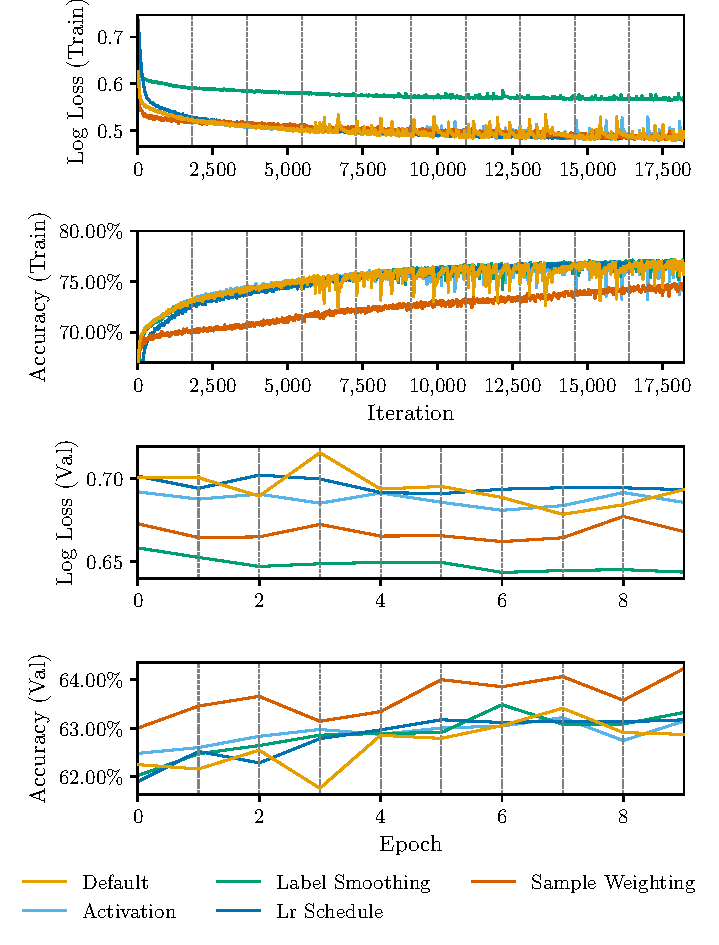
\includegraphics{fttransformer-optimisations-loss-acc.pdf}
    \caption[Training and Validation Accuracy of FT-Transformer with Optimisations]{Training and validation accuracy of FT-Transformer on \gls{ISE} sample with optimizations. Metrics are estimated on the classical feature set. One iteration corresponds to one gradient update. The end of each epoch is marked with a dashed bar. Loss is expected to decrease throughout training and accuracy to increase.}
    \label{fig:fttransformer-optimizations-loss-acc}
\end{figure}

\textbf{Solutions For FT-Transformer}

\emph{Activation Function}

Motivated by previous research, we experiment with replacing the $\operatorname{ReLU}$ activation with the $\operatorname{GELU}$ activation function \autocite[][2]{hendrycksGaussianErrorLinear2020} in the classification head and the gated variant $\operatorname{ReGLU}$ with the gated variant $\operatorname{GEGLU}$ \autocite[][2]{shazeerGLUVariantsImprove2020} in the \gls{FFN}. As visualized in \cref{fig:fttransformer-optimizations-loss-acc}, no advantage in terms of validation accuracy or loss is evident.

\emph{Sample Weighting}

We apply the concept of sample weighting from \gls{GBRT} to Transformers. Specifically, we scale the contribution of individual training samples to the loss using a sample weight, which penalizes the model for misclassifying recent observations. This method is crucial for achieving low validation loss and high validation accuracies, as visible in \cref{fig:fttransformer-optimizations-loss-acc}. The significantly lower training accuracy implies, that patterns from latter observations do not universally transfer to previous observations. It remains unclear what is causing the data drift within the training set.

\clearpage

\emph{Label Smoothing}

A major problem in classification with neural networks is, that the network becomes overconfident in predicting training samples but performs poorly on unseen data. In \cref{fig:fttransformer-optimizations-loss-acc} the effect is evident, as the increased confidence in the prediction on the training set does not transfer to the validation set. To regularize the network, we experiment with label smoothing \autocite[][2823]{szegedyRethinkingInceptionArchitecture2016} by training on soft labels with an uncertainty constant of $\epsilon$. Instead of assigning hard class probabilities of 0 or 1, we assume that true labels in the training set are correct with $1-\epsilon$ probability and incorrect otherwise. For $\epsilon=\num{0.1}$, a trade with the true label $-1$ is assumed to be \SI{90}{\percent} seller-initiated and \SI{10}{\percent} buyer-initiated. While we observe that label smoothing improves the validation loss and reduces the generalization gap, we find that it has a negligible effect on validation accuracy and therefore abandon the approach.

\emph{Learning Rate Schedule}

When training Transformers, the learning rate is often adjusted throughout the training process. \textcite[][6007]{vaswaniAttentionAllYou2017} use a learning rate warm-up period, whereby the learning rate is linearly increased in the early stages of training, followed by decay using an inverse square root learning rate schedule. The warm-up phase is thought to stabilize gradients as weight updates are considerably smaller. According to \cref{sec:residual-connections-layer-norm}, learning rate warm-up is crucial for training post-norm Transformers, but optional for pre-norm Transformers like the FT-Transformer. Nevertheless, we experiment with the effect of learning rate warm-up in our setting and combine a linear warm-up for two epochs with subsequent cosine decay, as visualized in \cref{fig:lr-lin-warmup-cosine-decay}.

\begin{figure}[!ht]
    \centering
    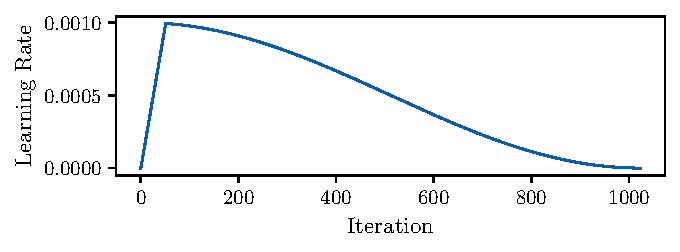
\includegraphics{lr-lin-warmup-cosine-decay.pdf}
    \caption[Linear Learning Rate Warm-Up With Cosine Decay]{Linear learning rate warm-up with cosine decay. Warm-up is performed for the first \SI{5}{\percent} of iterations. In the example, the maximum learning rate is \num{1e-3}.}
    \label{fig:lr-lin-warmup-cosine-decay}
\end{figure}

The scheduled learning rate smooths the training loss and accuracy estimates, as evident in \cref{fig:fttransformer-optimizations-loss-acc}. Therefore, we adopt a training setup with a learning rate schedule, despite the negative effects on training time. The learning rate itself is tuned as part of \cref{sec:hyperparameter-tuning}.

\emph{Batch Size}

% 20 epochs (\num{36460} / \num{145840} iterations) 
We use a fixed batch size of \num{8192} samples for the feature set classic/size and \num{2048} for the feature set option, which is the largest possible size on our \gls{GPU}. Training is performed for \num{20} epochs at maximum. All samples within the training and validation set are shuffled randomly to promote convergence. Although a smaller batch size could enhance the generalization capabilities of the model, as found in \textcite[][3]{keskarLargeBatchTrainingDeep2017}, we train on the largest number of trades per iteration, to optimize throughput. Additional regularization is added to the model, but treated as a tunable hyperparameter.

\emph{Early Stopping and Checkpointing}

Similar to the \gls{GBRT}, we halt training prematurely based on a consecutive decrease in validation accuracy. We set the patience to \num{10} epochs and restore the best model in terms of validation accuracy from the checkpoint. Checkpoints are saved at the end of each epoch. In the experiment above, early stopping does not apply.

\emph{Optimizer}

In line with \textcite[][18937]{gorishniyRevisitingDeepLearning2021}, we train the models using the AdamW optimizer \autocite[][2--3]{loshchilovDecoupledWeightDecay2019} with the standard hyperparameters.\footnote{Parameters $\beta_{1}=0.9, \beta_{2}=0.999$, and $\epsilon = \num{1e-8}$.} The weight decay coefficient in AdamW determining the degree of regularization is tuned in \cref{sec:hyperparameter-tuning}. Weight decay is selectively applied and excludes embeddings, normalization layers, and biases.

In summary, we extend the training setup of \textcite[][18937]{gorishniyRevisitingDeepLearning2021} with a sample weighting scheme and learning rate schedule aimed at boosting performance and training stability.

\vskip 1.3in

\textbf{Solutions For Classical Rules}

Classical trade classification rules serve as a benchmark in our work. We implement them as a classifier that combines arbitrary trade classification rules through stacking, as covered in \cref{sec:semi-supervised-approaches}.

In cases where classification is not feasible due to missing data or the rules' definition itself, we resort to a random classification, which achieves an average accuracy of \SI{50}{\percent}. The approach is adopted from \textcite[][887]{savickasInferringDirectionOption2003}.

\subsubsection{Training of Semi-supervised
    Models}\label{sec:training-of-semi-supervised-models}

This section discusses the extensions necessary to train the semi-supervised variants of \glspl{GBRT} and the FT-Transformer.

\textbf{Gradient Boosting With Self-Training}

To incorporate unlabeled trades into the training procedure, we combine gradient boosting with a self-training classifier, as derived in \cref{sec:extensions-to-gradient-boosted-trees}. We repeat self-training for 2 iterations and require the predicted class probability to exceed $\tau=0.9$. As the entire ensemble is rebuilt three times, the low number of iterations and high confidence threshold, strike a balance between computational requirements and the need for high-quality predictions. The base classifier is otherwise identical to supervised gradient boosting from \cref{sec:training-of-supervised-models}.

\textbf{FT-Transformer With Pre-Training}

The FT-Transformer is trained in two stages. First, we train for \num{20} epochs on unlabeled \gls{ISE} trades using the \gls{RTD} head, followed by \num{20} epochs of fine-tuning on labeled \gls{ISE} training data with the binary classification head.

During pre-training and fine-tuning, early stopping is applied based on the value of the objective on the validation set, using patience of \num{10}. This particular setup is adopted from \textcite[][15]{rubachevRevisitingPretrainingObjectives2022} for being compute-efficient and offering competitive performance on tabular datasets. The hidden dimension of the classification head is set to \num{512}. Based on \textcite[][3]{clarkElectraPretrainingText2020} \SI{15}{\percent} of all tokens are replaced.

Since the unlabeled sample includes various types of trades that may not be comparable to the labeled sample, we update all layers during fine-tuning. Empirically, fine-tuning the entire model is among the most successful methods, as results from \textcite[][104--105]{raeScalingLanguageModels2022} for Transformers in general and results from \textcite[][39]{merchantWhatHappensBERT2020} specific for \gls{BERT}-like architectures document. Yet, updating all layers is the most resource-intensive.

Following \textcite[][4]{rubachevRevisitingPretrainingObjectives2022}, the learning rate and weight decay are shared between the pre-training and fine-tuning stages. All other hyperparameters related to the model are identical.

\subsubsection{Hyperparameter Tuning}\label{sec:hyperparameter-tuning}

All of our machine-learning models feature a set of tunable hyperparameters. The results of previous studies, exemplary the one of \textcite[][511]{grinsztajnWhyTreebasedModels2022}, emphasize the need for tuning routines, as the test performance of the FT-Transformer and \glspl{GBRT} largely fluctuates with the hyperparameter configuration. Classical rules have no hyperparameters per se, but the best hybrid rules can be attained through hyperparameter search.
For a fair comparison, we employ an exhaustive hyperparameter search, to find a suitable hyperparameter configuration for each of our models.

\textbf{Bayesian Search}

We run a novel Bayesian search to suggest and tune the hyperparameters automatically. In Bayesian search, a prior belief for all possible objective functions is formulated from the parameter intervals, which is then gradually refined by updating the Bayesian posterior with data from previous trials thereby approximating the likely objective function \autocite[][149]{shahriariTakingHumanOut2016}. Compared to brute-force approaches, such as grid search, unpromising search regions are omitted, resulting in more promising trials.

While different algorithmic implementations exist for Bayesian optimization, we choose the \emph{Optuna} library \autocite[][2623--2631]{akibaOptunaNextgenerationHyperparameter2019}, which implements the tree parzen estimator algorithm and is capable of handling both continuous and categorical hyperparameters.\footnote{Implementation of the tree-parzen estimator searches the first 10 trials randomly before the completed trials affect the sampling.} We maximize the accuracy of the validation set, which is also our decisive metric for evaluation (cp. \cref{sec:evaluation-metric}), and run $\num{50}$ trials per feature set for the \gls{GBRT} and $\num{10}$ trials for the FT-Transformer. The best combination of each is tested out-of-sample in \cref{sec:results}.

\textbf{Gradient Boosting}

Our search space is reported in \cref{tab:hyperparameter-space-gbm}, which is loosely aligned with \textcite[][sup.]{gorishniyRevisitingDeepLearning2021}.

\begin{table}[!h]
    \centering
    \sisetup{table-number-alignment=left}
    \caption[Hyperparameter Search Space of Gradient Boosting]{Hyperparameter search space of gradient boosting.}
    \label{tab:hyperparameter-space-gbm}
    \begin{tabular}{@{}ll@{}}
        \toprule
        Hyperparameter               & Distribution                                  \\ \midrule
        Depth                        & $\operatorname{UniformInt}[1,12]$             \\
        Learning rate $\eta$         & $\operatorname{LogUniform}[0.001, 0.125]$     \\
        $\ell_2$ Leaf regularization & $\operatorname{UniformInt}[2, 30]$            \\
        Random strength              & $\operatorname{LogUniform}[\num{1e-9}, 10.0]$ \\
        Bagging temperature          & $\operatorname{Uniform}[0.0, 1.0]$            \\ \bottomrule
    \end{tabular}
\end{table}

As documented, we tune five hyperparameters for gradient boosting. The first is the depth, which determines the number of levels in each tree. Other than \textcite[][sup.]{gorishniyRevisitingDeepLearning2021}, we increase the upper bound to twelve to allow for more complex ensemble members. Acknowledging the research of \textcite[][1203]{friedmanGreedyFunctionApproximation2001} that the learning rate \eta~and the size of the ensemble have a strong interdependence, we only tune the learning rate and stop extending the ensemble based on the early stopping criterion. Random strength, bagging temperature, and $\ell_2$ leaf regularization are measures to counter overfitting. Specifically, random strength controls the degree of Gaussian noise added to the scores of split candidates to introduce randomness in the selected splits. In a similar vein, the algorithm introduces randomness on the sample level through Bayesian bootstrap \autocite[][130--131]{rubinBayesianBootstrap1981}. The hyperparameter controls the distribution used for sampling, and implicitly the aggressiveness of bagging. Finally, $\ell_2$ leaf regularization adds a penalty term to the terminal leaf's estimates. The hyperparameter controls the degree of regularization.

\begin{figure}[!h]
    \subfloat[Hyperparameter Search Space of \gls{GBRT} With Feature Set Classic\label{fig:ise-gbm-hyperparam-classical}]{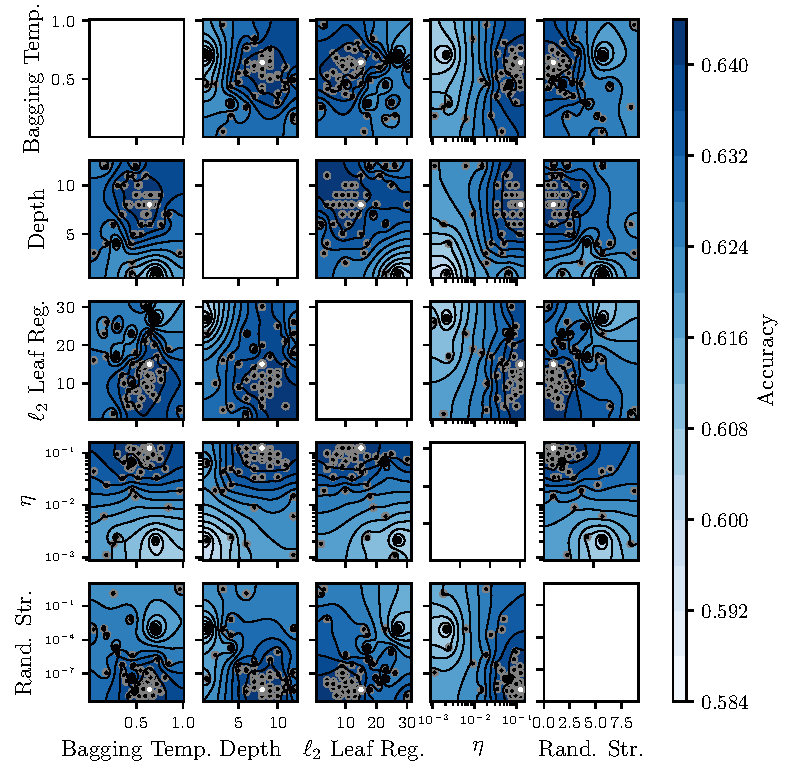
\includegraphics[width=0.6\textwidth]{1gzk7msy-hyperparam-search-space.pdf}}
    \vfill
    \subfloat[Hyperparameter Search Space of \gls{GBRT} With Feature Set Size\label{fig:ise-gbm-hyperparam-classical-size}]{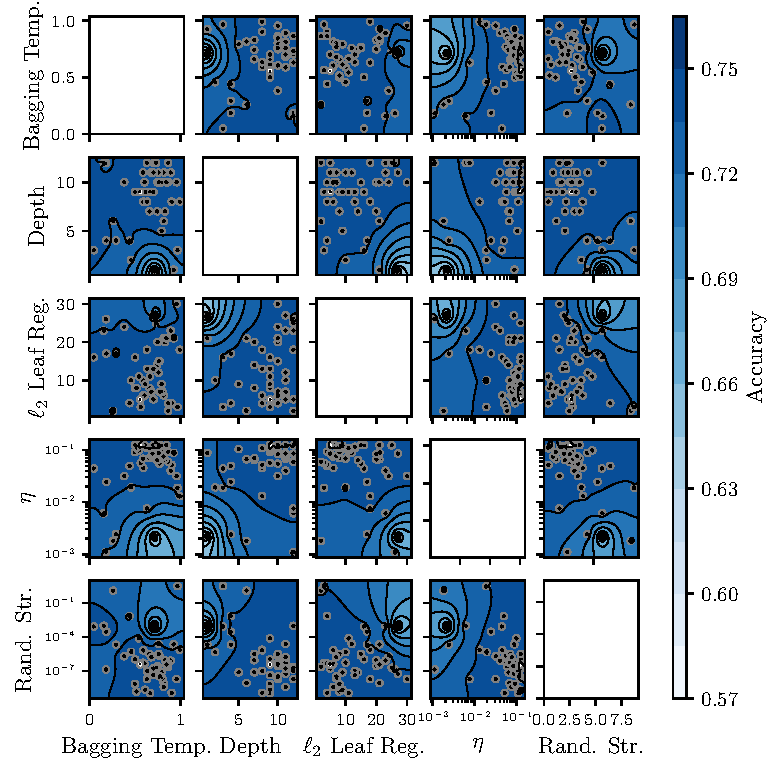
\includegraphics[width=0.6\textwidth]{3vntumoi-hyperparam-search-space.pdf}}
    \caption[Hyperparameter Search Space of Gradient Boosting]{Hyperparameter Search Space of \gls{GBRT} on \gls{ISE} Validation Set}
    \label{fig:ise-gbm-hyperparam}
\end{figure}
\clearpage
\begin{figure}[!ht]
    \ContinuedFloat
    \subfloat[Hyperparameter Search Space of \gls{GBRT} With Feature Set Option\label{fig:ise-gbm-hyperparam-ml}]{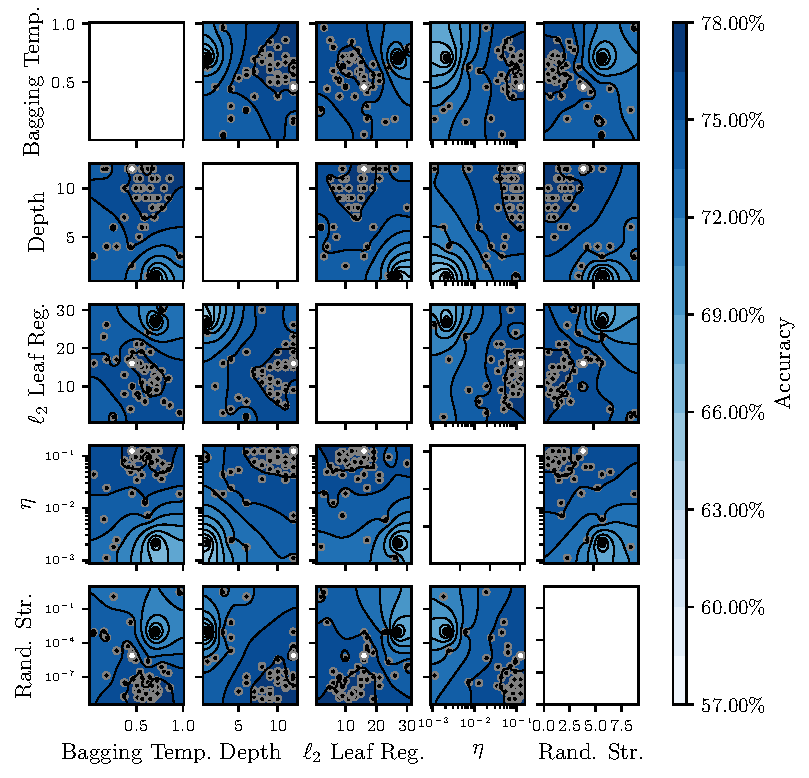
\includegraphics[width=0.6\textwidth]{2t5zo50f-hyperparam-search-space.pdf}}
\end{figure}

\cref{fig:ise-gbm-hyperparam-classical} visualizes the hyperparameter search space of the \gls{GBRT} on the \gls{ISE} dataset with classical features, from which we can derive several observations. First, hyperparameter tuning has a significant impact on the prediction, as the validation accuracy varies between \SI{58.429}{\percent} and \SI{64.378}{\percent} for different trials. Second, the best hyperparameter combination, marked with \bestcircle, lies off-the-borders surrounded by other promising trials, indicated by the contours, from which we can conclude, that the found solution is a stable and reasonable choice for further analysis.

In \cref{fig:ise-gbm-hyperparam-classical-size} we repeat the analysis for \glspl{GBRT} trained on size features. The loss surface is smooth with large connected regions. As the best solution achieving \SI{75.03504680858162}{\percent} accuracy lies within a splayed region of dense sampling, it is a good choice for further analysis. Consistent with the loss surface of \cref{fig:ise-gbm-hyperparam-classical}, the trees are grown to the maximum depth and a high learning rate, indicating the need for complex ensemble members highly corrective to previous predictions. Part of this could be due to the low signal-to-noise ratio in financial data.

The loss surface of the \gls{GBRT} trained on the feature set including option features is the least fragmented. While the validation accuracy of the best combinations improves significantly to \SI{76.99459643967347}{\percent}, worst trials even underperform these of smaller feature sets. We note, more data does not per se improve the model and that models require a thoughtful tuning procedure. Our conclusion contradicts the one of \textcite[][14]{ronenMachineLearningTrade2022}, who find no advantage in tuning tree-based ensembles for trade classification. Results are tabulated in \cref{tab:solutions-gbm}.

\begin{table}[!h]
    \centering
    \sisetup{table-format=3.2,table-alignment-mode = none, table-number-alignment=left, table-text-alignment = left}
    \caption[Search Solutions of Gradient Boosting]{Search solutions of gradient boosting. The three right columns document the best combination in terms of validation accuracy per feature set. We perform \num{50} trials.}
    \label{tab:solutions-gbm}
    \begin{tabular}{@{}llSSS@{}}
        \toprule
        Hyperparameter               & Distribution                                  & {\glsentryshort{FS} Classic} & {\glsentryshort{FS} Size} & {\glsentryshort{FS} Option} \\ \midrule
        Depth                        & $\operatorname{UniformInt}[1,12]$             & 8                            & 9                         & 12                          \\
        Learning rate $\eta$         & $\operatorname{LogUniform}[0.001, 0.125]$     & 0.12484221864046671          & 0.12347889459796775       & 0.12471458170177774         \\
        $\ell_2$ Leaf regularization & $\operatorname{UniformInt}[2, 30]$            & 15                           & 5                         & 16                          \\
        Random strength              & $\operatorname{LogUniform}[\num{1e-9}, 10.0]$ & \num{4e-9}                   & \num{4e-7}                & \num{8e-6}                  \\
        Bagging temperature          & $\operatorname{Uniform}[0.0, 1.0]$            & 0.6419530220498153           & 0.5574912093427532        & 0.45578836944233            \\ \midrule
        Validation Accuracy in \%    &                                               & 64.37816236230594            & 75.03504680858162         & 76.99459643967347           \\ \bottomrule
    \end{tabular}
\end{table}

\textbf{Gradient Boosting With Self-Training}

The search space for the semi-supervised variant is identical to the supervised gradient boosting. To conserve space, we only report the tabulated results in \cref{tab:solutions-GBRT-self-training}.\footnote{Visualizations of the hyperparameter search space are available online. See \url{https://wandb.ai/fbv/thesis/runs/37lymmzc} for \gls{FS} classic, \url{https://wandb.ai/fbv/thesis/runs/324v3uv5} for \gls{FS} size, and \url{https://wandb.ai/fbv/thesis/runs/t55nd8r0} for \gls{FS} option.}

\begin{table}[!h]
    \centering
    \sisetup{table-format=3.2,table-alignment-mode = none, table-number-alignment=left, table-text-alignment = left}
    \caption[Search Solutions of Gradient Boosting With Self-Training]{Search solutions of gradient boosting with self-training. The three right columns document the best combination in terms of validation accuracy per feature set. We perform \num{50} trials. Arrows indicate the change compared to the supervised variant.}
    \label{tab:solutions-GBRT-self-training}
    \begin{tabular}{@{}llSSS@{}}
        \toprule
        Hyperparameter               & Distribution                                  & {\glsentryshort{FS} Classic}                                & {\glsentryshort{FS} Size}                                   & {\glsentryshort{FS} Option}                                 \\ \midrule
        Depth                        & $\operatorname{UniformInt}[1,12]$             & 9                                                           & 10                                                          & 9                                                           \\
        Learning rate $\eta$         & $\operatorname{LogUniform}[0.001, 0.125]$     & 0.12337960608926582                                         & 0.1248422186404667                                          & 0.12347504812996231                                         \\
        $\ell_2$ Leaf regularization & $\operatorname{UniformInt}[2, 30]$            & 12                                                          & 9                                                           & 13                                                          \\
        Random strength              & $\operatorname{LogUniform}[\num{1e-9}, 10.0]$ & \num{2e-8}                                                  & \num{5e-8}                                                  & \num{5e-8}                                                  \\
        Bagging temperature          & $\operatorname{Uniform}[0.0, 1.0]$            & 0.34010535578784745                                         & 0.5214954412829511                                          & 0.4666577105566224                                          \\ \midrule
        Validation Accuracy in \%    &                                               & {$\textcolor{viz-red}{\downarrow} \num{64.29671279599335}$} & {$\textcolor{viz-red}{\downarrow} \num{74.83010065958079}$} & {$\textcolor{viz-red}{\downarrow} \num{76.41433947686962}$} \\ \bottomrule
    \end{tabular}
\end{table}

Matching the supervised results, semi-supervised ensembles exhaust the maximum tree depth and combine trees with a coarse learning rate. By parameter importance, both are most influential on the final result. Again, this is an indication that the trade data is not easily separable, requiring multiple features and splits. The found hyperparameters for $\ell_2$ leaf regularization, random strength, and bagging are balanced. Overall, the best validation accuracies are slightly inferior to the supervised variant.


\textbf{FT-Transformer}

The search space for the FT-Transformer is identical to \textcite[][sup.]{gorishniyRevisitingDeepLearning2021} (variant (b)) with minor deviations and reported in \cref{tab:hyperparameter-space-2}.

\begin{table}[!h]
    \centering
    \sisetup{table-format=3.2,table-alignment-mode = none, table-number-alignment=left, table-text-alignment = left}
    \caption[Hyperparameter Search Space of FT-Transformer]{Hyperparameter search space of FT-Transformer.}
    \label{tab:hyperparameter-space-2}
    \begin{tabular}{@{}ll@{}}
        \toprule
        Hyperparameter         & Distribution                                        \\ \midrule
        Layers $L$             & $\operatorname{UniformInt}[1,6]$                    \\
        Attention dropout      & $\operatorname{Uniform}[0, 0.5]$                    \\
        \gls{FFN} dropout      & $\operatorname{Uniform}[0, 0.5]$                    \\
        Weight decay $\lambda$ & $\operatorname{LogUniform}[\num{3e-5}, \num{3e-4}]$ \\
        Learning rate $\eta$   & $\operatorname{LogUniform}[\num{1e-6}, \num{1e-3}]$ \\ \bottomrule
    \end{tabular}
\end{table}

We vary the layer count and the embedding dimension, which directly affect the capacity of the network. Layers refer to the number of Transformer blocks in the encoder stack. The dimension of numerical and continuous embeddings $d_e$ is at \num{256} at maximum, which is half the dimension used in the author's work. We make this sacrifice, due to being computation-bound by the size of the dataset. Dropout in the attention module and the \gls{FFN} is used to prevent overfitting the training data. As discussed in \cref{sec:training-of-supervised-models}, we treat the weight decay term in the weight update rule of the AdamW optimizer as a hyperparameter, with larger values for \lambda~enforcing a stronger shrinkage of weights and thereby reducing overfitting.

Due to the pseudo-random sampling during the first trials of Bayesian search combined with the reduced number of trials for the Transformer studies, the tested hyperparameter combinations are identical for all feature sets, as visible in \cref{fig:ise-transformer-hyperparam}.

\begin{figure}[!h]
    \subfloat[Hyperparameter Search Space of FT-Transformer With Feature Set Classic\label{fig:ise-transformer-hyperparam-classical}]{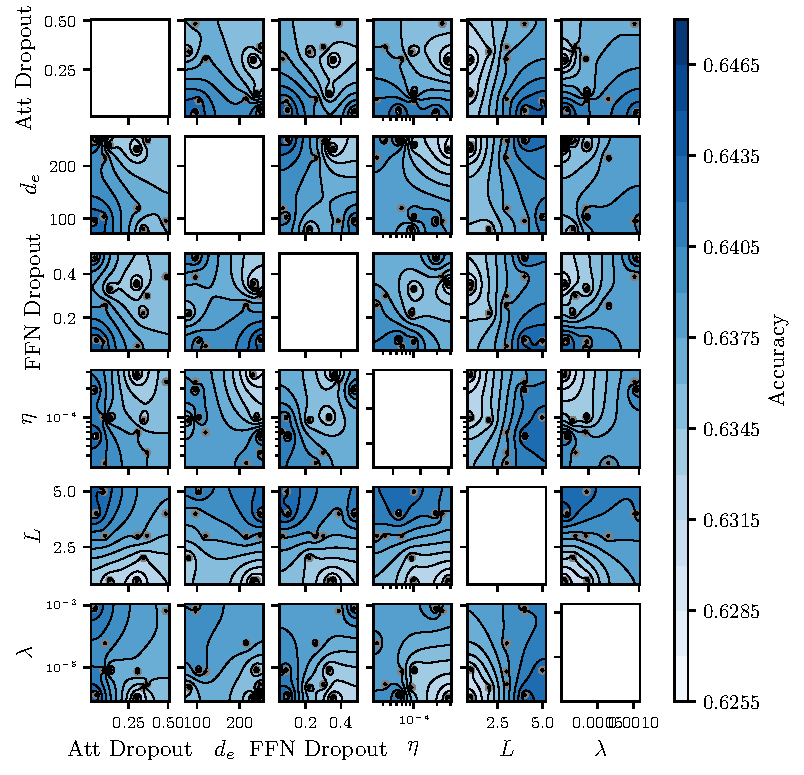
\includegraphics[width=0.6\linewidth]{3jpe46s1-hyperparam-search-space.pdf}}
    \vfill
    \subfloat[Hyperparameter Search Space of FT-Transformer With Feature Set Size\label{fig:ise-transformer-hyperparam-classical-size}]{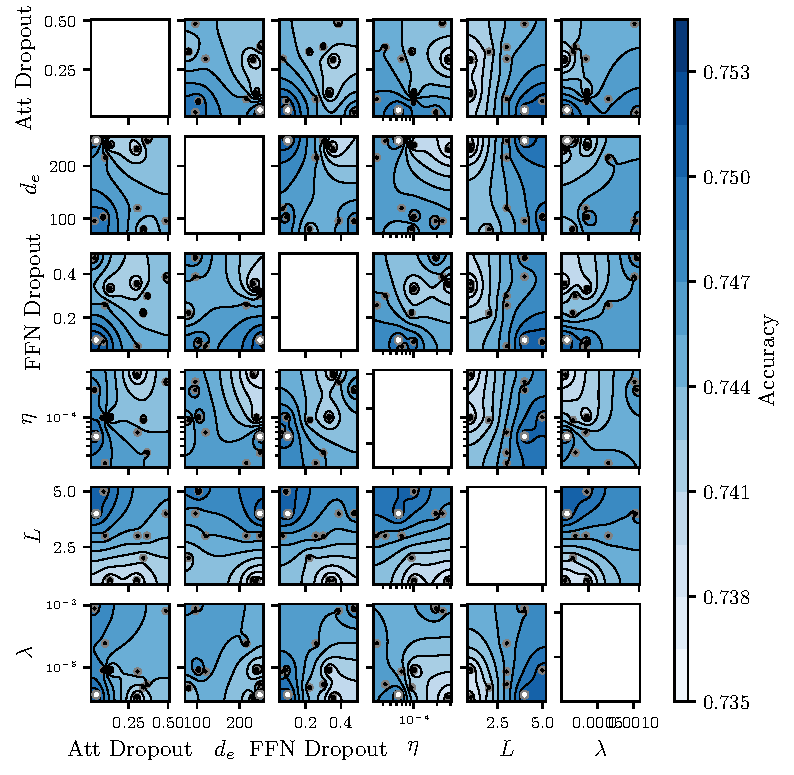
\includegraphics[width=0.6\linewidth]{1qx3ul4j-hyperparam-search-space.pdf}}
    \caption[Hyperparameter Search Space of FT-Transformer]{Hyperparameter Search Space of FT-Transformer on \gls{ISE} Validation Set}
    \label{fig:ise-transformer-hyperparam}
\end{figure}
\clearpage
\begin{figure}[!ht]
    \ContinuedFloat
    \subfloat[Hyperparameter Search Space of \gls{GBRT} With Feature Set Option\label{fig:ise-transformer-hyperparam-ml}]{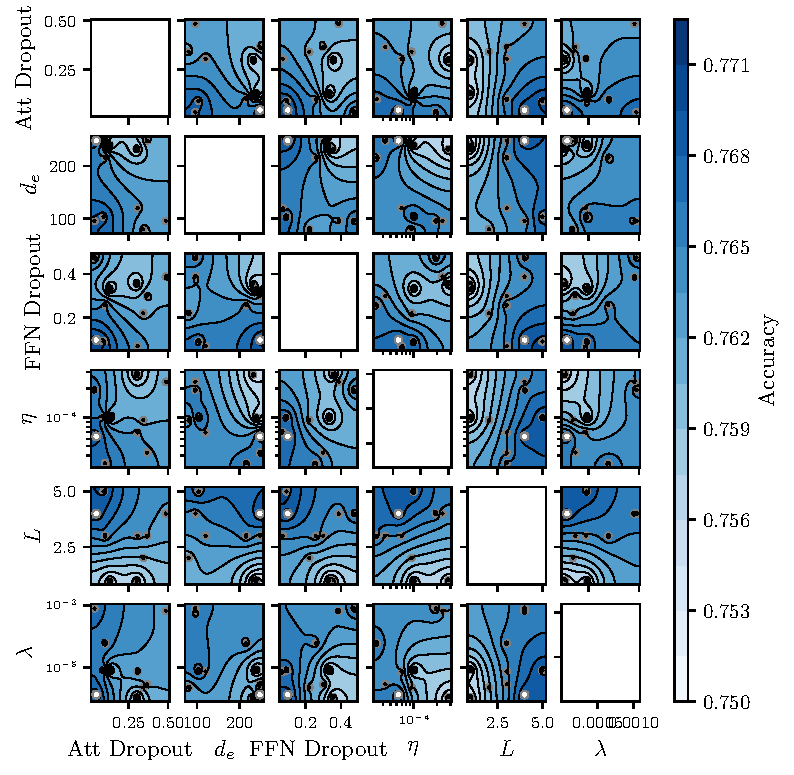
\includegraphics[width=0.6\linewidth]{2h81aiow-hyperparam-search-space.pdf}}
\end{figure}

With the smaller number of trials, the search space is less densely populated. Despite the decreased coverage, for the searched combinations the impact of hyperparameter tuning is less pronounced than for the \gls{GBRT}. As such, accuracies for \cref{fig:ise-transformer-hyperparam-classical} fluctuate between \SI{62.55}{\percent} and \SI{64.65}{\percent}. This translates to other feature sets. Unaffected, the validation accuracies are higher than for gradient boosting.

The best combination is identical for all feature sets. The embedding dimension is at \num{248}, which is almost maxed out and the model uses four Transformer blocks. Thus, it has a medium capacity with \num{1985649} to \num{4252369} parameters, depending on the feature set. From all hyperparameters, the number of layers is most impactful on the final accuracy. While the use of dropout and weight decay for regularization is minimal and marginally affects the validation performance. The large token dimensionality and mid-layer count could be an indication, that few attention heads are enough to extract patterns, but the learned patterns are relatively complex. The search results are compiled in \cref{tab:solutions-transformer}.

\begin{table}[!h]
    \centering
    \sisetup{table-format=3.2,table-alignment-mode = none, table-number-alignment=left, table-text-alignment = left}
    \caption[Search Solutions of FT-Transformer]{Search solutions of FT-Transformer. The three right columns document the best combination in terms of validation accuracy per feature set. We perform \num{10} trials. A discussion of these results is provided below.}
    \label{tab:solutions-transformer}
    \begin{tabular}{@{}llSSS@{}}
        \toprule
        Hyperparameter                       & Distribution                                        & {\glsentryshort{FS} Classic} & {\glsentryshort{FS} Size} & {\glsentryshort{FS} Option} \\ \midrule
        Layers $L$                           & $\operatorname{UniformInt}[1,6]$                    & 4                            & 4                         & 4                           \\
        Embedding dimension $d_{\mathrm{e}}$ & $\operatorname{UniformInt}[64, 256]$                & 248                          & 248                       & 248                         \\
        Attention dropout                    & $\operatorname{Uniform}[0, 0.5]$                    & 0.04424625102595975          & 0.04424625102595975       & 0.04424625102595975         \\
        \gls{FFN} dropout                    & $\operatorname{Uniform}[0, 0.5]$                    & 0.0979914312095726           & 0.0979914312095726        & 0.0979914312095726          \\
        Weight decay $\lambda$               & $\operatorname{LogUniform}[\num{3e-5}, \num{3e-4}]$ & \num{1e-6}                   & \num{1e-6}                & \num{1e-6}                  \\
        Learning rate $\eta$                 & $\operatorname{LogUniform}[\num{1e-6}, \num{1e-3}]$ & \num{6e-5}                   & \num{6e-5}                & \num{6e-5}                  \\ \midrule
        Validation Accuracy in \%            &                                                     & 64.69                        & 75.42                     & 77.17                       \\ \bottomrule
    \end{tabular}
\end{table}

\vskip 1.3in

\textbf{FT-Transformer With Pre-Training}

The hyperparameter search space for Transformers with a pre-training objective is identical to that shown in \cref{tab:hyperparameter-space-2}. As evident from \cref{tab:solutions-transformer-pretraining}, the found solutions are identical to these of the FT-Transformer without pre-training and identical for all three feature sets. During pre-training, we can detect if a token is replaced with \SI{94.06319856643677}{\percent} to \SI{95.89540958404541}{\percent} accuracy.\footnote{Na\"ive prediction yields \SI{85}{\percent} accuracy given the chosen replacement rate.}

\begin{figure}[!h]
    \centering
    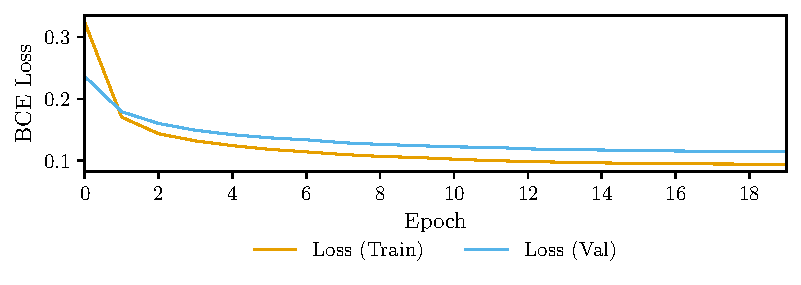
\includegraphics{transformer_ise_pretrain_classical.pdf}
    \caption[Pre-Training Loss of FT-Transformer]{Pre-training loss on \gls{ISE} sample with \gls{FS} classic. Training is performed for 20 epochs. Loss is the mean over all batches per epoch.}
    \label{fig:fttransformer-pretrain-loss}
\end{figure}

Pre-training performance is however bound by the available computing budget. As evident from \cref{fig:fttransformer-pretrain-loss}, the models have not fully converged until the end of pre-training, as the loss on the train- and validation set steadily improves.

Validation accuracy after fine-tuning improves for all models over Transformers without pre-training. As the search space is identically sampled for both variants we can directly attribute the improvements of \SI{0.28}{\percent} to \SI{0.72}{\percent} in validation accuracy to pre-training on unlabeled trades.\footnote{Visualizations of the hyperparameter search spaces are available online. See \url{https://wandb.ai/fbv/thesis/runs/12isqh2m} for \gls{FS} classic, for \url{https://wandb.ai/fbv/thesis/runs/2hv1nayy} for \gls{FS} size, and \url{https://wandb.ai/fbv/thesis/runs/3jbqpp4r} for \gls{FS} option for details.}


\begin{table}[!h]
    \centering
    \sisetup{table-format=3.2,table-alignment-mode = none, table-number-alignment=left, table-text-alignment = left}
    \caption[Search Solutions of FT-Transformer With Pre-Training]{Search solutions of FT-Transformer with pre-training. The three right columns document the best combination in terms of validation accuracy per feature set. We perform \num{10} trials. Arrows indicate the change compared to the supervised variant.}
    \label{tab:solutions-transformer-pretraining}
    \begin{tabular}{@{}llSSS@{}}
        \toprule
        Hyperparameter                       & Distribution                                        & {\glsentryshort{FS} Classic}                               & {\glsentryshort{FS} Size}                                   & {\glsentryshort{FS} Option}                       \\ \midrule
        Layers $L$                           & $\operatorname{UniformInt}[1,6]$                    & 4                                                          & 4                                                           & 4                                                 \\
        Embedding dimension $d_{\mathrm{e}}$ & $\operatorname{UniformInt}[64, 256]$                & 248                                                        & 248                                                         & 248                                               \\
        Attention dropout                    & $\operatorname{Uniform}[0, 0.5]$                    & 0.04424625102595975                                        & 0.04424625102595975                                         & 0.04424625102595975                               \\
        \gls{FFN} dropout                    & $\operatorname{Uniform}[0, 0.5]$                    & 0.0979914312095726                                         & 0.0979914312095726                                          & 0.0979914312095726                                \\
        Learning rate $\eta$                 & $\operatorname{LogUniform}[\num{3e-5}, \num{3e-4}]$ & \num{1e-6}                                                 & \num{1e-6}                                                  & \num{1e-6}                                        \\
        Weight decay $\lambda$               & $\operatorname{LogUniform}[\num{1e-6}, \num{1e-3}]$ & \num{6e-5}                                                 & \num{6e-5}                                                  & \num{6e-5}                                        \\ \midrule
        Validation Accuracy \%               & Pre-Train                                           & {\num{95.89540958404541}}                                  & {\num{95.64009308815002}}                                   & {\num{94.06319856643677}}                         \\
                                             & Fine-Tune                                           & {$\textcolor{viz-green}{\uparrow}\num{65.13623935106421}$} & {$\textcolor{viz-green}{\uparrow} \num{75.69871634547757}$} & {$\textcolor{viz-green}{\uparrow} \num{77.8904}$} \\ \bottomrule
    \end{tabular}
\end{table}

\textbf{Classical Rules}

Akin to selecting the machine learning classifiers, we select our classical baselines on the \gls{ISE} validation set. This prevents \gls{overfitting} the test set and maintains consistency between both paradigms. For the same reason, baselines are kept constant in the transfer setting on the \gls{CBOE} sample.

Optimizing hybrids of trade classification rules through Bayesian search is experimentally feasible by the stacking paradigm of \cref{sec:stacked-rule} and by treating the rules from \cref{sec:rule-based-approaches} as a tunable hyperparameter. After all, we find no outperformance over hybrid rules already reported in the literature, as documented online.\footnote{For the performance of found combinations see \url{https://wandb.ai/fbv/thesis/runs/3f2m9c6i} and \url{https://wandb.ai/fbv/thesis/runs/16d6e4dk} for details. Experiments are run with \num{500} trials. Performance of rules for literature is documented in \cref{tab:ise-classical}.} Our combinations match or trail the accuracies of rules from \textcite[][13--15]{grauerOptionTradeClassification2022} on the \gls{ISE} validation set. Subsequently, we adopt their combinations as our benchmark, considering them to be the most challenging.

From all candidate algorithms, a combination of quote and tick rules, $\operatorname{quote}_{\mathrm{nbbo}} \to \operatorname{quote}_{\mathrm{ex}} \to \operatorname{rtick}_{\mathrm{all}}$, where the quote rule is first applied to the \gls{NBBO} and then to quotes of the \gls{ISE} followed by the reverse tick rule at inter-exchange level, performs best reaching a validation accuracy of \SI{58.76225138074204}{\percent}. For brevity, we refer to this combination as the \gls{GSU} method (small). It can be estimated using features from feature set classic, which qualifies it as a benchmark.

For the second feature set involving size-related rules, we consider rules that involve the trade size or depth rule. Consistent with the recommendation of \textcite[][15]{grauerOptionTradeClassification2022}, a deep stack of the $\operatorname{tsize}_{\mathrm{ex}} \to \operatorname{quote}_{\mathrm{nbbo}} \to \operatorname{quote}_{\mathrm{ex}} \to \operatorname{depth}_{\mathrm{nbbo}} \to \operatorname{depth}_{\mathrm{ex}} \to \operatorname{rtick}_{\mathrm{all}}$ achieves the highest validation accuracy. We refer to this lengthy combination as the \gls{GSU} method (large). Much of the performance gains are owed to the trade size and depth rules, which reduce the dependence on the reverse tick test as a last resort and provide overrides for trades at the quotes, improving validation accuracy to \SI{69.37267458589436}{\percent}. Due to the extended use of the quoted sizes and trade sizes, it is our benchmark for the second feature set.

In the absence of other baselines, we repeatedly compare against the same rule as a baseline for the third feature set, even if it doesn't involve option-specific features.

When comparing the validation accuracies of classical rules and our classifiers, the validation accuracies of classical rules considerably underperform the learned classifier. \cref{sec:results} discusses if the results hold for the test sets. But before, we present the metrics used
for evaluation.

\subsection{Evaluation}\label{sec:evaluation}

Subsequent sub-chapters discuss metrics for evaluation and measures to retrieve feature importance estimates from the estimators.

\subsubsection{Evaluation Metric}\label{sec:evaluation-metric}

Our goal is to maximize the number of trades, where the predicted trade initiator matches the true trade initiator. We assess the quality of our model’s prediction in terms of \emph{accuracy}, which can be stated as:
\begin{equation}
    % \operatorname{accuracy} \colon \mathbb{R}^{N} \times \mathbb{R}^{N} \to  \left[0, 1\right], \quad 
    \operatorname{accuracy}(\mathbf{y}, \widehat{\mathbf{y}}) = 1 - \frac{1}{N}\sum_{i=1}^{N} \operatorname{L}_{\mathrm{0-1}}(\mathbf{y}_i, \widehat{\mathbf{y}}_i),
\end{equation}
where $\operatorname{L}_{\mathrm{0-1}}(\cdot)$ is the 0-1-loss given by:
\begin{equation}
    % \operatorname{L}_{0-1} \colon \mathcal{Y} \times \mathcal{Y} \to \left[0, 1\right], \quad 
    \operatorname{L}_{\mathrm{0-1}}(y, \hat{y}) = \mathbb{I}\left(y\neq \hat{y}\right).
    \label{eq:0-1-loss}
\end{equation}

Intuitively, from the 0-1-loss we obtain the error rate on the dataset, as for every misclassified trade we count a loss of one and normalize by the number of samples $N$, which gives the normalized 0-1-loss. Notably, the loss is the same for false positives and negatives.

Our datasets are approximately balanced and buyer-initiated trades predicted as seller-initiated and vise versa have similar associated costs, which makes accuracy an ideal choice as a performance metric.\footnote{The \gls{ISE} test set consists of \SI{48.5973}{\percent} of buy trades and \SI{46.1278}{\percent} of the \gls{CBOE} test set are buy trades.} As the 0-1-loss and in consequence, the accuracy is not differentiable, it cannot be used in optimization, but as an early stopping criterion to halt training or as an optimization target in the hyperparameter search. We report the accuracy of the test sets.

\subsubsection{Feature Importance
    Measure}\label{sec:feature-importance-measure}

Naturally, we aim to gain insights into the prediction process and identify relevant features, which fall under the umbrella of \emph{interpretability}.
Following, \textcite[][44--45]{liptonMythosModelInterpretability2017} interpretability can be reached through model transparency or post-hoc interpretability methods. Transparent models provide interpretability through a transparent mechanism in the model, whereas post-hoc methods extract information from the already learned model \autocite[][44--45]{liptonMythosModelInterpretability2017}.

Classical trade classification algorithms, as a rule-based classifier, are transparent with an easily understandable decision process and thus provide interpretability \autocite[][91]{barredoarrietaExplainableArtificialIntelligence2020}. Interpretability, however, decreases for deep, stacked combinations involving a large feature count, when interactions between base rules become more complex and the effect of a single feature on the final prediction more challenging to interpret.

The machine learning classifiers, studied in this work, can be deemed a black box model \autocite[][90]{barredoarrietaExplainableArtificialIntelligence2020}. Due to the sheer size of the network or ensemble, interpretability through transparency is impacted. Albeit, the attention mechanism of Transformers provides some interpretability through the attention mechanism, interpretability across all classifiers can only be reached through \emph{model-agnostic, post-hoc interpretability techniques}.

Thereby, our goal is to estimate how much a feature contributes to the performance of the classifier \emph{overall}, which urges for \emph{global feature attribution measures}. The appropriate approach is guided by the properties of the data. Due to the data-generating process with strongly correlated quotes and trade prices at the exchange and nationwide levels, features are strongly dependent. The redundant feature encoding of ratio features exacerbates this effect. Feature independence, however, is the central assumption of most popular feature importance measures, including \gls{SHAP} or random feature permutation \autocite[][2]{aasExplainingIndividualPredictions2021}. A violation of this constraint for two perfectly correlated, predictive features can have the effect that both are deemed unimportant as the feature importance is distributed between features underestimating the true importance of the feature \autocite[][17215]{covertUnderstandingGlobalFeature2020}. For this reason, we estimate feature importances using \gls{SAGE}, which can account for complex interactions between features and yields global importances. 

\textbf{Shapley Additive Global Importance}

\gls{SAGE} is an additive feature importance measure with its foundations in cooperative game theory. As put forth by \textcite[][4770]{lundbergUnifiedApproachInterpreting2017} feature contributions can be estimated through Shapley values \autocite[][310--312]{shapley17ValueNPerson1953}. Instead of allocating credit in a cooperative game to players, as in the original Shapley formulation, the problem transfers to assign credit across features based on a value function. Intuitionally, for \gls{SAGE}, credit is distributed among features based on the contribution to the model's performance.

Again, $X$ is a random variable describing the input, $Y$ is the response variable, and $f$ is the classifier. In \gls{SAGE} \autocite[][17215--17216]{covertUnderstandingGlobalFeature2020}, Shapley values $\phi_i(v_f)$ are estimated as:
\begin{equation}
    \phi_i(v_f)=\frac{1}{d} \sum_{S \subseteq D \backslash\{i\}}\left(\begin{array}{c}
        d-1 \\
        |S|
        \end{array}\right)^{-1}(v_f(S \cup\{i\})-v_f(S))
        \label{eq:shapley}
\end{equation}
where $D=\left\{1,\ldots,d\right\}$ is a set of feature indices corresponding to the features $x_1,\ldots,x_d$ and $S\subset D$. Intuitionally, \cref{eq:shapley} estimates Shapley values as the weighted average of the incremental change in the value function, $v_f(S)$, before and after the $i$-th feature is added to the feature subsets $S$. Hereby, the first term $\left(\begin{smallmatrix} d-1 \\|S|\end{smallmatrix}\right)^{-1}$ accounts for the possibilities to choose a $|S|$-strong subset from $D \backslash\{i\}$. 

While subsets of features $X_S = \left\{X_i \mid i \in S \right\}$ can be easily constructed, most classifiers, including ours, cannot handle the absence of features as they require fixed-sized inputs during inference. \textcite[][17213]{covertUnderstandingGlobalFeature2020} mitigate the issue, by marginalizing out the missing features $\bar{S}=D\backslash S$ using the conditional distribution $p(X_{\bar{S}} \mid X_S=x_S)$. Following \textcite[][17215--17216]{covertUnderstandingGlobalFeature2020}, the performance of the model for a given subset of features $S$ and loss function $\ell$ can now be estimated by
\begin{equation}
v_f(S)=-\mathbb{E}\left[\ell\left(\mathbb{E}\left[f(X) \mid X_S\right], Y\right)\right].
\end{equation}
As important features in a subset lead to a reduction in loss or improvement in performance, the negative sign ensures that the value $v_f(S)$ increases. Together with \cref{eq:shapley} the Shapley values can be estimated. Typically, the cross-entropy loss is chosen as the loss function $\ell$. As classical rules, yield only hard probabilities, we use the zero-one-loss from \cref{eq:0-1-loss} instead.\footnote{We contribute this loss function to the official implementation \url{https://github.com/iancovert/sage/} as part of this thesis.} 

\textbf{Attention Maps}

In addition to \gls{SAGE}, Transformer-based models offer \emph{some} interpretability through their attention mechanism. Consistent with \textcite[][18]{wiegreffeAttentionNotNot2019} we view attention scores as a vehicle to model transparency.

Recall from our discussion on attention in \cref{sec:attention} that the attention matrix stores how much attention a token pays to each of the keys. Thus, feature attributions can be derived from attention by visualizing features, to which the model attends, in an attention map. While attention maps are specific to Transformers or other attention-based architectures, rendering them useless for cross-model comparisons, they give additional insights from different attention layers and attention heads of the model on a per-trade and global basis.

In the tabular domain, various approaches have been investigated in the literature to obtain attention from multiple attention heads and Transformer blocks. \textcite[][18]{somepalliSaintImprovedNeural2021} and \textcite[][8]{borisovDeepNeuralNetworks2022} gather attention maps from the first attention layer only, and \textcite[][8]{borisovDeepNeuralNetworks2022} additionally obtain feature attributions by taking the diagonal of the attention matrix $\mathbf{A}$ or through column-wise summation. In contrast, \textcite[][18941]{gorishniyRevisitingDeepLearning2021} leverage all attention matrices by averaging over multiple Transformer blocks, attention heads, and samples to obtain global feature attributions. Given \cref{sec:architectural-overview,sec:attention}, where we emphasized the unique role of attention heads and lower sub-layers, both approaches may be myopic, as attention heads contribute unequally to the result, or as later attention layers are neglected altogether.

While not explored systematically in the tabular domain yet, the rollout attention method of \textcite[][4192]{abnarQuantifyingAttentionFlow2020} combines raw attention from multiple layers through recursive matrix multiplication with the weight matrices from attention layers below, as shown in this Equation:\footnote{Notation from adapted from \textcite[][786]{cheferTransformerInterpretabilityAttention2021}.}
\begin{equation}
    \begin{aligned}
        \hat{\mathbf{A}}^{(l)}    & =\mathbf{I}+\mathbb{E}_h \mathbf{A}^{(l)}                                              \\
        \operatorname { rollout } & =\hat{\mathbf{A}}^{(1)} \cdot \hat{\mathbf{A}}^{(2)} \ldots\cdot\hat{\mathbf{A}}^{(L)}
    \end{aligned}
    \label{eq:attention-map-rollout}
\end{equation}

In each layer the raw attention scores $\mathbf{A}^{(l)}$ are averaged over $h$ heads, denoted by $\mathbb{E}_h$. The identity matrix $\mathbf{I}$ is added to account for the residual connections. While rollout attention considers all attention layers in the calculation of feature attributions, it does not consider a signal and attributes equal weights to all attention heads \autocite[][786]{cheferTransformerInterpretabilityAttention2021}.

In an attempt to explain the decision-making process of multi-modal Transformers, including self-attention-based Transformers, \textcite[][399]{cheferGenericAttentionmodelExplainability2021} incorporate gradients to weight the head's contribution when averaging over the heads of a layer, as shown in \cref{eq:attention-map-weighted}. Like before, all attention layers are considered.

\begin{equation}
    \begin{aligned}
        \bar{\mathbf{A}}^{(l)}   & =\mathbf{I} + \mathbb{E}_h\left(\left(\nabla \mathbf{A}^{(l)} \odot \mathbf{A}^{(l)}\right)^{+}\right) \\
        \operatorname {wrollout} & =\bar{\mathbf{A}}^{(1)} \cdot \bar{\mathbf{A}}^{(2)} \ldots \cdot \bar{\mathbf{A}}^{(L)}
    \end{aligned}
    \label{eq:attention-map-weighted}
\end{equation}

In this approach, the element-wise product between the gradient of the attention map $\nabla \mathbf{A}^{(l)}=\frac{\partial y_t}{\partial \mathbf{A}}$ for the model's target class $t$ and the attention map $\mathbf{A}^{(l)}$ is calculated to weight the attention head's importance. As introduced in \textcite[][786]{cheferTransformerInterpretabilityAttention2021}, negative contributions are eliminated to focus on the positive relevance, and the results are averaged over the heads dimension. \cref{eq:attention-map-rollout,eq:attention-map-weighted} can be computed with a single forward pass and are therefore computationally efficient.
\section{Results}\label{sec:results}

This chapter compares the results of rule-based trade classification with machine learning-based classification. The results suggest a supremacy of machine learning-based classifiers.

\subsection{Results of Rule-Based Approaches}\label{sec:result-of-rule-based-approaches}

We now estimate the accuracy of classical trade classification rules on the \gls{ISE} and \gls{CBOE} sample. We consider the tick and quote rule, as well as the \gls{LR} algorithm, \gls{EMO} rule and \gls{CLNV} method in their classical and reversed formulation. Additionally, we consider two stacked combinations of \textcite[][12--14]{grauerOptionTradeClassification2022} due to their state-of-the-art performance on the validation set, as derived in \cref{sec:hyperparameter-tuning}. Namely, $\operatorname{quote}_{\mathrm{nbbo}} \to \operatorname{quote}_{\mathrm{ex}} \to \operatorname{rtick}_{\mathrm{all}}$ and $\operatorname{tsize}_{\mathrm{ex}} \to \operatorname{quote}_{\mathrm{nbbo}} \to \operatorname{quote}_{\mathrm{ex}} \to \operatorname{depth}_{\mathrm{nbbo}} \to \operatorname{depth}_{\mathrm{ex}} \to \operatorname{rtick}_{\mathrm{all}}$ or in short $\operatorname{gsu}_{\mathrm{small}}$ and $\operatorname{gsu}_{\mathrm{large}}$.

We report in \cref{tab:ise-classical} accuracies for the entire data set and separate subsets spanning the periods of train, validation, and test set as defined in \cref{sec:train-test-split}. Doing so enables comparisons with previous works, but also provides meaningful estimates on the test set relevant for benchmarking purposes.

Our results are approximately similar to \textcite[][29--33]{grauerOptionTradeClassification2022}. Minor deviations exist, which can be pinned down to differences in handling of unclassified trades and non-positive spreads, as well as divergent implementations of the depth rule.\footnote{Correspondence with the author.}

From all rules, the tick rule performs worst when applied to trade prices at the trading venue with accuracies of a random guess, \SI{49.67}{\percent}. For comparison, a simple majority vote achieves \SI{51.40}{\percent} accuracy. The tick test performs best when estimated on the consecutive trade prices, and additionally, when estimated at the inter-exchange level marginally improves over a random classification, achieving accuracies of \SI{55.25}{\percent} for the reversed tick test. Due to the poor performance, of tick-based algorithms at the exchange level, we estimate all hybrids with $\operatorname{tick}_{\mathrm{all}}$ or $\operatorname{rtick}_{\mathrm{all}}$.

\begin{table}[ht]
    \centering
    \caption[Accuracies of Rule-Based Approaches On \glsentryshort{ISE}]{This table shows the accuracy of common trade classification rules and their variations for option trades on \gls{ISE} sample. Unclassifiable trades by the respective rule are assigned randomly as buy or sell. Hybrid methods are estimated using trade prices across all exchanges. We report the percentage of classifiable trades and the overall accuracy for subsets based on our train-test split and the entire dataset. The best rule is in \textbf{bold}.}
    \label{tab:ise-classical}
    \begin{tabular}{@{}lSSSSS@{}}
        \toprule
        {}                                     & {Coverage in \%}  & \multicolumn{4}{c}{Accuracy in \%}                                                             \\ \cmidrule(lr){2-2} \cmidrule(lr){3-6}
        {Classification Rule}                  & {All}             & {Train}                            & {Val}             & {Test}            & {All}             \\\midrule
        $\operatorname{tick}_{\mathrm{ex}}$    & 91.5794           & 49.1842                            & 50.5441           & 50.2394           & 49.6674           \\
        $\operatorname{rtick}_{\mathrm{ex}}$   & 90.3529           & 52.1701                            & 50.3068           & 50.5258           & 51.4682           \\
        $\operatorname{quote}_{\mathrm{ex}}$   & 91.1158           & 66.2807                            & 57.5355           & 57.0079           & 62.6747           \\
        $\operatorname{lr}_{\mathrm{ex}}$      & 99.8020           & 66.0269                            & 57.6103           & 57.1019           & 62.5564           \\
        $\operatorname{rlr}_{\mathrm{ex}}$     & 99.6690           & 66.3908                            & 57.7091           & 57.2014           & 62.8143           \\
        $\operatorname{emo}_{\mathrm{ex}}$     & 98.7285           & 56.5416                            & 53.7133           & 53.7864           & 55.4243           \\
        $\operatorname{remo}_{\mathrm{ex}}$    & 98.2749           & 57.1490                            & 53.6360           & 54.1495           & 55.8459           \\
        $\operatorname{clnv}_{\mathrm{ex}}$    & 98.9537           & 60.1181                            & 55.2305           & 54.7502           & 58.0656           \\
        $\operatorname{rclnv}_{\mathrm{ex}}$   & 98.6967           & 60.8498                            & 55.3888           & 55.0784           & 58.6019           \\ \addlinespace
        $\operatorname{tick}_{\mathrm{all}}$   & 97.8543           & 52.8954                            & 54.5403           & 53.3412           & 53.3134           \\
        $\operatorname{rtick}_{\mathrm{all}}$  & 96.7020           & 55.9539                            & 54.4020           & 53.9891           & 55.2500           \\ \addlinespace
        $\operatorname{quote}_{\mathrm{nbbo}}$ & 91.7324           & 66.8290                            & 58.5665           & 59.5656           & 63.7223           \\
        $\operatorname{lr}_{\mathrm{nbbo}}$    & 99.8084           & 66.5295                            & 58.6137           & 59.6227           & 63.5635           \\
        $\operatorname{rlr}_{\mathrm{nbbo}}$   & 99.7292           & 66.8227                            & 58.7145           & 59.7062           & 63.7762           \\
        $\operatorname{emo}_{\mathrm{nbbo}}$   & 98.7186           & 58.2850                            & 54.8106           & 55.9278           & 57.1183           \\
        $\operatorname{remo}_{\mathrm{nbbo}}$  & 98.3939           & 58.9415                            & 54.8198           & 56.2168           & 57.5718           \\
        $\operatorname{clnv}_{\mathrm{nbbo}}$  & 98.8975           & 61.5439                            & 56.3371           & 57.0753           & 59.6079           \\
        $\operatorname{rclnv}_{\mathrm{nbbo}}$ & 98.7000           & 62.2628                            & 56.5928           & 57.4307           & 60.1614           \\ \addlinespace
        $\operatorname{gsu}_{\mathrm{small}}$  & 99.7918           & 66.8171                            & 58.9378           & 60.0508           & 63.8865           \\
        $\operatorname{gsu}_{\mathrm{large}}$  & \bfseries 99.9943 & \bfseries 80.1647                  & \bfseries 69.3726 & \bfseries 67.6112 & \bfseries 75.4922 \\
        \bottomrule
    \end{tabular}
\end{table}

Quote-based algorithms outperform tick-based algorithms delivering accuracy up to \SI{63.72}{\percent}, when estimated on the \gls{NBBO}. The superiority of quote-based algorithms in option trade classification has previously been documented in \textcites{savickasInferringDirectionOption2003}{grauerOptionTradeClassification2022}.

The performance of hybrids, such as the \gls{LR} algorithm, hinges on the reliance on the tick test. Thus, the \gls{EMO} rules and to a lesser extent the \gls{CLNV} rules perform worst, achieving accuracies between \SI{55.42}{\percent} and \SI{57.57}{\percent}. In turn, variants of the \gls{LR}, which uses the quote rule for most trades, are among the best-performing algorithms. By extension, $\operatorname{gsu}_{\mathrm{small}}$ further reduces the dependence on tick-based methods through the successive applications of quote rules, here $\operatorname{quote}_{\mathrm{nbbo}} \to \operatorname{quote}_{\mathrm{ex}}$.

Notably, $\operatorname{gsu}_{\mathrm{large}}$, the combination of \textcite[][33]{grauerOptionTradeClassification2022} including overrides from the trade size and depth rules performs best, achieving \SI{67.61}{\percent} accuracy on the \gls{ISE} test set and \SI{75.49}{\percent} on the entire dataset. Yet, the performance deteriorates most sharply between sets, as visualised in \cref{fig:classical-accuracies-over-time}.

\begin{figure}[ht]
    \centering
    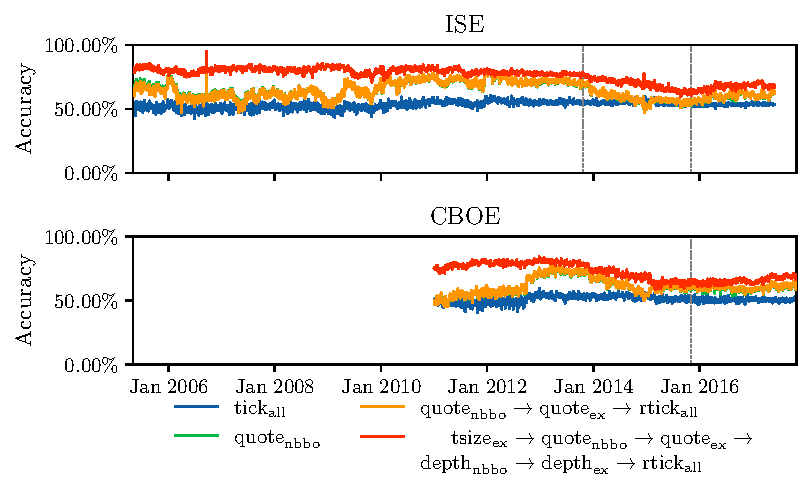
\includegraphics{classical-accuracies-over-time.pdf}
    \caption[Accuracy Of Rule-Based Classifiers On \glsentryshort{ISE} and \glsentryshort{CBOE} Over Time]{Accuracy of rule-based classifiers on \gls{ISE} and \gls{CBOE} sample over time. The dashed bar \myline{} indicates the beginning of a new subset based on the train-test split.}
    \label{fig:classical-accuracies-over-time}
\end{figure}

Aside from these high-level observations, we focus on three findings in greater detail.

\textbf{Finding 1: Accuracy of Basic Rules Is Downward-Biased by Missingness}
\todo{Add finding}

\textbf{Finding 2: Accuracy Comes From Depth}
\todo{Add finding}

\textbf{Finding 3: Fee Structures Affect Accuracy Over Time}
\todo{Add finding}

\begin{table}[ht]
    \centering
    \caption[Accuracies of Rule-Based Approaches On \glsentryshort{CBOE}]{This table shows the accuracy of common trade classification rules and their variations for option trades on \gls{CBOE} sample. Unclassifiable trades by the respective rule are assigned randomly as buy or sell. Hybrid methods are estimated using trade prices across all exchanges. We report the percentage of classifiable trades and the overall accuracy for subsets based on our train-test split and the entire dataset. The best rule is in \textbf{bold}.}
    \label{tab:cboe-classical}
    \begin{tabular}{lSSSS}
        \toprule
        {}                                     & {Coverage in \%}  & \multicolumn{3}{c}{Accuracy in \%}                                         \\ \cmidrule(lr){2-2}\cmidrule(lr){3-5}
        {Classification Rule}                  & {All}             & {Pre-Test}                         & {Test}            & {All}             \\\midrule
        $\operatorname{tick}_{\mathrm{ex}}$    & 91.4507           & 48.6156                            & 48.9969           & 48.7469           \\
        $\operatorname{rtick}_{\mathrm{ex}}$   & 90.2769           & 51.0857                            & 50.5432           & 50.8989           \\
        $\operatorname{quote}_{\mathrm{ex}}$   & 90.5150           & 62.6661                            & 62.0689           & 62.4605           \\
        $\operatorname{lr}_{\mathrm{ex}}$      & 99.7455           & 62.3106                            & 61.5831           & 62.0602           \\
        $\operatorname{rlr}_{\mathrm{ex}}$     & 99.4584           & 62.7035                            & 61.9898           & 62.4578           \\
        $\operatorname{emo}_{\mathrm{ex}}$     & 97.9601           & 49.3923                            & 48.6489           & 49.1364           \\
        $\operatorname{remo}_{\mathrm{ex}}$    & 97.3242           & 49.8883                            & 49.9529           & 49.9105           \\
        $\operatorname{clnv}_{\mathrm{ex}}$    & 98.4350           & 54.2644                            & 53.2492           & 53.9149           \\
        $\operatorname{rclnv}_{\mathrm{ex}}$   & 98.0358           & 55.1506                            & 54.5686           & 54.9502           \\\addlinespace
        $\operatorname{tick}_{\mathrm{all}}$   & 97.2135           & 51.4199                            & 50.4403           & 51.0827           \\
        $\operatorname{rtick}_{\mathrm{all}}$  & 96.0292           & 54.2521                            & 52.7056           & 53.7197           \\\addlinespace
        $\operatorname{quote}_{\mathrm{nbbo}}$ & 91.1772           & 61.3222                            & 59.8123           & 60.8024           \\
        $\operatorname{lr}_{\mathrm{nbbo}}$    & 99.7705           & 60.9503                            & 59.3730           & 60.4073           \\
        $\operatorname{rlr}_{\mathrm{nbbo}}$   & 99.6335           & 61.3095                            & 59.7608           & 60.7764           \\
        $\operatorname{emo}_{\mathrm{nbbo}}$   & 98.7186           & 51.6420                            & 51.6299           & 51.6378           \\
        $\operatorname{remo}_{\mathrm{nbbo}}$  & 98.3939           & 52.4847                            & 53.0736           & 52.6874           \\
        $\operatorname{clnv}_{\mathrm{nbbo}}$  & 98.8975           & 55.3058                            & 54.1294           & 54.9008           \\
        $\operatorname{rclnv}_{\mathrm{nbbo}}$ & 98.7000           & 56.3217                            & 55.4032           & 56.0055           \\\addlinespace
        $\operatorname{gsu}_{\mathrm{small}}$  & 99.7918           & 61.8938                            & 60.7464           & 61.4988           \\
        $\operatorname{gsu}_{\mathrm{large}}$  & \bfseries 99.9943 & \bfseries 74.6511                  & \bfseries 66.5176 & \bfseries 71.8510 \\\bottomrule
    \end{tabular}
\end{table}

We repeat the analysis on the \gls{CBOE} dataset in \cref{tab:cboe-classical} and observe a similar ranking to \cref{tab:ise-classical}. Overall, the performance of classical trade classification rules further diminishes or remains at a low level strengthening the need for alternative classifiers. Tick-based rules trail the performance of quote-based approaches, and the accuracy of hybrids varies with the dependence on the tick test. Different from the \gls{ISE} sample, the quote rule estimated on the \gls{NBBO}, $\operatorname{quote}_{\mathrm{nbbo}}$, leads to a lower performance than the quote rule applied to \gls{CBOE} quotes.
% Parts of this is due to the fact, that  $\operatorname{quote}_{\mathrm{nbbo}}$ achieves a considerably lower coverage of \SI{94.77}{\percent} compared to \SI{99.89}{\percent} in the \gls{ISE} sample, with fewer trades classified by the fallback criterion. In a filtered common sample, where trades are classified by both rules, performance is approximately similar. 
Again, $\operatorname{gsu}_{\mathrm{small}}$ and $\operatorname{gsu}_{\mathrm{large}}$ perform best, the strong outperformance does not carry over to the test set as depicted \cref{fig:classical-accuracies-over-time}.\footnote{Performance on \gls{CBOE} can be improved if the order of quote rules is reversed. For full combinatoric coverage see \textcite[][33]{grauerOptionTradeClassification2022}. To avoid overfitting the test set by classical rules, we keep the baseline constant following our reasoning from \cref{sec:hyperparameter-tuning}.}

\todo{Doesn't this contradict the hidden order idea of Grauer?}

Next, we test the supervised classifiers on the \gls{ISE}/\gls{CBOE} test sets, which prove to be a challenging test ground for rule-based classifiers as our results from above indicate.

\subsection{Results of Supervised
    Models}\label{sec:results-of-supervised-models}

Next, we test the performance of our supervised models. We take the best configurations from \cref{sec:hyperparameter-tuning}, trained and tuned on the \gls{ISE} trade data, and evaluate their performance on the \gls{ISE} and \gls{CBOE} test sets. \cref{tab:results-supervised-ise-cboe} summarizes the results and benchmarks against state-of-the-art solutions from the literature.

\begin{table}[ht]
    \centering
    \caption[Accuracies of Supervised Approaches On \glsentryshort{CBOE} and \glsentryshort{ISE} Dataset]{This table reports the accuracy of supervised \glspl{GBRT} and Transformers for different feature combinations on the \gls{ISE} and \gls{CBOE} datasets. The improvement is estimated as the absolute change in accuracy between the classifier and the benchmark. For feature set classical, $\operatorname{gsu}_{\mathrm{small}}$ is the benchmark and otherwise $\operatorname{gsu}_{\mathrm{large}}$. Models are trained on the \gls{ISE} training set. The best classifier per dataset is in \textbf{bold}.}
    \label{tab:results-supervised-ise-cboe}
    \begin{tabular}{@{}llSSSSSS@{}}
        \toprule
                   &             & \multicolumn{2}{c}{FS Classical} & \multicolumn{2}{c}{FS Classical-Size} & \multicolumn{2}{c}{FS Option}                                                                 \\ \cmidrule(lr){3-4}\cmidrule(lr){5-6} \cmidrule(lr){7-8}
        Dataset    & Classifier  & {Acc. in \%}                     & {+/-}                                 & {Acc. in \%}                  & {+/-}              & {Acc. in \%}        & {+/-}              \\ \midrule
        \gls{ISE}  & \gls{GBRT}  & 63.668637                        & 3.620000                              & 72.343640                     & 4.730000           & \bfseries 74.120496 & \bfseries 6.510000 \\
                   & Transformer & \bfseries 63.783020              & \bfseries 3.730000                    & \bfseries 72.581107           & \bfseries 4.970000 & 73.921795           & 6.310000           \\ \addlinespace
        \gls{CBOE} & \gls{GBRT}  & 66.002029                        & 5.260000                              & 71.951794                     & 5.430000           & \bfseries 74.375033 & \bfseries 7.860000 \\
                   & Transformer & \bfseries 66.182348              & \bfseries 5.440000                    & \bfseries 72.153338           & \bfseries 5.640000 & 74.278318           & 7.760000           \\ \bottomrule
    \end{tabular}
\end{table}

Both model architectures consistently outperform their respective benchmarks on the \gls{ISE} and \gls{CBOE} datasets, achieving state-of-the-art performance in option trade classification with comparable data requirements. Thereby, Transformers dominate the \gls{ISE} sample when trained on trade prices and quotes reaching \SI{63.783020}{\percent}  in accuracy and \SI{66.18}{\percent} on the \gls{CBOE} sample outperforming previous approaches by \SI{3.730000}{\percent} and \SI{5.440000}{\percent}. Additional trade size features improve the accuracy to \SI{72.581107}{\percent} for the \gls{ISE} sample and \SI{72.153338}{\percent} for the \gls{CBOE} sample. Gradient boosting outperforms all other approaches when trained on additional option features.

While absolute improvements in accuracy over $\operatorname{gsu}_{\mathrm{small}}$ are modest on the smallest feature set, improvements are more substantial for larger feature sets ranging between \SI{4.730000}{\percent} to \SI{7.860000}{\percent} over $\operatorname{gsu}_{\mathrm{large}}$. Specifically, the addition of trade size-related features positively contributes to the performance. The results can be further improved through retraining on the validation set, as documented in \cref{app:results-of-supervised-models-with-re-training}. In favour of conservative estimates, our models in the main text do not use this technique.

Expectedly, performance differences between gradient boosting and Transformers are minor. This result is consistent with \textcites{grinsztajnWhyTreebasedModels2022}{gorishniyRevisitingDeepLearning2021}, who conclude for tabular modelling, that neither Transformers or \gls{GBRT} are universally superior.

Counter-intuitively, performance improvements are highest for the \gls{CBOE} dataset, despite the models being trained on \gls{ISE} data. Part of this is due to a weaker benchmark performance, but also due to a considerably stronger accuracy of classifiers on the smallest and mid-sized feature sets. One would expect a degradation between sets, assuming exchange-specific trading patterns and requiring exploration in greater detail.

% \begin{figure}[!h]
%     \subfloat[tbd\label{fig:confusion-matrix-supervised-cboe}]{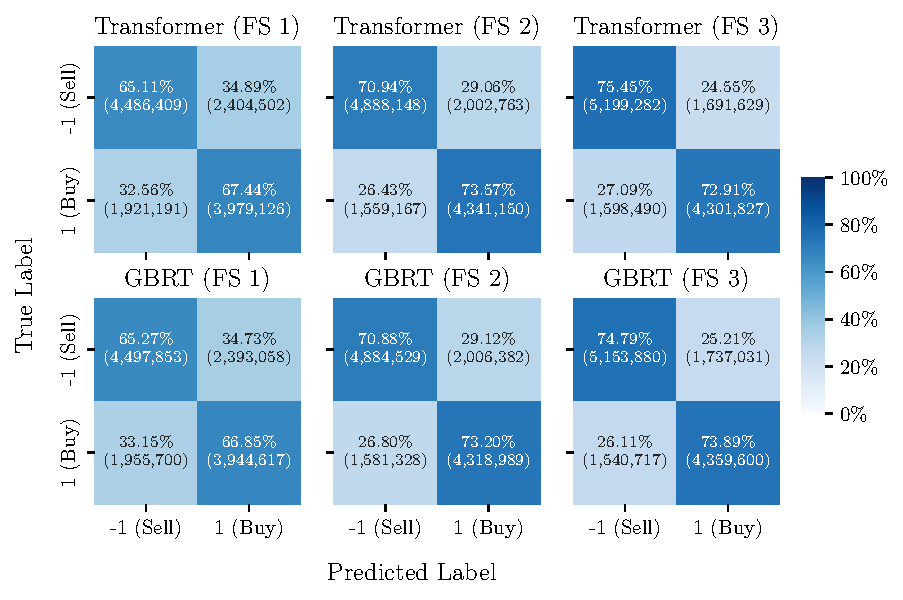
\includegraphics[width=0.8\textwidth]{confusion_matrix_cboe.pdf}}
%     \vfill
%     \subfloat[tbd\label{fig:confusion-matrix-supervised-ise}]{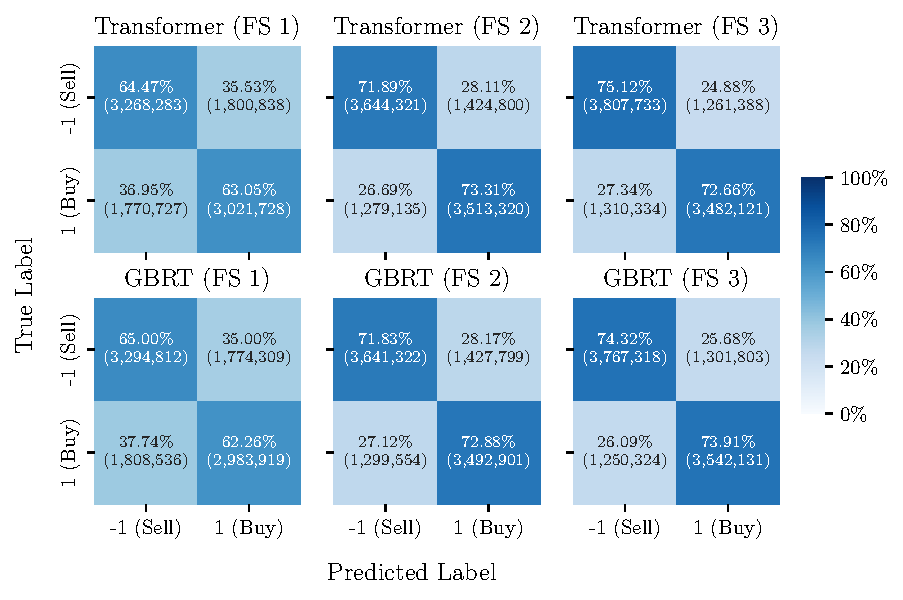
\includegraphics[width=0.8\textwidth]{confusion_matrix_ise.pdf}}
%     \caption[]{Confusion Matrices Of Supervised Classifiers}
%     \label{fig:confusion-matrix-supervised-ise-cboe}
% \end{figure}

\subsection{Results of Semi-Supervised
    Models}\label{sec:results-of-semi-supervised-models}

\begin{table}[ht]
    \centering
    \caption[Accuracies of Semi-Supervised Approaches On \glsentryshort{CBOE} and \glsentryshort{ISE} Dataset]{This table reports the accuracy of semi-supervised \glspl{GBRT} and Transformers for different feature combinations on the \gls{ISE} and \gls{CBOE} datasets. The improvement is estimated as the absolute change in accuracy between the classifier and the benchmark. For feature set classical, $\operatorname{gsu}_{\mathrm{small}}$ is the benchmark and otherwise $\operatorname{gsu}_{\mathrm{large}}$. Models are trained on the \gls{ISE} training set. The best classifier per dataset is in \textbf{bold}.}
    \label{tab:results-semi-supervised-ise-cboe}
    \begin{tabular}{@{}llSSSSSS@{}}
        \toprule
                   &             & \multicolumn{2}{c}{FS Classical} & \multicolumn{2}{c}{FS Classical-Size} & \multicolumn{2}{c}{FS Option}                                \\ \cmidrule(lr){3-4}\cmidrule(lr){5-6} \cmidrule(lr){7-8}
        Dataset    & Classifier  & {Acc. in \%}                     & {+/-}                                 & {Acc. in \%}                  & {+/-} & {Acc. in \%} & {+/-} \\ \midrule
        \gls{ISE}  & \gls{GBRT}  & 63.397514 & 3.350000 & 72.156489 & 4.550000 & 73.536644 & 5.930000 \\
                   & Transformer &                                  &                                       &                               &       &              &       \\ \addlinespace
        \gls{CBOE} & \gls{GBRT}  & 66.189454 & 5.440000 & 71.922680 & 5.410000 & 73.953322 & 7.440000 \\
                   & Transformer &                                  &                                       &                               &       &              &       \\ \bottomrule
    \end{tabular}
\end{table}

\subsection{Robustness of Results}\label{sec:robustness-checks}

\todo{Again, results are not 100 \% comparaable due to grouping.}
\todo{Compare improvements with other works. Improvments much greater than ronen et al. }

\textbf{Gradient Boosting}

\begin{table}[ht]
    \centering
    \caption[short-diff-ise-supervised-test-gbm]{long-diff-ise-supervised-test-gbm}
    \label{tab:diff-ise_supervised_test}
    \begin{tabular}{lSSSSSS@{}}
        \toprule
        {}                       & \multicolumn{2}{c}{FS Classical} & \multicolumn{2}{c}{FS Classical-Size} & \multicolumn{2}{c}{FS Option}                                        \\ \cmidrule(lr){2-3}\cmidrule(lr){4-5}\cmidrule(lr){6-7}
        {}                       & {Acc. in \%}                     & {+/-}                                 & {Acc. in \%}                  & {+/-}     & {Acc. in \%} & {+/-}     \\\midrule
        \multicolumn{7}{l}{ Option Type}                                                                                                                                           \\
        \tabindent  C            & 62.890486                        & 3.720000                              & 71.884647                     & 4.480000  & 73.647971    & 6.240000  \\
        \tabindent  P            & 64.557394                        & 3.500000                              & 72.867874                     & 5.020000  & 74.660185    & 6.820000  \\
        \cmidrule(rl){1-7}
        \multicolumn{7}{l}{ Security Type}                                                                                                                                         \\
        \tabindent  Index option & 56.345043                        & -1.460000                             & 57.474458                     & -1.020000 & 58.649239    & 0.150000  \\
        \tabindent Others        & 68.399095                        & 2.870000                              & 76.369535                     & 5.790000  & 77.590573    & 7.010000  \\
        \tabindent Stock Option  & 61.877752                        & 4.000000                              & 70.946999                     & 4.400000  & 72.956919    & 6.410000  \\
        \cmidrule(rl){1-7}
        \multicolumn{7}{l}{ Trade Size}                                                                                                                                            \\
        \tabindent (0,1]         & 61.892029                        & 3.350000                              & 72.564793                     & 3.390000  & 74.245655    & 5.070000  \\
        \tabindent  (1,3]        & 62.473959                        & 4.020000                              & 72.965377                     & 3.680000  & 74.857610    & 5.570000  \\
        \tabindent  (3,5]        & 62.696932                        & 3.890000                              & 72.755628                     & 3.360000  & 74.647279    & 5.250000  \\
        \tabindent  (5,11]       & 65.928967                        & 3.380000                              & 71.752039                     & 8.080000  & 73.450299    & 9.780000  \\
        \tabindent  >11          & 67.310266                        & 3.640000                              & 71.337373                     & 6.380000  & 73.145472    & 8.190000  \\
        \cmidrule(rl){1-7}
        \multicolumn{7}{l}{ Year}                                                                                                                                                  \\
        \tabindent 2015          & 60.446922                        & 4.050000                              & 69.000296                     & 5.210000  & 71.512360    & 7.730000  \\
        \tabindent  2016         & 63.736474                        & 3.560000                              & 72.555638                     & 5.030000  & 74.290527    & 6.770000  \\
        \tabindent  2017         & 64.596306                        & 3.610000                              & 72.977560                     & 3.870000  & 74.604216    & 5.500000  \\
        \cmidrule(rl){1-7}
        \multicolumn{7}{l}{ Time To Maturity}                                                                                                                                      \\
        \tabindent  <= 1         & 64.458297                        & 3.580000                              & 72.756774                     & 5.240000  & 74.604553    & 7.090000  \\
        \tabindent  (1-2]        & 64.612677                        & 3.800000                              & 72.869099                     & 4.300000  & 73.947396    & 5.370000  \\
        \tabindent (2-3]         & 63.015912                        & 3.110000                              & 71.743691                     & 3.460000  & 72.997282    & 4.710000  \\
        \tabindent  (3-6]        & 61.788369                        & 3.640000                              & 71.288086                     & 3.430000  & 72.750293    & 4.890000  \\
        \tabindent  (6-12]       & 61.911555                        & 3.990000                              & 71.199996                     & 3.310000  & 73.130453    & 5.240000  \\
        \tabindent  > 12         & 55.126547                        & 3.830000                              & 68.572852                     & 3.540000  & 72.004951    & 6.980000  \\
        \cmidrule(rl){1-7}
        \multicolumn{7}{l}{ Moneyness}                                                                                                                                             \\
        \tabindent  <= 0.7       & 65.531247                        & 3.790000                              & 71.917341                     & 7.520000  & 72.307517    & 7.910000  \\
        \tabindent  (0.7-0.9]    & 67.642270                        & 3.670000                              & 74.254665                     & 5.960000  & 75.433765    & 7.140000  \\
        \tabindent  (0.9-1.1]    & 64.059687                        & 3.530000                              & 72.975308                     & 4.400000  & 74.457482    & 5.880000  \\
        \tabindent  (1.1-1.3]    & 54.294722                        & 4.040000                              & 66.220667                     & 4.190000  & 70.375579    & 8.350000  \\
        \tabindent  > 1.3        & 52.623795                        & 3.770000                              & 63.075529                     & 2.870000  & 70.489510    & 10.280000 \\
        \cmidrule(rl){1-7}
        \multicolumn{7}{l}{ Proximity To Quotes}                                                                                                                                   \\
        \tabindent  At Mid       & 62.644890                        & 5.490000                              & 72.164951                     & 4.020000  & 74.685118    & 6.540000  \\
        \tabindent  Inside       & 62.605233                        & 2.160000                              & 68.301819                     & 3.800000  & 70.295127    & 5.790000  \\
        \tabindent  At Quotes    & 67.828443                        & 7.860000                              & 86.667541                     & 8.450000  & 87.313763    & 9.100000  \\
        \tabindent  Outside      & 61.350064                        & -5.430000                             & 61.846608                     & -3.070000 & 64.034087    & -0.890000 \\
        \tabindent  Unknown      & 78.638385                        & 2.230000                              & 78.275744                     & 1.870000  & 78.816285    & 2.410000  \\
        \cmidrule(rl){1-7}
        \multicolumn{7}{l}{ All}                                                                                                                                                   \\
        \tabindent  All          & 63.668637                        & 3.620000                              & 72.343640                     & 4.730000  & 74.120496    & 6.510000  \\
        \bottomrule
    \end{tabular}
\end{table}



\begin{table}[ht]
    \centering
    \caption[short-diff-cboe-transfer-test]{long-diff-cboe-gbm-tbd}
    \label{tab:diff-cboe_transfer-gbm}
    \begin{tabular}{lSSSSSS@{}}
        \toprule
        {}                      & \multicolumn{2}{c}{FS Classical} & \multicolumn{2}{c}{FS Classical-Size} & \multicolumn{2}{c}{FS Option}                                        \\ \cmidrule(lr){2-3}\cmidrule(lr){4-5}\cmidrule(lr){6-7}
        {}                      & {Acc. in \%}                     & {+/-}                                 & {Acc. in \%}                  & {+/-}     & {Acc. in \%} & {+/-}     \\\midrule
        \multicolumn{7}{l}{ Option Type}                                                                                                                                          \\
        \tabindent C            & 65.505083                        & 5.370000                              & 71.707057                     & 5.770000  & 74.283388    & 8.350000  \\
        \tabindent P            & 66.597419                        & 5.120000                              & 72.245014                     & 5.030000  & 74.484832    & 7.270000  \\
        \cmidrule(rl){1-7}
        \multicolumn{7}{l}{Security Type}                                                                                                                                         \\
        \tabindent Index Option & 60.365562                        & 7.070000                              & 67.298912                     & 0.850000  & 72.394792    & 5.940000  \\
        \tabindent Others       & 69.054857                        & 4.420000                              & 74.137168                     & 5.210000  & 75.534837    & 6.610000  \\
        \tabindent Stock Option & 65.293961                        & 5.420000                              & 71.506273                     & 5.980000  & 74.089988    & 8.570000  \\
        \cmidrule(rl){1-7}
        \multicolumn{7}{l}{ Trade Size}                                                                                                                                           \\
        \tabindent (0,1]        & 62.831155                        & 5.860000                              & 70.756340                     & 6.780000  & 73.423543    & 9.450000  \\
        \tabindent (1,3]        & 64.895723                        & 5.200000                              & 71.318816                     & 6.330000  & 73.634574    & 8.640000  \\
        \tabindent (3,5]        & 65.549362                        & 5.060000                              & 71.956770                     & 5.620000  & 74.174579    & 7.840000  \\
        \tabindent(5,11]        & 66.577620                        & 5.150000                              & 71.566680                     & 5.170000  & 74.143799    & 7.750000  \\
        \tabindent >11          & 71.136074                        & 4.750000                              & 74.549126                     & 2.830000  & 76.765762    & 5.050000  \\
        \cmidrule(rl){1-7}
        \multicolumn{7}{l}{Year}                                                                                                                                                  \\                                                                                                                                        \\
        \tabindent 2015         & 65.689585                        & 4.460000                              & 71.445193                     & 6.400000  & 74.317847    & 9.270000  \\
        \tabindent 2016         & 65.579978                        & 5.350000                              & 71.638148                     & 6.430000  & 74.178699    & 8.970000  \\
        \tabindent 2017         & 66.491658                        & 5.250000                              & 72.349451                     & 4.250000  & 74.591947    & 6.500000  \\
        \cmidrule(rl){1-7}
        \multicolumn{7}{l}{ Time To Maturity}                                                                                                                                     \\
        \tabindent <= 1         & 66.863272                        & 4.940000                              & 72.005520                     & 5.140000  & 74.272153    & 7.410000  \\
        \tabindent (1-2]        & 67.553775                        & 5.590000                              & 72.584599                     & 5.170000  & 75.237684    & 7.820000  \\
        \tabindent (2-3]        & 66.061857                        & 5.770000                              & 72.349461                     & 5.110000  & 74.713903    & 7.480000  \\
        \tabindent (3-6]        & 65.007308                        & 5.950000                              & 72.855935                     & 6.220000  & 75.086134    & 8.450000  \\
        \tabindent (6-12]       & 64.184403                        & 5.600000                              & 71.908786                     & 6.200000  & 74.389885    & 8.690000  \\
        \tabindent > 12         & 56.065976                        & 5.380000                              & 66.802260                     & 7.160000  & 71.092148    & 11.450000 \\
        \cmidrule(rl){1-7}
        \multicolumn{7}{l}{ Moneyness}                                                                                                                                            \\
        \tabindent <= 0.7       & 65.722320                        & 5.400000                              & 72.842929                     & 3.880000  & 75.645703    & 6.680000  \\
        \tabindent (0.7-0.9]    & 66.272446                        & 5.460000                              & 72.187575                     & 5.130000  & 74.768887    & 7.710000  \\
        \tabindent (0.9-1.1]    & 66.977290                        & 5.190000                              & 72.619255                     & 5.420000  & 74.739508    & 7.540000  \\
        \tabindent (1.1-1.3]    & 58.197013                        & 5.020000                              & 66.153817                     & 7.100000  & 69.833429    & 10.780000 \\
        \tabindent > 1.3        & 56.958403                        & 5.890000                              & 64.569317                     & 6.580000  & 70.478616    & 12.490000 \\
        \cmidrule(rl){1-7}
        \multicolumn{7}{l}{ Proximity To Quotes}                                                                                                                                  \\
        \tabindent At Mid       & 60.688727                        & 6.950000                              & 67.528635                     & 4.080000  & 69.104800    & 5.660000  \\
        \tabindent Inside       & 68.822448                        & 3.030000                              & 71.987785                     & 6.150000  & 73.698272    & 7.860000  \\
        \tabindent At Quotes    & 54.187224                        & 16.010000                             & 74.756821                     & 2.410000  & 81.426352    & 9.080000  \\
        \tabindent Outside      & 70.719978                        & -4.200000                             & 70.369607                     & -1.560000 & 69.648255    & -2.280000 \\
        \tabindent Unknown      & 83.771336                        & 1.110000                              & 83.608778                     & 0.950000  & 84.213854    & 1.550000  \\
        \cmidrule(rl){1-7}
        \multicolumn{7}{l}{ All}                                                                                                                                                  \\
        \tabindent All          & 66.002029                        & 5.260000                              & 71.951794                     & 5.430000  & 74.375033    & 7.860000  \\
        \bottomrule
    \end{tabular}
\end{table}


\textbf{FT-Transformer}

\begin{table}[ht]
    \centering
    \caption[short-diff-ise-supervised-test-fttransformer]{long-diff-ise-supervised-test-fttransformer}
    \label{tab:diff-ise_supervised-test}
    \begin{tabular}{lSSSSSS@{}}
        \toprule
        {}                      & \multicolumn{2}{c}{FS Classical} & \multicolumn{2}{c}{FS Classical-Size} & \multicolumn{2}{c}{FS Option}                                        \\ \cmidrule(lr){2-3}\cmidrule(lr){4-5}\cmidrule(lr){6-7}
        {}                      & {Acc. in \%}                     & {+/-}                                 & {Acc. in \%}                  & {+/-}     & {Acc. in \%} & {+/-}     \\\midrule
        \multicolumn{7}{l}{ Option Type}                                                                                                                                          \\
        \tabindent C            & 62.991514                        & 3.820000                              & 72.099064                     & 4.690000  & 73.484904    & 6.080000  \\
        \tabindent P            & 64.687031                        & 3.630000                              & 73.131667                     & 5.290000  & 74.420786    & 6.580000  \\
        \cmidrule(rl){1-7}
        \multicolumn{7}{l}{ Security Type}                                                                                                                                        \\
        \tabindent Index option & 56.519890                        & -1.290000                             & 58.457380                     & -0.040000 & 58.641678    & 0.140000  \\
        \tabindent Others       & 68.443599                        & 2.920000                              & 76.549050                     & 5.970000  & 77.590109    & 7.010000  \\
        \tabindent Stock option & 62.019384                        & 4.140000                              & 71.196166                     & 4.650000  & 72.674763    & 6.120000  \\
        \cmidrule(rl){1-7}
        \multicolumn{7}{l}{ Trade Size}                                                                                                                                           \\
        \tabindent (0,1]        & 62.127137                        & 3.590000                              & 72.877007                     & 3.710000  & 73.967386    & 4.800000  \\
        \tabindent (1,3]        & 62.654716                        & 4.200000                              & 73.321548                     & 4.040000  & 74.721308    & 5.440000  \\
        \tabindent (3,5]        & 62.839285                        & 4.030000                              & 73.161769                     & 3.770000  & 74.715927    & 5.320000  \\
        \tabindent (5,11]       & 65.756057                        & 3.200000                              & 71.877263                     & 8.210000  & 73.441354    & 9.770000  \\
        \tabindent >11          & 67.380602                        & 3.710000                              & 71.237293                     & 6.280000  & 72.584805    & 7.630000  \\
        \cmidrule(rl){1-7}
        \multicolumn{7}{l}{ Year}                                                                                                                                                 \\
        \tabindent 2015         & 60.620179                        & 4.220000                              & 69.609946                     & 5.820000  & 71.861077    & 8.070000  \\
        \tabindent 2016         & 63.851905                        & 3.680000                              & 72.798245                     & 5.270000  & 74.138951    & 6.620000  \\
        \tabindent 2017         & 64.688426                        & 3.700000                              & 73.077731                     & 3.970000  & 74.111711    & 5.010000  \\
        \cmidrule(rl){1-7}
        \multicolumn{7}{l}{ Time To Maturity}                                                                                                                                     \\
        \tabindent <= 1         & 64.546416                        & 3.670000                              & 72.976628                     & 5.460000  & 74.450445    & 6.930000  \\
        \tabindent (1-2]        & 64.736461                        & 3.930000                              & 73.043470                     & 4.470000  & 73.692560    & 5.120000  \\
        \tabindent(2-3]         & 63.152545                        & 3.250000                              & 72.063690                     & 3.780000  & 72.896064    & 4.610000  \\
        \tabindent (3-6]        & 61.887659                        & 3.740000                              & 71.531191                     & 3.670000  & 72.287641    & 4.420000  \\
        \tabindent (6-12]       & 62.021518                        & 4.100000                              & 71.325950                     & 3.430000  & 72.466903    & 4.570000  \\
        \tabindent > 12         & 55.669126                        & 4.380000                              & 69.313656                     & 4.290000  & 72.282466    & 7.250000  \\
        \cmidrule(rl){1-7}
        \multicolumn{7}{l}{ Moneyness}                                                                                                                                            \\
        \tabindent <= 0.7       & 65.196444                        & 3.460000                              & 71.762641                     & 7.370000  & 71.689001    & 7.290000  \\
        \tabindent (0.7-0.9]    & 67.618182                        & 3.650000                              & 74.318808                     & 6.030000  & 74.876535    & 6.580000  \\
        \tabindent (0.9-1.1]    & 64.141472                        & 3.610000                              & 73.115683                     & 4.540000  & 74.236648    & 5.660000  \\
        \tabindent (1.1-1.3]    & 54.943206                        & 4.690000                              & 67.505754                     & 5.480000  & 70.929706    & 8.900000  \\
        \tabindent > 1.3        & 53.468351                        & 4.620000                              & 64.293219                     & 4.080000  & 71.424038    & 11.210000 \\
        \cmidrule(rl){1-7}
        \multicolumn{7}{l}{ Proximity To Quotes}                                                                                                                                  \\
        \tabindent At Mid       & 62.490146                        & 5.340000                              & 72.138236                     & 3.990000  & 74.022892    & 5.870000  \\
        \tabindent Inside       & 62.566010                        & 2.120000                              & 68.807735                     & 4.300000  & 70.429973    & 5.930000  \\
        \tabindent At Quotes    & 68.608870                        & 8.640000                              & 86.087938                     & 7.870000  & 86.165327    & 7.950000  \\
        \tabindent Outside      & 63.228880                        & -3.550000                             & 63.792525                     & -1.130000 & 65.610951    & 0.690000  \\
        \tabindent Unknown      & 78.268902                        & 1.860000                              & 77.824153                     & 1.420000  & 78.522066    & 2.110000  \\
        \cmidrule(rl){1-7}
        \multicolumn{7}{l}{ All}                                                                                                                                                  \\
        \tabindent All          & 63.783020                        & 3.730000                              & 72.581107                     & 4.970000  & 73.921795    & 6.310000  \\
        \bottomrule
    \end{tabular}
\end{table}

\begin{table}[ht]
    \centering
    \caption[short-diff-cboe-transfer-test-fttransformer]{long-diff-cboe-transfer-test-fttransformer}
    \label{tab:diff-cboe_transfer_test}
    \begin{tabular}{lSSSSSS@{}}
        \toprule
        {}                      & \multicolumn{2}{c}{FS Classical} & \multicolumn{2}{c}{FS Classical-Size} & \multicolumn{2}{c}{FS Option}                                       \\ \cmidrule(lr){2-3}\cmidrule(lr){4-5}\cmidrule(lr){6-7}
        {}                      & {Acc. in \%}                     & {+/-}                                 & {Acc. in \%}                  & {+/-}    & {Acc. in \%} & {+/-}     \\\midrule
        \multicolumn{7}{l}{ Option Type}                                                                                                                                         \\
        \tabindent C            & 65.628907                        & 5.490000                              & 71.945453                     & 6.010000 & 74.579113    & 8.640000  \\
        \tabindent P            & 66.845425                        & 5.370000                              & 72.402406                     & 5.190000 & 73.917935    & 6.700000  \\
        \cmidrule(rl){1-7}
        \multicolumn{7}{l}{ Security Type}                                                                                                                                       \\
        \tabindent Index option & 61.207800                        & 7.910000                              & 67.170125                     & 0.720000 & 69.051358    & 2.600000  \\
        \tabindent Others       & 69.266211                        & 4.630000                              & 74.427252                     & 5.500000 & 75.859396    & 6.940000  \\
        \tabindent Stock option & 65.395694                        & 5.520000                              & 71.703855                     & 6.180000 & 74.141068    & 8.620000  \\
        \cmidrule(rl){1-7}
        \multicolumn{7}{l}{ Trade Size}                                                                                                                                          \\
        \tabindent (0,1]        & 63.135782                        & 6.170000                              & 71.074930                     & 7.100000 & 73.362654    & 9.380000  \\
        \tabindent (1,3]        & 64.993995                        & 5.300000                              & 71.513064                     & 6.520000 & 73.846381    & 8.860000  \\
        \tabindent (3,5]        & 65.605000                        & 5.110000                              & 72.070498                     & 5.730000 & 74.237799    & 7.900000  \\
        \tabindent (5,11]       & 66.701471                        & 5.280000                              & 71.890991                     & 5.490000 & 73.979636    & 7.580000  \\
        \tabindent >11          & 71.378727                        & 4.990000                              & 74.552019                     & 2.840000 & 76.246445    & 4.530000  \\
        \cmidrule(rl){1-7}
        \multicolumn{7}{l}{ Year}                                                                                                                                                \\
        \tabindent 2015         & 65.830149                        & 4.600000                              & 71.843643                     & 6.800000 & 74.755266    & 9.710000  \\
        \tabindent 2016         & 65.786999                        & 5.560000                              & 71.935076                     & 6.720000 & 74.353864    & 9.140000  \\
        \tabindent 2017         & 66.648330                        & 5.410000                              & 72.424788                     & 4.330000 & 74.138831    & 6.040000  \\
        \cmidrule(rl){1-7}
        \multicolumn{7}{l}{ Time To Maturity}                                                                                                                                    \\
        \tabindent <= 1         & 66.927563                        & 5.000000                              & 72.081695                     & 5.220000 & 74.167407    & 7.310000  \\
        \tabindent (1-2]        & 67.642166                        & 5.680000                              & 72.576488                     & 5.160000 & 74.914699    & 7.500000  \\
        \tabindent (2-3]        & 66.550561                        & 6.250000                              & 72.383470                     & 5.150000 & 73.512089    & 6.280000  \\
        \tabindent (3-6]        & 65.257500                        & 6.200000                              & 73.243404                     & 6.610000 & 75.241041    & 8.610000  \\
        \tabindent (6-12]       & 64.630833                        & 6.050000                              & 72.430785                     & 6.730000 & 74.759232    & 9.050000  \\
        \tabindent > 12         & 56.949258                        & 6.270000                              & 68.451314                     & 8.810000 & 71.975430    & 12.340000 \\
        \cmidrule(rl){1-7}
        \multicolumn{7}{l}{ Moneyness}                                                                                                                                           \\
        \tabindent <= 0.7       & 65.747181                        & 5.420000                              & 72.938769                     & 3.980000 & 75.030310    & 6.070000  \\
        \tabindent (0.7-0.9]    & 66.501088                        & 5.690000                              & 72.160406                     & 5.100000 & 73.928341    & 6.870000  \\
        \tabindent (0.9-1.1]    & 67.105536                        & 5.320000                              & 72.698844                     & 5.500000 & 74.754866    & 7.560000  \\
        \tabindent (1.1-1.3]    & 58.732468                        & 5.550000                              & 67.827369                     & 8.770000 & 70.847531    & 11.790000 \\
        \tabindent > 1.3        & 57.597394                        & 6.530000                              & 66.397443                     & 8.400000 & 71.088957    & 13.100000 \\
        \cmidrule(rl){1-7}
        \multicolumn{7}{l}{ Proximity To Quotes}                                                                                                                                 \\
        \tabindent At Mid       & 60.688727                        & 6.950000                              & 67.528635                     & 4.080000 & 69.104800    & 5.660000  \\
        \tabindent Inside       & 68.679525                        & 2.890000                              & 72.284311                     & 6.440000 & 73.930387    & 8.090000  \\
        \tabindent At Quotes    & 56.479734                        & 18.300000                             & 74.815580                     & 2.470000 & 79.999142    & 7.650000  \\
        \tabindent Outside      & 73.145095                        & -1.770000                             & 72.581753                     & 0.650000 & 71.908491    & -0.020000 \\
        \tabindent Unknown      & 83.807460                        & 1.150000                              & 83.220446                     & 0.560000 & 83.491375    & 0.830000  \\
        \cmidrule(rl){1-7}
        \multicolumn{7}{l}{ All}                                                                                                                                                 \\
        \tabindent All          & 66.182348                        & 5.440000                              & 72.153338                     & 5.640000 & 74.278318    & 7.760000  \\
        \bottomrule
    \end{tabular}
\end{table}

\todo{When the analysis was repeated using only the Lee and Radhakrishna subsample, the results were equally as strong or stronger, with two exceptions. Using their subsample, time between transactions is no longer a statistically signi"cant determinant of misclassi"cation and large trades are misclassi"ed slightly more frequently than small trades (odderswhite)}
\todo{Our focus is on ... rules.}
\todo{Improvements are particularily high for trades that are notourisly hard to classify by classical trade classification algorithms.}

\subsection{Feature Importance}\label{sec:feature-importance}

\textbf{Sage Values}

\begin{figure}[ht]
    \centering
    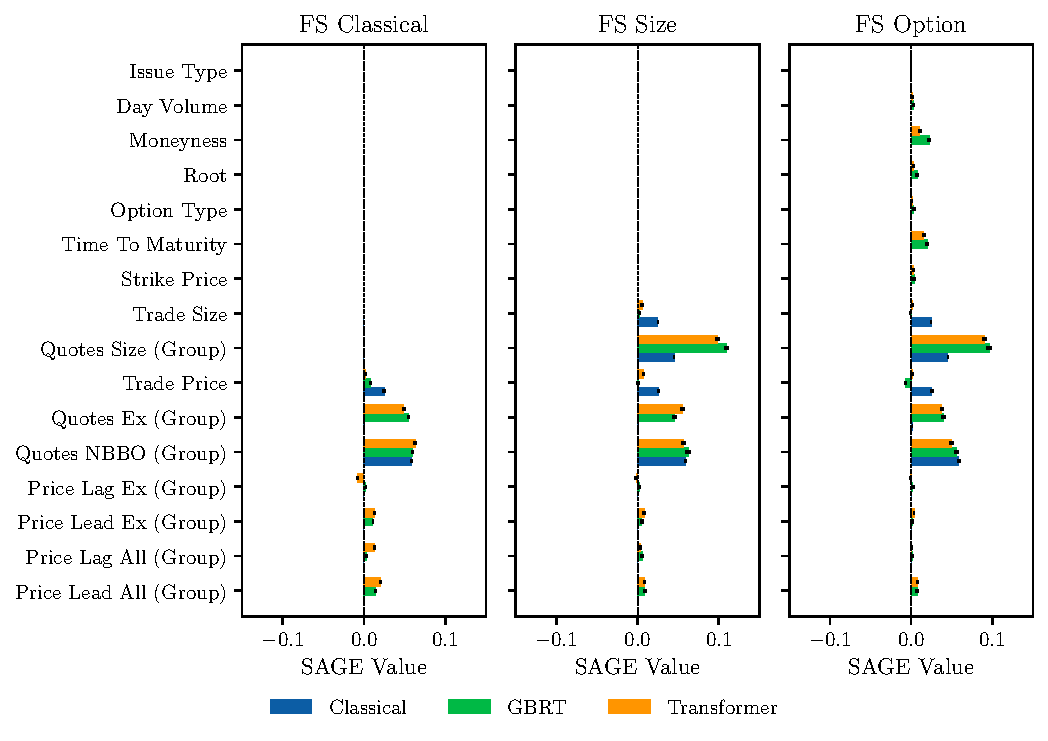
\includegraphics[width=1\textwidth]{sage-importances.pdf}
    \caption[tbd]{tbd}
    \label{fig:sage-importances}
\end{figure}

\textbf{Attention Maps}

\textbf{Categorical Embeddings}

\begin{figure}[!ht]
    \subfloat[Most Similar Embeddings to $\mathtt{SPY}$\label{fig:cat-embeddings-spy}]{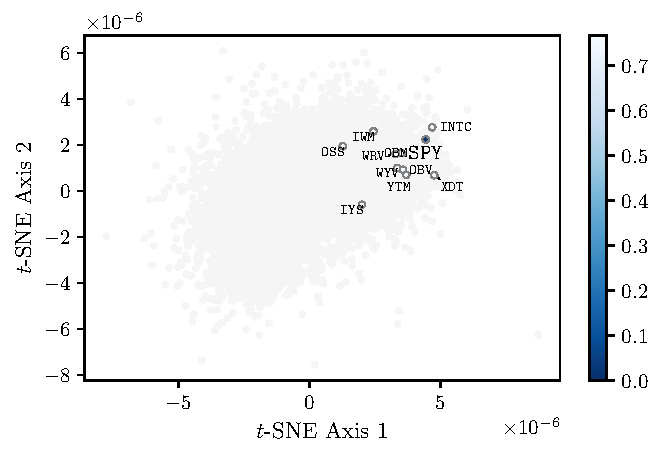
\includegraphics[width=0.6\textwidth]{categorical_embeddings_SPY.pdf}}
    \vfill
    \subfloat[Most Similar Embeddings to $\mathtt{JPM}$\label{fig:fig:cat-embeddings-jpm}]{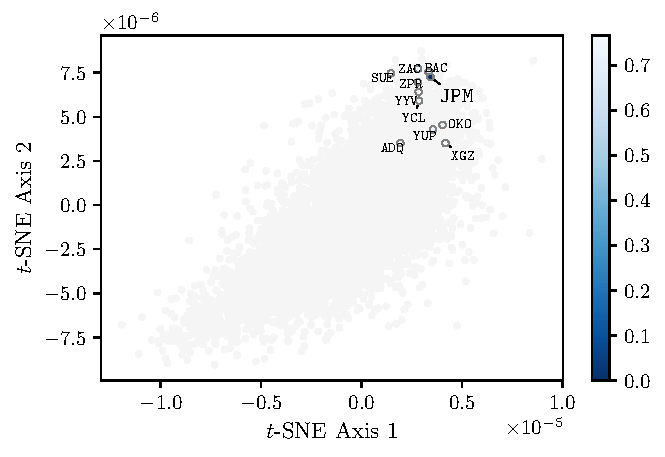
\includegraphics[width=0.6\textwidth]{categorical_embeddings_JPM.pdf}}
    \vfill
    % \subfloat[Most Similar Embeddings to $\mathtt{XOM}$\label{fig:fig:cat-embeddings-xom}]{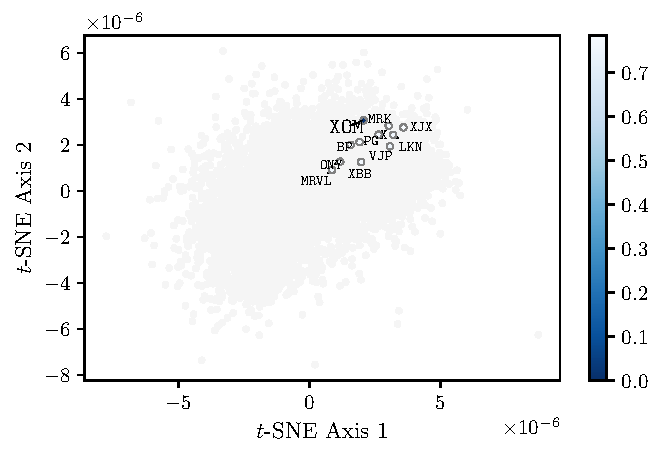
\includegraphics[width=0.6\textwidth]{categorical_embeddings_XOM.pdf}}
    % Exxon Mobil Corporation ($\mathtt{XOM}$)    
    \caption[Categorical Embeddings of Selected Underlyings]{Categorical embeddings of selected underlyings. The plot depicts the projected embedding of SPDR S\&P 500 Trust ($\mathtt{SPY}$) and JPMorgan Chase \& Co ($\mathtt{JPM}$) and their most similar embeddings. Embeddings are projected into 2D-space using $t$-SNE \autocite{vandermaatenVisualizingDataUsing2008}. The ten most similar embeddings by cosine similarity in the original space are coloured and annotated. Distance in projected space is not relevant.}
    \label{fig:categorical-embeddings}
\end{figure}

\todo{Add more examples. Link to online visualisation \url{https://docs.wandb.ai/guides/app/features/panels/weave/embedding-projector}
}




\newpage
\section{Application in Transaction Cost Estimation}\label{sec:application}

\textbf{Preliminaries}

% TODO: Add why it is important. See Stoll, Huang, Roll (zettelkasten)

Albeit the classification accuracy is a reasonable measure for comparing classifiers, one cannot immediately infer how changes in accuracy e.~g., an improvement by \SI{1}{\percent}, affect the application domains. In an attempt to make our results tangible, we apply all algorithms to estimate trading cost, a problem we previously identified to be reliant on correct trade classification (cp. \cref{sec:introduction}) and a common testing ground for trade classification rules \autocites[cp.][541]{ellisAccuracyTradeClassification2000}[][569]{finucaneDirectTestMethods2000}[][271--278]{petersonEvaluationBiasesExecution2003}[][896--897]{savickasInferringDirectionOption2003}.

One of the most widely adopted measures for trading costs is the effective spread \autocite[][112]{Piwowar_2006}. It is defined as the difference between the trade price and the fundamental value of the asset \autocite[][238--239]{bessembinderIssuesAssessingTrade2003}. Following \textcite[][238--239]{bessembinderIssuesAssessingTrade2003}, we define the \emph{nominal, effective spread} as
\begin{equation}
    S_{i,t} = 2 (P_{i,t} - V_{i,t}) D_{i,t}.
    \label{eq:effective-spread}
\end{equation}

Like before, $i$ indexes the security and $t$ the point in time. Here, $D_{i,t}$ is the trade direction, which is either $1$ for customer buy orders and $-1$ for sell orders. If the trade initiator is known, we set $D_{i,t} = y_{i,t}$ and $D_{i,t}=\hat{y}_{it}$, if inferred from a rule or classifier. As the fundamental value $V_{i,t}$ is unobserved at the time of the trade, we follow a common track in research and use the midpoint of the prevailing quotes as an observable proxy.\footnote{An alternative treatment for options is discussed in \textcite[][4975--4976]{muravyevOptionsTradingCosts2020} Our focus is on the midspread, as it is the most common proxy for the value.} This is also a natural choice, under the assumption that, on average, the spread is symmetric and centred around the true fundamental value \autocite[][1018]{leeMarketIntegrationPrice1993}. We multiply the so-obtained half-spread by $\times 2$ to obtain the effective spread, which represents the cost for a round trip trade involving a buy and sell excluding commissions.

Apparent from \cref{eq:effective-spread}, poor estimates for the predicted trade direction, lead to an under or overestimated effective spread, and hence to a skewed trade cost estimate. Only for trades at the midspread, the predicted trade direction is irrelevant, since the effective spread is zero. By comparing the true effective spread from the estimated, we can derive the economic significance. For convenience, we also calculate the \emph{relative effective spread} as
\begin{equation}
    {PS}_{i,t} = S_{i,t} / V_{i,t}.
\end{equation}
% FIXME: check how it is defined Savickas / Finucane use midpoint, Peterson and Sirri divide by price / so does chakrabarty 2007 p. 3819?
The subsequent section estimates both the nominal and relative effective spread for our test sets, as well as the quoted spread.

\textbf{Results}

The actual and the estimated effective spreads, as well as the quoted spread, are shown in the \cref{tab:effective-spread} aggregated by mean. \textcite[][896--897]{savickasInferringDirectionOption2003} estimated the effective spreads on a subset of rules for option trades at the \gls{CBOE}, which can be compared against.

\begin{table}[H]
    \centering
    \begin{threeparttable}
    \sisetup{
        round-precision = 3, 
      }
    \begin{tabular}{llSSSS}
        \toprule
        {}                                               & {}   & \multicolumn{2}{c}{\gls{ISE}} & \multicolumn{2}{c}{\gls{CBOE}}                                 \\ \cmidrule(lr){3-4}\cmidrule(lr){5-6}
        {Classifier}                                     & {FS} & {Dollar}                      & {Relative}                     & {Dollar} & {Relative}         \\ \midrule
        \multicolumn{6}{l}{Rule-Based}                                                                                                                           \\
        \tabindent $\operatorname{tick}_{\mathrm{ex}}$   & 1    & 0.015534                      & 0.010777 \tnote{*}             & 0.014179 & 0.022880 \tnote{*} \\
        \tabindent $\operatorname{quote}_{\mathrm{ex}}$  & 1    & 0.163333                      & 0.162074 \tnote{*}             & 0.125388 & 0.142093 \tnote{*} \\
        \tabindent $\operatorname{lr}_{\mathrm{ex}}$     & 1    & 0.163333                      & 0.162074 \tnote{*}             & 0.125388 & 0.142093 \tnote{*} \\
        \tabindent $\operatorname{emo}_{\mathrm{ex}}$    & 1    & 0.046443                      & 0.084442 \tnote{*}             & 0.041138 & 0.074176 \tnote{*} \\ 
        \tabindent $\operatorname{clnv}_{\mathrm{ex}}$   & 1    & 0.116247                      & 0.132842 \tnote{*}             & 0.086715 & 0.110510 \tnote{*} \\ 
        \tabindent $\operatorname{gsu}_{\mathrm{small}}$ & 2    & 0.065670                      & 0.096277 \tnote{*}             & 0.084145 & 0.107195 \tnote{*} \\
        \tabindent $\operatorname{gsu}_{\mathrm{large}}$ & 2    & 0.016734                      & 0.044854 \tnote{*}             & 0.053114 & 0.072212 \tnote{*} \\ \midrule
        \multicolumn{6}{l}{Supervised}                                                                                                                           \\
        \tabindent \gls{GBRT}                            & 1    & 0.074294                      & 0.091619 \tnote{*}             & 0.060933 & 0.095318 \tnote{*} \\
        \tabindent \gls{GBRT}                            & 2    & 0.042556                      & 0.069838 \tnote{*}             & 0.036213 & 0.071433 \tnote{*} \\
        \tabindent \gls{GBRT}                            & 3    & 0.039437                      & 0.066473 \tnote{*}             & 0.034674 & 0.066758 \tnote{*} \\ 
        \tabindent  FT-Transformer                       & 2    & 0.030291                      & 0.065596 \tnote{*}             & 0.024942 & 0.063574 \tnote{*} \\
        \tabindent  FT-Transformer                       & 1    & 0.065871                      & 0.086339 \tnote{*}             & 0.057153 & 0.090205 \tnote{*} \\
        \tabindent  FT-Transformer                       & 3    & 0.029874                      & 0.063486 \tnote{*}             & 0.021487 & 0.057358 \tnote{*} \\ \midrule
        \multicolumn{6}{l}{Semi-Supervised}                                                                                                                      \\
        \tabindent \gls{GBRT}                            & 1    & 0.075724                      & 0.092439 \tnote{*}             & 0.065420 & 0.096814 \tnote{*} \\
        \tabindent \gls{GBRT}                            & 2    & 0.043359                      & 0.072062 \tnote{*}             & 0.039600 & 0.073760 \tnote{*} \\
        \tabindent \gls{GBRT}                            & 3    & 0.043240                      & 0.069230 \tnote{*}             & 0.037083 & 0.067946 \tnote{*} \\ 
        \tabindent  FT-Transformer                       & 1    &                               & \tnote{*}                      &          & \tnote{*}          \\
        \tabindent  FT-Transformer                       & 2    &                               & \tnote{*}                      &          & \tnote{*}          \\
        \tabindent  FT-Transformer                       & 3    &                               & \tnote{*}                      &          & \tnote{*}          \\ \midrule
        True Effective Spread                            &      & 0.004926                      & 0.037159                       & 0.012219 & 0.025122           \\ \bottomrule
        % Quoted Spread                                    &      &                                                   &                                                    &          &                 \\ \bottomrule
    \end{tabular}
    \begin{tablenotes}\footnotesize
        \item[*] $p \leq 0.01$.
    \end{tablenotes}
\end{threeparttable}
    \caption{Effective Spreads Estimates of Trade Classification Rules and Classifiers}
    \label{tab:effective-spread}
\end{table}

Following \textcite[][12]{theissenTestAccuracyLee2000} a Wilcoxon test is conducted to assess if the medians of the estimated, effective spread and the true effective spread are equal. The null hypothesis of equal medians is rejected for $p \leq 0.01$.

\todo{Seems to be standard procedure to exclude some trades due to illiquidity. Could heal the problem with very large spreads \url{https://derivate.fbv.kit.edu/download/Eberbach_Uhrig-Homburg_Yu_2021.pdf}}

% TODO: Discuss results. See Zettelkasten.
\section{Discussion}\label{sec:discussion}

Relative to related works performing trade classification using machine learning, the improvements are strong, as a comparison against \cref{app:literature-ml-tc} reveals.

\newpage
\section{Conclusion}\label{sec:conclusion}

\todo{The predictability results survive an extensive list of robustness checks.}

The goal of this study is to examine the performance of machine learning-based trade classification in the option market. In particular, we propose to model trade classification with Transformers and gradient boosting. Both approaches are supervised and leverage labelled trades. For settings, where labelled trades are scarce, we extend Transformers with a pre-training objective to train on unlabelled trades as well as generate pseudo-labels for gradient boosting through a self-training procedure.

Our models establish a new state-of-the-art for trade classification on the \gls{ISE} and \gls{CBOE} dataset. For \gls{ISE} trades, Transformers achieve an accuracy of \SI{63.78}{\percent} when trained on trade and quoted prices as well as \SI{72.58}{\percent} when trained on additional quoted sizes, improving over current best of \textcite[][27]{grauerOptionTradeClassification2022} by \SI{3.73}{\percent} and \SI{4.97}{\percent}. Similarly, \glspl{GBRT} reach accuracies between \SI{63.67}{\percent} and \SI{73.24}{\percent}. We observe performance improvements up to \SI{6.51}{\percent} for \glspl{GBRT} and \SI{6.31}{\percent} for Transformers when models have access to option characteristics. Relative to the ubiquitous tick test, quote rule, and LR algorithm, improvements are \SI{23.88}{\percent}, \SI{17.11}{\percent}, and \SI{17.02}{\percent}. Outperformance is particularly strong for \gls{OTM} options, options with a long maturity, as well as options traded at the quotes. Both architectures generalise well on \gls{CBOE} data, with even stronger improvements between \SI{4.92}{\percent} and \SI{7.58}{\percent} over the benchmark depending on the model and feature set. 

In the semi-supervised setting, Transformers on \gls{ISE} dataset profit from pre-training on unlabelled trades with accuracies up to \SI{74.55}{\percent}, but the performance gains slightly diminish on the \gls{CBOE} test set. Vice versa, we observe no benefits from semi-supervised training of \glspl{GBRT}.
% Consistent with \textcites[][27]{grauerOptionTradeClassification2022}[][901]{savickasInferringDirectionOption2003} we find evidence that the performance of common trade classification rules deteriorates in the option market. In particular, tick-based methods marginally outperform a random guess.

Unlike previous studies, we can trace back the performance of our approaches as well as of trade classification rules to individual features and feature groups using the importance measure \gls{SAGE}. We find that both paradigms attain the largest performance improvements from classifying trades based on quoted sizes and prices, but machine learning-based classifiers attain higher performance gains and effectively exploit the data. The change in the trade price, decisive criteria to the (reverse) tick test, plays no role in option trade classification. We identify the relative illiquidity of options to affect the information content of the surrounding trade prices. Our classifiers profit from the inclusion of option-specific features, like moneyness and time-to-maturity, currently unexploited in classical trade classification.

By probing and visualising the attention mechanism of the Transformer, we can establish a connection to rule-based classification. Graphically, our results show, that attention heads encode knowledge about rule-based classification. Whilst attention heads in earlier layers of the network broadly attend to all features or their embeddings, later they focus on specific features jointly used in rule-based classification akin to the \gls{LR} algorithm, depth rule or others. Furthermore, embeddings encode domain knowledge. Our results demonstrate exemplary for traded underlying, that the Transformer learns to group similar underlyings in embedding space.

Our classifiers deliver accurate predictions and improved robustness, which effectively reduces noise and bias in option research dependent on reliable trade initiator estimates. When applied to measuring trading cost through effective spreads, the models dominate all rule-based approaches by approximating the true effective spread of options best. Exemplary, the Transformer pre-trained on unlabelled trades estimates a mean spread of  \SI[round-mode=places, round-precision=3]{0.013118}[\$]{} versus \SI[round-mode=places, round-precision=3]{0.004926}[\$]{} actual spread at the \gls{ISE}.

In conclusion, our study showcases the efficacy of machine learning as a viable alternative to existing trade signing algorithms for classifying option trades, if partially-labelled or labelled trades are available for training. % While we tested our models on option trades, we expect the results to transfer to other modalities including equity trades. 

\newpage
\section{Outlook}\label{sec:outlook}

In future work, we plan to revisit training Transformers on a larger corpus of unlabelled trades through pre-training objectives and study the effects from \emph{exchange-specific} finetuning. While our current results show that pre-training positively drives classification performance, for comparability it is only performed on a small subset of trades and models have not fully converged. Thus, we expect to see benefits from additional data and compute, following the scaling laws of \textcite[][7]{hoffmannTrainingComputeOptimalLarge2022}. The application confers advantages when finetuning is constrained due to the limited availability of the true trade initiator.

Indicatively, our results show that specific attention heads in the Transformer specialise in patterns akin to classical trade classification rules. We want to explore this aspect further and potentially reverse engineer classification rules from attention heads that are yet unknown. This way, we can transfer the superior classification accuracy of the Transformer to regimes where labels are unavailable or computational costs of training are not affordable.

% Bibliography
\newpage
\printbibliography

% Glossary
\newpage
\printglossary[type=main,title=Glossary,style=altlist]


% Appendix
\newpage
\appendix % Enumerates appendix with letters.
\section{Appendix}

\begin{table}[H]
    \centering
    \begin{threeparttable}
    \begin{tabular}{@{}lllllll@{}}
        \toprule
        Feature Name            & Definition                                                                                       & Origin               & FS 1 & FS 2 & FS 3 & Transform     \\ \midrule
        trade price             & $P_{i, t}$                                                                                       & tick rule            & x    & x    & x    & $\log(\cdot)$ \\
        price lag (ex)          & $P_{i, t-1}^{\text{ex}}$\tnote{*}                                                                & tick rule            & x    & x    & x    & $\log(\cdot)$ \\
        price lag (all)         & $P_{i, t-1}^{\text{all}}$\tnote{*}                                                               & tick rule            & x    & x    & x    & $\log(\cdot)$ \\
        price change lag (ex)   & $P_{i, t-1}^{\text{ex}}/P_{i, t}^{\text{ex}}$\tnote{*}                                           & tick rule            & x    & x    & x    &               \\
        price change lag (all)  & $P_{i, t-1}^{\text{all}}/P_{i, t}^{\text{all}}$\tnote{*}                                         & tick rule            & x    & x    & x    &               \\
        priced lead (ex)        & $P_{i, t+1}^{\text{ex}}$\tnote{*}                                                                & rev. tick rule       & x    & x    & x    & $\log(\cdot)$ \\
        price lead (all)        & $P_{i, t+1}^{\text{all}}$\tnote{*}                                                               & rev. tick rule       & x    & x    & x    & $\log(\cdot)$ \\
        price change lead (ex)  & $P_{i, t}^{\text{ex}}/P_{i, t+1}^{\text{ex}}$\tnote{*}                                           & rev. tick rule       & x    & x    & x    &               \\
        price change lead (all) & $P_{i, t}^{\text{all}}/P_{i, t+1}^{\text{all}}$\tnote{*}                                         & rev. tick rule       & x    & x    & x    &               \\
        bid (all)               & $B_{i, t}^{\text{all}}$                                                                          & quote rule           & x    & x    & x    & $\log(\cdot)$ \\
        bid (ex)                & $B_{i, t}^{\text{ex}}$                                                                           & quote rule           & x    & x    & x    & $\log(\cdot)$ \\
        ask (all)               & $A_{i, t}^{\text{all}}$                                                                          & quote rule           & x    & x    & x    & $\log(\cdot)$ \\
        ask (ex)                & $A_{i, t}^{\text{all}}$                                                                          & quote rule           & x    & x    & x    & $\log(\cdot)$ \\
        prox. to quotes (ex)    & $\left(P_{i, t}^{\text{ex}}- M_{i, t}^{\text{ex}}\right) / \tfrac{1}{2} S_{i, t}^{\text{ex}}$    & \gls{EMO}/\gls{CLNV} & x    & x    & x    &               \\
        prox. to quotes (all)   & $\left(P_{i, t}^{\text{all}}- M_{i, t}^{\text{all}}\right) / \tfrac{1}{2} S_{i, t}^{\text{all}}$ & \gls{EMO}/\gls{CLNV} & x    & x    & x    &               \\
        bid ask size ratio (ex) & $\tilde{B}_{i, t}^{\text{ex}}/\tilde{A}_{i, t}^{\text{ex}}$                                      & depth rule           &      & x    & x    &               \\
        bid size (ex)           & $\tilde{B}_{i, t}^{\text{ex}}$                                                                   & depth rule           &      & x    & x    &               \\
        ask size (ex)           & $\tilde{A}_{i, t}^{\text{ex}}$                                                                   & depth rule           &      & x    & x    &               \\
        rel. bid size (ex)      & $\tilde{B}_{i, t}^{\text{ex}}/\tilde{P}_{i, t}^{\text{ex}}$                                      & trade size rule      &      & x    & x    &               \\
        rel. ask size (ex)      & $\tilde{A}_{i, t}^{\text{ex}}/\tilde{P}_{i, t}^{\text{ex}}$                                      & trade size rule      &      & x    & x    &               \\
        trade size              & $\tilde{P}_{i, t}$                                                                               & trade size rule      &      & x    & x    &               \\
        strike price            &                                                                                                  & option               &      &      & x    & $\log(\cdot)$ \\
        volume option series    &                                                                                                  & option               &      &      & x    & $\log(\cdot)$ \\
        root                    &                                                                                                  & option               &      &      & x    & binarize      \\
        time to maturity        &                                                                                                  & option               &      &      & x    &               \\
        moneyness               &                                                                                                  & option               &      &      & x    &               \\
        option type             &                                                                                                  & option               &      &      & x    & binarize      \\
        issue type              &                                                                                                  & option               &      &      & x    & binarize      \\ \bottomrule
    \end{tabular}
    \begin{tablenotes}\footnotesize
        \item[*] Notation assumes, that the previous or next trade price is distinguishable.
    \end{tablenotes}
\end{threeparttable}
    \caption[Feature Set Definition]{Feature Set Definition}
    \label{tab:feature-set-definition}
\end{table}

% Declaration 
\newpage
\thispagestyle{empty}

% Declaration for Bachelor Thesis or Master Thesis

\begin{center}
{\LARGE {\textbf{Declaration}}}\\[2.5cm]
\end{center}
I truthfully declare that I have written the thesis
\vspace{1cm}
\begin{center}
\large {\titleofthesis}\\
\vspace{1cm}
\end{center}
independently, that I have completely and accurately indicated all sources and aids used, and that I have marked everything that has been taken unchanged or with modifications from the work of others, and that I have observed the KIT Statutes for Safeguarding Good Scientific Practice in the currently valid version.\\[2.5cm]
{\city}, {\dateofthesis}\\[0.75cm]
\hspace*{9.0cm}.....................................................\\
\hspace*{11.1cm}\name




\end{document}